%%% Documento tipo para trabajos en LaTeX.
%%% Copyleft: Jesús Balsa, Juan F. García.


% Tipo de documento:
\documentclass[12pt,a4paper,onecolumn,oneside]{report}
\newcommand{\mychapter}[2]{
	\setcounter{chapter}{#1}
	\setcounter{section}{1}
	\chapter*{#2}
	\addcontentsline{toc}{chapter}{#2}
}
\usepackage{titlesec}


\titleclass{\subsubsubsection}{straight}[\subsection]

\newcounter{subsubsubsection}[subsubsection]
\renewcommand\thesubsubsubsection{\thesubsubsection.\arabic{subsubsubsection}}
\renewcommand\theparagraph{\thesubsubsubsection.\arabic{paragraph}} % optional; useful if paragraphs are to be numbered

\titleformat{\subsubsubsection}
  {\normalfont\normalsize\bfseries}{\thesubsubsubsection}{1em}{}
\titlespacing*{\subsubsubsection}
{0pt}{3.25ex plus 1ex minus .2ex}{1.5ex plus .2ex}

\makeatletter
\renewcommand\paragraph{\@startsection{paragraph}{5}{\z@}%
  {3.25ex \@plus1ex \@minus.2ex}%
  {-1em}%
  {\normalfont\normalsize\bfseries}}
\renewcommand\subparagraph{\@startsection{subparagraph}{6}{\parindent}%
  {3.25ex \@plus1ex \@minus .2ex}%
  {-1em}%
  {\normalfont\normalsize\bfseries}}
\def\toclevel@subsubsubsection{4}
\def\toclevel@paragraph{5}
\def\toclevel@paragraph{6}
\def\l@subsubsubsection{\@dottedtocline{4}{7em}{4em}}
\def\l@paragraph{\@dottedtocline{5}{10em}{5em}}
\def\l@subparagraph{\@dottedtocline{6}{14em}{6em}}
\makeatother

\setcounter{secnumdepth}{5}
\setcounter{tocdepth}{5}




% Opcional: Tamaño personalizado para los márgenes:
\usepackage[a4paper, top=3cm, bottom=3cm, left=3cm, right=3cm]{geometry}

\usepackage[utf8]{inputenc} % Codificación UTF-8.
\usepackage[T1]{fontenc}    % Para usar caracteres con tilde.
\usepackage[spanish,es-tabla]{babel} % Escritura en castellano.
\usepackage{eurosym}  % Para el símbolo del EURO (€).
\usepackage{graphicx} % Paquete de imágenes, para introducir figuras.
\DeclareGraphicsExtensions{.pdf,.png,.jpg}
\usepackage[usenames,dvipsnames]{color} % Texto en colores.
\usepackage{xcolor}   % Extra colors.
\usepackage{url}      % Para escritura de URLs.
\usepackage[breaklinks]{hyperref} % Hiperreferencias.
\usepackage{amsmath,amssymb} % Para los símbolos matemáticos.
\usepackage{cite}     % Para las citas de referencias (crea el superíndice).
\usepackage{listings} % Para coloreado de código fuente.
\usepackage{verbatim} % Para textos tipo consola y otros formatos.
\usepackage{fancyvrb} % Más opciones de verbatim.
\usepackage{parskip}  % OPCIONAL: Separa los párrafos con una línea en blanco.
\setlength{\parindent}{15pt} % Sangría de párrafos estándar (15 puntos). Necesario incluirla si se usa el paquete 'parskip'.
\usepackage[export]{adjustbox}
\usepackage{caption}  % Para personalizar los pies de foto.
\usepackage{float}  

% Opciones del paquete caption para los pies de imágenes y tablas:
\captionsetup{figurename=Figura, tablename=Tabla, labelsep=colon, labelfont=bf, font=small, justification=centering}

% Para el control de líneas viudas y huérfanas (líneas sueltas en páginas nuevas):
\usepackage[all]{nowidow}

\usepackage[nottoc]{tocbibind}    % Incluye el apartado "Referencias" en el índice.
%\def\spanishrefname{Bibliografía} % Para que ponga "Bibliografía" en lugar de "Referencias". SÓLO se aplica a formato "article". En "report" ya pone "Bibliografía".

\usepackage{fancyhdr}

\usepackage{longtable}


\setlength{\unitlength}{1 cm} % Unidad de trabajo de medidas.

\renewcommand*{\baselinestretch}{1.25} % Altura del INTERLINEADO.
\renewcommand{\shorthandsspanish}{}    % Para que corte las palabras según el castellano.


% Propiedades para el PDF generado (METADATOS):
\newcommand{\authorNames}{Nombre y apellidos del autor}
\newcommand{\pdftitle}{Título del trabajo}
\hypersetup{
  pdftitle={\pdftitle},% Título
  pdfauthor={\authorNames},% Autor
  pdfsubject={\pdftitle \ - \authorNames},% Asunto
% pdfkeywords={Opcional: algunas palabras clave}%
}

% Para la representación de código fuente:
% Para BASH:
\lstset{
	language=bash,
	basicstyle=\scriptsize,
	frame=single,
	numbers=left,
	numberstyle=\scriptsize,
	stepnumber=1,
	numbersep=9pt,
	backgroundcolor=\color{White},
	showspaces=false,
	showstringspaces=false,
	showtabs=false,
	tabsize=4,
	captionpos=b,
	breaklines=true,
	keywordstyle=\color{blue}\bfseries,
	%identifierstyle=\color{green}\bfseries,
	stringstyle=\color{orange}\bfseries,
	commentstyle=\color{gray}\bfseries
}
% Para C++:
%\lstset{
%	language=C++,
%	frame=single,
%	keywordstyle=\color{Green}\bfseries,
%	identifierstyle=\color{BlueViolet},
%	stringstyle=\color{Red},
%	commentstyle=\color{MidnightBlue}
%}

\usepackage{fancyhdr} % Para el tamaño y estilo de los encabezados.

\fancypagestyle{headings}{% Redefine el estilo "headings".
	\fancyhf{} % Clear all header and footer fields.
	\lhead{\small \it Máster Universitario en Investigación en Ciberseguridad} 
	\rhead{\small \it Página \thepage}      % Nº de página a la derecha. Tamaño "small".
	\renewcommand{\headrulewidth}{1pt}
}

% Ajustes para división manual de palabras:
\hyphenation{Python} % Impide que la palabra Python sea dividida al acabar una línea.



%%%%%% INICIO DEL DOCUMENTO: %%%%%%

\begin{document}

% Página de TÍTULO (portada):
\begin{titlepage}

\begin{picture}(0,0)
\put(0,0){
\includegraphics[height=3cm]{figuras/ule.jpg}}
%\put(10,0){\includegraphics[width=3cm,height=4cm]{figuras/inf.jpg}}
\end{picture}

\begin{center}
\textbf{{\Large \bf Departamento de Matemáticas}}\\[4cm]  % Salto de línea dejando 1.2cm.
{\Large \bf MÁSTER UNIVERSITARIO EN INVESTIGACIÓN EN CIBERSEGURIDAD}\\[2cm]
{\Large Trabajo de Fin de Máster}\\[2cm]
{\Large \textbf{EVALUACIÓN DE LA SEGURIDAD EN PUNTOS DE RECARGA PARA VEHÍCULOS ELÉCTRICOS\\[0.7cm]
EVALUATION OF SECURITY IN CHARGING POINTS FOR ELECTRIC VEHICLES\\[2.5cm]}}
\end{center}

\begin{flushright}
{\bf Autor: Miguel López Soto}\\[0.5cm]
{\bf Tutor: Ángel Manuel Guerrero Higueras}\\[0.5cm]
{\bf Cotutor: Adrián Campazas Vega}\\[1.4cm]
\end{flushright}

\end{titlepage}



% Página de FIRMAS:
\newpage

\thispagestyle{empty} % para que no se numere esta página.

\begin{center}
\Huge{(Septiembre, 2022)}
\end{center}

\newpage

\begin{table*}[ht]
		\centering
		\makebox[\textwidth]{
			\begin{tabular}{|l|l|l|}
				\cline{1-3}
				\multicolumn{3}{|c|}{\textbf{UNIVERSIDAD DE LEÓN}}	\\
				\multicolumn{3}{|c|}{\textbf{Departamento de Matemáticas}}	\\ 
				\multicolumn{3}{|c|}{\textbf{MÁSTER UNIVERSITARIO EN INVESTIGACIÓN EN CIBERSEGURIDAD}}	\\
				\multicolumn{3}{|c|}{\textbf{Trabajo de Fin de Máster}}	\\ \hline
				\multicolumn{3}{|l|}{\textbf{ALUMNO}: Miguel López Soto}	\\ \hline
				\multicolumn{3}{|l|}{\textbf{TUTOR}: Ángel Manuel Guerrero Higueras}	\\ \hline
				\multicolumn{3}{|l|}{\textbf{COTUTOR}: Adrián Campazas Vega}	\\ \hline
				\multicolumn{3}{|p{16cm}|}{\textbf{TÍTULO}: Evaluación de la seguridad en puntos de recarga para vehículos eléctricos} \\ \hline
				\multicolumn{3}{|p{16cm}|}{\textbf{TITLE}: Evaluation of security in charging points for electric vehicles} \\ \hline
				\multicolumn{3}{|l|}{\textbf{CONVOCATORIA}: Septiembre, 2022}		\\ \hline
				\multicolumn{3}{|l|}{\textbf{RESUMEN}:} \\ 
				\multicolumn{3}{|p{16cm}|}{Actualmente, por el objetivo mundial de la reducción de las emisiones de gases de efecto invernadero a cero, se están tomando una gran cantidad de medidas en esa dirección. Una de las principales es la promoción del uso del vehículo eléctrico. Ello implica que hay una mucho mayor producción y venta de estos vehículos y, por tanto, de otros instrumentos que deben dar soporte a los mismos. Este es el caso de los postes de recarga del coche eléctrico, los cuáles todavía tienen aspectos por mejorar, siendo uno de los más importantes es la mejora de la seguridad informática.

Por ello, en este proyecto se evaluarán diferentes aspectos en general de actualidad en la seguridad de los postes de recarga del coche eléctrico. Se realizará un estado del arte para conocer su situación actual, y también la de algunas de las tecnologías asociadas a estos sistemas de recarga, como las etiquetas RFID o las tecnologías NFC, además del protocolo de comunicaciones que utilizan estos para comunicarse con los sistemas que los gestionan (CSMS). 

Posteriormente se explotará una de las vulnerabilidades relacionadas con ellos como es la suplantación de identidad, robando la etiqueta RFID con la que un usuario accede forma legítima a la recarga de su vehículo eléctrico. Para evitar este tipo de ataques se propondrán algunas soluciones a través de su sistema de gestión basadas en el doble factor de autenticación (2FA) y las tecnologías NFC y, también, la unión de las dos tecnologías diseñadas en el proyecto. 

Finalmente se aportarán unas conclusiones sobre la situación actual y los resultados obtenidos en las pruebas de las implementaciones de las soluciones de este proyecto y, también, varias de las líneas futuras para continuar la investigación en sucesivos trabajos.} \\ 
				\multicolumn{3}{|l|}{}\\
				\hline
				\multicolumn{3}{|l|}{\textbf{Palabras clave}: Seguridad; prevención; postes de recarga; autenticación; 2FA; NFC; RFID;}	\\ \hline
				\textbf{Firma del alumno}:\hspace{20mm} & \textbf{VºBº Tutor:}\hspace{20mm} & \textbf{VºBº Cotutor:}\\ \hline
				 &  & \\ 
				 &  & \\ 
				 &  & \\ 
				 &  & \\ 
				\hline
			\end{tabular}
		}
	\end{table*}

\thispagestyle{empty} % para que no se numere esta página.


\newpage
\pagestyle{plain}

\renewcommand{\thepage}{\roman{page}}
\setcounter{page}{1} % Esta página es la 1.


% Página con el ÍNDICE GENERAL
\tableofcontents

% Página con el ÍNDICE DE FIGURAS
\listoffigures

% Página con el ÍNDICE DE TABLAS
\listoftables

% Página con el GLOSARIO:
\mychapter{0}{Glosario de términos}
\label{chap:glosario}
% A partir de aquí ya se incluye el encabezado en las páginas:
\pagestyle{headings}

% Al ser un capítulo sin número, hay que indicarle qué título añadir al encabezado de la página:
\markboth{GLOSARIO}{} 



Catálogo de términos específicos del contexto del trabajo.


\begin{description}
	
	\item[ciberseguridad]: Protección de los sistemas informáticos y de sus redes de comunicaciones, con el objetivo de mantener segura la información que procesan.	
	\item[RFID]: Radio Frequency Identification o identificación por radiofrecuencia. Es un sistema de almacenamiento y recuperación de datos remotos que usa dispositivos denominados etiquetas, tarjetas o transpondedores RFID.
	\item[NFC]: Near-field communication o comunicación de campo cercano. Es una tecnología de comunicación inalámbrica, de corto alcance y alta frecuencia que permite el intercambio de datos entre dispositivos.
	\item[IoT]: Internet of Things o internet de las cosas. Describe objetos físicos (o grupos de estos) con sensores, capacidad de procesamiento, software y otras tecnologías que se conectan e intercambian datos con otros dispositivos y sistemas a través de internet u otras redes de comunicación.
	\item[UHF]: Ultra High Frequency o frecuencia ultraalta.
	\item[HF]: High Frequency o frecuencia alta.
	\item[LF]: Low Frecuency o frecuencia baja.
	\item[BAP]: Battery-Assisted Pasive o pasivo asistido por batería son etiquetas RFID pasivas con una batería integrada.
	\item[EVSE]: Electric Vehicle Supply Equipment o estación de carga eléctrica es un lugar que provee electricidad para la recarga rápida de las baterías de los vehículos eléctricos, incluyendo los vehículos híbridos enchufables.
	\item[EV]: Electric Vehicle o vehículo eléctrico. Es un vehículo propulsado por uno o más motores eléctricos.
	\item[CPS]: Cyber Physical System o sistema ciberfísico. Sistemas construidos mediante una integración segura y sin inconvenientes físicos y de computación.
	\item[AC]: Alternating Current o corriente alterna.
	\item[DC]: Direct Current o corriente continua.
	\item[OCPP]: Open Charge Point Protocol o estándar de protocolo de punto de recarga abierto.
	\item[CSMS]: Charging Station Management System o sistema de gestión de estaciones de carga. Es la designación del sistema de software backend al que se conectan todos los EVSE.
	\item[WS]: WebSocket. Es una tecnología que proporciona un canal de comunicación bidireccional y full-duplex sobre un único socket TCP.
	\item[SOAP]: Simple Object Access Protocol o protocolo simple de acceso a objetos.
	\item[JSON]: JavaScript Object Notation o notación de objetos de JavaScript.
	\item[2FA]: Two Factor Authentication o autenticación de doble factor. Trata de añadir un paso más a una autenticación simple (en el caso de este trabajo una tarjeta RFID).




	
	
\end{description} 

%%%% Inicio de los CAPÍTULOS %%%%
\newpage
\renewcommand{\thepage}{\arabic{page}}
\setcounter{page}{1} % Esta página es la 1.

\mychapter{0}{Introducción}
\label{Introducción}

Actualmente, el cambio climático es un problema global. Por ello, gobiernos y otro tipo de entidades proponen reducir hasta la mínima expresión las emisiones de gases de efecto invernadero.

Uno de los principales causantes de la emisión de los gases de efecto invernadero es la automoción. Para ello, se cuenta con los vehículos eléctricos como una de las soluciones principales para reducir la emisión de este tipo de gases. Estos vehículos disponen de unos sistemas inteligentes de recarga a través de unos postes que se sitúan en domicilios particulares, comunidades de vecinos, en la calle, en electrolineras...

Debido a la creciente producción y venta de este tipo de vehículos se está aumentando la producción e instalación de este tipo de estaciones de recarga. Todo ello aumenta los problemas de seguridad que se producen en torno a ellas. Tanto la seguridad como la privacidad de las personas que utilizan estos sistemas para recargar sus vehículos son necesarias para el despliegue exitoso de este tipo de tecnologías.

Los sistemas eléctricos, además, son cruciales para el desarrollo y la seguridad un país, siendo imprescindible un correcto funcionamiento de estos sistemas. 

Estos sistemas tienen que cumplir los pretextos básicos de la ciberseguridad, a saber: confidencialidad, integridad y disponibilidad. Deben solo poder utilizar estos puntos los usuarios autorizados, recibiendo datos de pagos o recargas de la manera correcta siempre que quieran. Igualmente, el orden de prioridad de estos pretextos son en primer lugar la disponibilidad (es crucial el poder disponer de electricidad) y posteriormente la integridad y la confidencialidad (es mejor que un usuario vea sus datos comprometidos a que no se disponga de red eléctrica).

En resumen, el objetivo de este trabajo es el analizar el punto en el que se encuentra la seguridad y el desarrollo de este tipo de dispositivos, además de otros dispositivos que entran en juego en su funcionamiento en la parte de autorizar a los usuarios correctos (tarjetas RFID o NFC). Además, se tratarán de diseñar algunas soluciones que reduzcan de forma poco costosa y sin afectar a estos puntos de recarga las posibles amenazas y vulnerabilidades de estos procedimientos de recarga de vehículos eléctricos.

Finalmente, no existe una única solución, estándar o mecanismo que pueda proporcionar todos los requisitos de seguridad necesarios para este tipo de estaciones de carga. Además, al haber un crecimiento y una mejora muy rápida de las tecnologías, estas soluciones tendrían que evolucionar con el paso del tiempo. Por otra parte, siempre es recomendable unir varias posibles soluciones para proporcionar la protección de seguridad general para sistemas tan complejo y mitigar los riesgos generales.



\section*{Metodología}

En primer lugar para el correcto desarrollo del proyecto se han ido realizando reuniones semanales. Ello ha ayudado a tener un mejor seguimiento de las actuaciones que se iban realizando.

El trabajo propiamente dicho se ha realizado de la siguiente manera.
\begin{itemize}
\item En primer lugar se ha realizado un barrido de todos los campos que sirviesen para este trabajo. Es decir, se ha realizado un estado del arte, seleccionando los más interesantes para conocer la situación actual y decidiendo, con un conocimiento previo del tema a tratar, algunas de las posibles soluciones.
\item En segundo lugar, se ha realizado una prueba de concepto de explotación de una vulnerabilidad, a la vez que se iban decidiendo definitivamente estas posibles soluciones.
\item Finalmente, se han desarrollado dos soluciones posibles para reducir la influencia de esta vulnerabilidad en la medida de la posible y se han realizado pruebas para comprobarlo.
\end{itemize}


\section*{Estructura del trabajo}

Este trabajo dispone de nueve capítulos y un par de anexos de los que la descripción es la siguiente:
\begin{itemize}
\item Capítulo 1: se presenta el contexto en el que se realiza el trabajo. Se hace un estado del arte y se describe el problema. Además, se describen las tecnologías relacionadas, como RFID y NFC (su funcionamiento, sus diferencias y las vulnerabilidades), se trata la situación actual de la seguridad de estas estaciones de recarga y como se puede mejorar y se explica a grandes rasgos el funcionamiento del protocolo mediante el cuál operan estos puntos de recarga.
\item Capítulo 2: se pretende realizar la gestión del proyecto, incluyendo la realización de los presupuestos, y gestión de tareas, recursos y riesgos.
\item Capítulo 3: se realiza una prueba de concepto, y se proponen e implementan posibles soluciones para evitar la vulnerabilidad que explota la prueba de concepto.
\item Capítulo 4: se analizan los resultados obtenidos con las pruebas tras la aplicación de las posibles soluciones.
\item Capítulo 5: se expresan las conclusiones que se han obtenido en este trabajo.
\item Anexo A: contiene la información sobre el control de versión utilizado para la realización el trabajo.
\item Anexo B: trata el seguimiento del proyecto de fin de carrera.


\end{itemize}


\chapter{Estudio del problema}
\label{Estudio del problema}

En este capítulo el objetivo es presentar el contexto de realización del trabajo, realizando una revisión de las tecnologías, plataformas, herramientas o trabajos previos realizados en el mismo, llamado estado del arte.

\section{El contexto del problema}

Este proyecto se ha desarrollado en el Área de conocimiento de Arquitectura y Tecnología de Computadores de la Universidad de
León. Las tecnologías tales como el punto de recarga, la manguera y el sistema CSMS han sido cedidos por la compañía Oxígeno Empresarial, S.L., en la que se disponen de diferentes sistemas para el desarrollo de aplicaciones de recarga de vehículos eléctricos. 


\section{El estado del arte}

Un estado del arte trata de la situación actual de un campo o materia, en este caso a los últimos desarrollos de una tecnología o producto que ya han sido probados, aceptados y se están utilizando.

\subsection{Metodología}

En este apartado se trata la forma de realizar este estado del arte. En primer lugar, una planificación previa para ver donde realizar la búsqueda. En segundo lugar se construyen las búsquedas mediante las palabras y expresiones clave. Después se trata el método de selección de muestras y, finalmente, se extraen los datos.

\subsubsection{Planificación de búsqueda}

Para conocer el punto en el que se encuentran las investigaciones relacionadas con este trabajo que han sido realizadas anteriormente se realizará el estado del arte. La metodología de investigación se divide en las siguientes tres fases: planificación de búsqueda, proceso de búsqueda y selección de muestras, y extracción de datos y preparación de informes. Para realizar el estudio se siguen las recomendaciones de Kitchenham \cite{nueve}, así como la guía PRISMA \cite{diez}. 

Tras comprobar que no se ha realizado un estudio centrado exactamente en el campo de interés de nuestro trabajo que responda a las preguntas planteadas en él, se ha procedido a la búsqueda de artículos de los que conforman el universo de estudio con el que se trabajará. Se ha considerado como fuente de información IEEE Digital Library.

\subsubsection{Proceso de búsqueda}

Una vez decididas las bases de datos en las que se van a realizar las búsquedas, es necesario construir cadenas de búsqueda adecuadas que permitan obtener resultados satisfactorios. Para la realización de la búsqueda se han construido varias cadenas que se aplican a cada una de las bases de datos indicadas anteriormente. Se utilizarán artículos de acceso libre.

La primera de ellas juntando a todas las tecnologías para conocer si hay alguna información combinada de ambas

SS1('charging station' AND 'vehicle' AND ('security' OR 'cybersecurity') AND ('RFID' OR 'NFC'))

Mediante esta cadena de búsqueda se intentó recopilar un conjunto de artículos en los que se encuentren todos los términos del trabajo. Uno de los filtros que se aplican durante la búsqueda es el relacionado con la fecha de publicación del artículo. Al ser campos tecnológicos, con cambios muy veloces, como es la ciberseguridad, este trabajo se centrará únicamente en artículos recientes. En este caso, la búsqueda se centra en artículos publicados entre el año 2019 a hoy. En esta búsqueda se obtuvieron 2 artículos, recogiendo ambos. 

Al tratarse de poca información, se decide ampliar la búsqueda y separarlo en dos búsquedas. Se realiza de este modo para conocer el estado de ambas tecnologías por separado. 

SS2(('security' OR 'cybersecurity') AND ('RFID' OR 'NFC'))
SS3('charging station' AND 'vehicle' AND 'security')

Con la primera de las búsquedas se pretenden encontrar, además de datos de los posibles ataques y vulnerabilidades de ambas tecnologías, algún procedimiento que reduzca las que se relacionan con el problema que se trata en este trabajo para poder adaptarlo o recoger alguna idea relacionada con los mismos.

En la segunda de las búsquedas el objetivo es más simple, basado en entender mejor la tecnología de los puntos de recarga del coche eléctrico y en algunos procedimientos para complementar y mejorar y completar las medidas de seguridad aplicadas en relación a las tecnologías RFID/NFC y al propio entorno de funcionamiento del punto de recarga.

En este caso el tiempo de búsqueda es menor, ya que hay un mayor número de artículos y, como se ha mencionado anteriormente, las tecnologías NFC y los cargadores de coche eléctrico tienen una evolución muy rápida y constante. Por ello y, tras filtrar la búsqueda por año de publicación a partir del año 2021 hasta la actualidad, se obtuvieron en la primera de las búsquedas 233 resultados, mientras que en la segunda búsqueda 83 resultados. 


\subsubsection{Selección de muestras}

Para seleccionar las muestras obtenidas se va a realizar un proceso de filtrado. Se realiza en primer lugar un filtrado en base a la lectura del título y del resumen de cada uno de los artículos. Para decidir si un determinado artículo se marca como aceptado o rechazado, se han establecido una serie de criterios. En caso de que un artículo comparta un criterio de exclusión y un criterio de inclusión se le dará más peso al criterio de exclusión. Así se tratará de eliminar aquellos artículos que cumplan al menos un criterio de exclusión o que no cumplan alguno de los criterios de inclusión. Igualmente, se volverá a revisar el resumen al final para realizar un nuevo filtrado en caso de que quede un gran número de artículos.

Los criterios de inclusión establecidos son los siguientes:
\begin{itemize}
\item CI1 El artículo hace algún tipo de revisión de la tecnología a utilizar.
\item CI2 El artículo trata sobre alguna posible vulnerabilidad.
\item CI3 El artículo propone algún método para reducir las vulnerabilidades.
\end{itemize}

Los criterios de exclusión establecidos son los siguientes:
\begin{itemize}
\item CE1 El artículo no pertenece al ámbito de la ciberseguridad.
\item CE2 El artículo es una revisión de la literatura.
\item CE3 El artículo no es de libre acceso.
\item CE4 El artículo no está en inglés ni en español.
\end{itemize}

Para conocer qué cantidad de artículos se deben analizar y qué puntos son los más interesantes a recoger para este trabajo se ha desarrollado un cuestionario de evaluación de la calidad del artículo, en base a ciertos requisitos que son de interés en esta investigación. Este cuestionario se ha realizado a partir de la información obtenida tras la lectura completa de los artículos que se han seleccionado en la fase anterior. El cuestionario que permitirá evaluar los artículos antes de pasar a la extracción de resultados está compuesto por las siguientes preguntas:

\begin{itemize}
\item P1 ¿Trata el diseño de un método de seguridad?
\item P2 ¿Reduce la influencia de una vulnerabilidad concreta?
\item P3 ¿Trata algunos desafíos en materia de seguridad informática?
\item P4 ¿Trata de forma global de alguna de las tecnologías de las que se pretende hablar en este trabajo?
\end{itemize}

Las preguntas indicadas han sido escogidas en base a las características de un artículo que tiene mayor interés para la investigación, es decir, en este estudio se trata de obtener la situación actual en la ciberseguridad de las tecnologías NFC y de los puntos de recarga de coche eléctrico, además de métodos que traten de enfrentarse a algunas de las vulnerabilidades actuales.

Una vez elegidas las preguntas, es necesario establecer cuáles son las posibles respuestas a las preguntas antes mencionadas y qué valor tendrá cada una de las respuestas. Para la construcción de este cuestionario se ha tratado de formular todas las preguntas de manera que pudieran tener una respuesta del tipo Sí, o No, otorgando a estas respuestas 1 punto y 0 puntos, respectivamente. De esta forma, la valoración máxima que puede alcanzar un artículo es de tres puntos. En este sentido, se ha establecido un umbral en dos puntos, incluyendo únicamente los artículos con una puntuación de 2 o 3, con el objetivo de que los artículos sean lo más completos posible. 


\subsubsection{Extracción de datos}

Como último paso en la metodología propuesta, es necesario establecer el método de extracción de los datos que son de interés para la investigación. Una vez reducido el universo de estudio en los artículos que se ajustan a la investigación que se desea realizar, se ha establecido un formulario de extracción de datos. Las variables que se extraerán de cada uno de los artículos se han obtenido de las preguntas de investigación indicadas en el capítulo de este artículo que sirve de introducción. Los datos se extraerán de la lectura completa y detallada de cada uno de los artículos. Las variables que se desean obtener de cada artículo se han establecido respetando el objetivo de realizar una revisión sistemática y por tanto preservando la posibilidad de que esta extracción sea replicable y objetiva. De esta forma las variables que se extraerán, si procede, son las siguientes:

\begin{itemize}
\item D1 Tipo y nombre de diseño
\item D2 Vulnerabilidad que reduce
\item D3 Desafíos en materia de ciberseguridad en los que influye
\item D4 Tecnología sobre la que presenta alguna visión global
\end{itemize}


\subsection{Resultados}

Finalmente, el número de artículos se ha reducido a catorce. Se ha podido cubrir de forma global todas las cuestiones y se proceden a comentar estos resultados

Para las tecnologías NFC y RFID se han recogido los siguientes artículos:
\begin{itemize}
\item En \cite{eauno} se propone un algoritmo de encriptación ligero llamado ``SWLEA”, en el que la longitud del bloque de datos del algoritmo es de 32 bits y admite claves de 32 bits, aplicándose principalmente al sistema con chip de etiqueta RFID como chip identificador.
\item En \cite{eados} se diseña una metodología para una comunicación eficiente entre dispositivos NFC activos que utilizan el modo de lectura/escritura NFC, diseñando un sistema seguro de autenticación multifactor (MFA) que requiere comunicación bidireccional para la autenticación mutua de dos dispositivos NFC, verificándose experimentalmente utilizando teléfonos inteligentes \textit{Android} habilitados para NFC y un servidor \textit{Kerberos} como autenticador de terceros.
\item En \cite{eatres} se propone un esquema de autenticación RFID eficiente (RFID-AS) basado en Signcryption de curva hiperelíptica, el cual proporciona las funciones de seguridad necesarias para el sistema RFID, así como la seguridad frente a posibles ataques.
\item En \cite{eacuatro} se propone un nuevo mecanismo de seguridad consistente en un protocolo ligero de autenticación mutua y un diseño de etiqueta antifalsificación, basado en combinar el esquema de encriptación de clave pública de \textit{Rabin} con la tecnología de funciones físicamente no clonables (PUF).
\item En \cite{eacinco} se presenta el diseño y la implementación de Au-Hota, un sistema que puede autenticar la etiqueta y el usuario simultáneamente, y puede resistir el ataque de reproducción y el ataque de suplantación que no pueden resolverse con la mayoría de los métodos de capa física, asignando un identificador único al usuario basado en el acoplamiento inductivo entre dos etiquetas adyacentes.
\item En \cite{easeis} se propone un nuevo mecanismo de autenticación ligero basado en \textit{sponge permutation} sin servidor para probar la autenticidad de las etiquetas RFID a cualquier lector legítimo y viceversa.
\item En \cite{easiete} se presenta un esquema de diseño que combina tecnología embebida con tecnología biométrica para implementar un sistema de control de acceso RFID basado en Raspberry PI.
\item En \cite{eaocho} se diseña una función de encriptación ultraligera y se propone un esquema de autenticación RFID basado en esta función para el entorno colaborativo de extremo a extremo en la nube.
\end{itemize}

Los siguientes artículos han sido seleccionados para el sistema de recarga de vehículos eléctricos:
\begin{itemize}
\item En \cite{eanueve} se estudia el panorama actual de las estaciones de carga de vehículos eléctricos en términos de seguridad cibernética, se identifican las vulnerabilidades cibernéticas y se presentan protocolos y estándares que puedan abordar los desafíos de seguridad cibernética en dichos sistemas para proporcionar una infraestructura de carga más segura, además de recomendar el uso de algunas medidas y técnicas de seguridad para mitigar los ataques cibernéticos en la infraestructura de carga de vehículos eléctricos y aliviar el impacto adverso de tales ataques.
\item En \cite{eadiez} se presentan las entidades que participan en un escenario de carga inteligente basado en OCPP, se identifican problemas y amenazas de seguridad y se presentan soluciones propuestas por académicos, además de problemas de seguridad abiertos para OCPP para los que se proponen líneas futuras de investigación para la mejora de la seguridad del protocolo.
\item En \cite{eaonce} se tratan los desafíos en materia de ciberseguridad en la infraestructura del vehículo eléctrico
\item En \cite{eadoce} se proporcionan un conjunto de protocolos de autenticación livianos que permiten la autenticación mutua y el acuerdo de clave de sesión entre el vehículo eléctrico y el sistema de carga, al tiempo que brinda protección contra numerosos ataques.
\item En \cite{eatrece} el esquema propuesto implementa un mecanismo de seguridad basado en las características inherentemente únicas de la biometría del ojo humano, que se trata de una autenticación eficiente y de bajo coste, utilizando k-Nearest Neighbors (KNN), que es un algoritmo de cifrado liviano.
\item En \cite{eacatorce} se propone un mecanismo de autenticación robusto utilizando funcionas hashes y de curvas elípticas para la recarga de vehículos eléctricos.

\end{itemize}

Con ello ya se dispone de la información suficiente para poder encontrar algunas soluciones a los problemas de seguridad que presentan este tipo de tecnologías, teniendo un punto de partida con una importante base de posibilidades y datos de las mismas.




\section{Definición del proyecto}

En este proyecto se busca aportar a partir de lo que se ha podido ver en el estado del arte algo más de claridad a la situación de las tecnologías relacionadas con este trabajo (los EVSE, NFC y RFID). Además, se implementarán, conviviendo con el protocolo de comunicación de los EVSE con los sistemas centrales de control de los mismos dos mecanismos de securización, uno de ellos basado en una autenticación de doble factor y la otra basada en el uso de una etiqueta variable mediante NFC. Finalmente se probará una combinación de ambas tecnologías. Este desarrollo del proyecto se debe a que estas tecnologías están en constante crecimiento, también aumentan constantemente las posibles amenazas y la posibilidad de que estas sean explotadas.


\section{La definición del problema}

Los equipos de suministro de vehículos eléctricos (EVSE), también conocidos como estaciones de recarga, sirven para cargar los vehículos eléctricos. Los EVSE contienen sistemas de computación conectados a Internet. Estos sistemas cumplen importantes funciones de control, tales como la autorización, la recarga de vehículos eléctricos y la conexión a la red eléctrica local. Las estaciones de carga autorizan a usuarios y vehículos mediante tarjetas RFID o NFC, Bluetooth o Wi-Fi.

Por todo ello, hay muchos componentes de detección, comunicación y computación en los EVSE que son potencialmente vulnerables a los ataques de ciberseguridad. Como en todos los ataques, los piratas informáticos tratan de explotar estas vulnerabilidades para comprometer la disponibilidad, la integridad y la confidencialidad de la red. En este caso, se habla de una red de estaciones de carga o incluso la red eléctrica. Dado el tremendo crecimiento del mercado de vehículos eléctricos en los próximos años, es importante diseñar estaciones de carga confiables. El diseño de estaciones de carga confiables necesita una comprensión más profunda de las interacciones ciberfísicas dentro de la estación de carga, así como de las relaciones entre los componentes cibernéticos y físicos. 

Se presenta un enfoque de sistema para comprender los posibles ataques a este tipo de sistemas. Además se tratará el estado de los sistemas de carga inteligente y de los sistemas de comunicaciones NFC. Se propone una estructura de sistema básica para dirimir las autorizaciones para poder recargar basada en un servidor web y una base de datos. Finalmente se propondrá un sistema conceptual para evitar los ataques de acceso no autorizado a nivel físico al punto de recarga (robo de datos NFC o denegación de servicio (DoS) para mejorar la seguridad de estos sistemas.




\section{Tecnologías relacionadas}

Tras la realización del estado del arte se han obtenido varias tecnologías sobre las que poner la base para este proyecto. Los mecanismos de autorización de los usuarios, en este caso las etiquetas RFID y su versión para dispositivos móviles NFC. Por otra parte, los puntos de recarga, punto de entrada principal de la red de recarga del coche eléctrico y la más susceptible de ser atacada, además de un protocolo muy extendido con el que se comunican gran parte de este tipo de puntos de recarga.

\subsection{Tecnologías NFC y RFID}
\label{Tecnologías NFC y RFID}

NFC significa Near Field Communication, comunicación de campo cercano. Es una plataforma abierta de comunicación pensada para enviar datos de un dispositivo a otro, pensada desde un inicio para sistemas móviles. Utiliza esquemas básicos de comunicación de identificación por radiofrecuencia (RFID). Opera en una frecuencia de 13,56 MHz con una tasa de datos de hasta 424 kilobits por segundo a una distancia de 10 centímetros \cite{uno}. Tiene además la posibilidad de tener una comunicación bidireccional o en modo P2P (peer-to-peer).

Esta tecnología es una extensión de RFID. Ambas funcionan a la misma frecuencia. NFC es una RFID muy similar, pero existen algunas diferencias entre estas tecnologías, como la distancia de escaneo y las formas de comunicación. 

Los dispositivos habilitados para NFC pueden comunicarse entre sí cuando se encuentran dentro del rango operativo antes mencionado. La tecnología NFC ha sido la fuente de muchas implementaciones en varios negocios, por ejemplo, en los sistemas de control de acceso, identificación personal o de activos, pagos… todo ello mediante el uso de tarjetas de identidad, pasaportes o algunos dispositivos móviles.

NFC tiene tres modos de funcionamiento de dispositivo típicos: modo de emulación de tarjeta, modo de lector/grabador y modo de igual a igual \cite{tres}. Este modelo involucra dos dispositivos para la comunicación, uno que la inicia y otro que funciona a modo de objetivo. El dispositivo iniciador inicia la comunicación siendo este habitualmente un dispositivo NFC activo. El iniciador es el dispositivo responsable de dar energía al dispositivo objetivo en caso de que este último sea un dispositivo pasivo, ya que el primero posee un componente de energía que también puede generarla para el objetivo. El dispositivo de destino puede ser una etiqueta RFID, o un dispositivo o una tarjeta basada en ello. Los dispositivos de destino responden a las solicitudes.

La comunicación entre los dispositivos se realiza a través de una única banda compartida de RF por los dispositivos en modo semidúplex \cite{cuatro}. Un dispositivo transmite en un momento y el otro dispositivo está en modo de escucha. El segundo dispositivo inicia su transmisión una vez que el primer dispositivo la ha finalizado. Los dispositivos móviles basados en NFC, habitualmente smartphones (teléfonos inteligentes), se pueden usar tanto en el modo iniciador como objetivo simultáneamente mediante el uso sencillo de la interfaz disponible en la pantalla del propio smartphone. Las aplicaciones desarrolladas para ellos tienen una gran variedad de usos de esta tecnología NFC, como por ejemplo identificación o operaciones bancarias.

Los dispositivos NFC deben cumplir con las normas ISO/IEC 18092 e ISO/IEC 14443. El primero define los modos de comunicación para la interfaz y el protocolo de comunicación de campo cercano y el otro es para tarjetas de identificación u objetos de intercambio internacional.

Esta tecnología es una de las más importantes de IoT, ya que permite una interconexión fácil y segura entre objetos. IoT es una agrupación e interconexión de dispositivos y objetos a través de una red (bien sea privada o Internet), dónde todos ellos podrían ser visibles e interactuar entre sí. Todo lo que se necesitaría para utilizarla en los smartphones más modernos es encender la conectividad NFC del mismo y escanearlo en un lector de dispositivo.

Por otro lado, RFID es igualmente tecnología inalámbrica como NFC. En este caso se utiliza, a menudo, en tarjetas o etiquetas de acceso. Tiene dos componentes: etiquetas y lectores. El lector es un dispositivo con antenas. Emite ondas de radio y recibe señales de la etiqueta RFID. Cuando el lector reconozca la etiqueta, confirmará la identidad y le dará acceso. 

Si bien estas dos tecnologías tienen casi la misma funcionalidad, y para el uso del trabajo que se describirá más adelante la misma, son diferentes. 


\subsubsection{Diferencias entre NFC y RFID}
\label{Diferencias entre NFC y RFID}

Son varias las diferencias existentes entre ambas tecnologías. Sin embargo, se pueden considerar a los sistemas NFC como un subgrupo de la tecnología RFID, siendo en realidad parte de estas tecnologías RFID.

La diferencia más importante es que los componentes RFID pueden operar y comunicarse entre sí a una distancia mayor que los NFC. Aunque ambos procesos se pueden utilizar para transmitir datos de forma remota, RFID en su conjunto se refiere a la tecnología de identificación inalámbrica por radiofrecuencia. En cambio, los dispositivos NFC están dedicados a la comunicación inalámbrica de corto alcance mediante tarjetas de proximidad. A diferencia de NFC, la etiqueta RFID, se puede escanear a una distancia de hasta 100 centímetros \cite{dos}. EN el caso de RFID solo hay comunicación unidireccional que opera solo activa (de 0 a 10 centímetros de distancia) y pasiva (de 10 a 100 centímetros de distancia).

Por otro lado, los sistemas RFID son muy útiles en los entornos industriales para recoger información, entre otras cosas, de paquetes e inventarios, recopilando estadísticas e información relevante sobre los objetos. También se utilizan en el cronometraje de carreras y en algunos eventos para control de acceso y seguimiento de los asistentes. Además, también se emplean, por ejemplo, en tiendas de ropa para identificar las prendas y su ubicación, estableciendo una medida extra de seguridad. Sin embargo, las etiquetas NFC se utilizan en tan habituales como los teléfonos móviles y las tarjetas bancarias \textit{conctactless}, con las que se paga en los TPV de los comercios. Algo similar puede ocurrir con las tarjetas que permiten la entrada de las personas autorizadas a los edificios mediante sistemas de control de acceso y también para abrir cerraduras electrónicas de hoteles y alojamientos similares.

Una de las características fundamentales de NFC es la comunicación entre pares. Un dispositivo NFC puede actuar tanto como lector como etiqueta. Eso significa que puede transferir y recibir datos de otro dispositivo que también sea NFC. Simplemente se necesitan tener los dos dispositivos juntos. Por ejemplo, pueden convertirse en dispositivos para compartir datos. Al final de esta comunicación, ambos teléfonos tendrán la misma copia de la información. Sin embargo, RFID solo puede leer datos e interpretarlos. Por ejemplo, el recorrido de un paquete en una planta industrial. Esto se puede conocer viendo a qué horas y a qué lectores se acercó el paquete con la etiqueta RFID, conociendo su comportamiento. Pero, por tanto, no puede transferir o extraer estos datos a otro dispositivo RFID.




\subsubsection{RFID}

La tecnología RFID o identificación por radiofrecuencia es un sistema de recuperación de datos remotos y almacenamiento que usa dispositivos tales como etiquetas o tarjetas.

En este apartado se tratarán sus modos de operación, las ventajas y desventajas de su uso y las posibles amenazas en esta tecnología y sus contramedidas.

\subsubsubsection{Modos de operación}

Hay varios tipos de funcionamiento de las etiquetas RFID dependiendo de cómo la etiqueta se comunica con el lector. Estos modos son pasivo, activo y semipasivo (pasivo asistido por batería).


\begin{enumerate}

\item Activo:\\
Las etiquetas RFID activas tienen tanto su propio transmisor como una fuente de energía (batería) en la etiqueta. Estas son, en su mayoría, soluciones UHF, y los rangos de lectura de las mismas pueden extenderse hasta los 100 m en algunos casos. Las etiquetas activas suelen ser más grandes y caras que las pasivas, y se utilizan para rastrear grandes activos (como contenedores de carga, vehículos y máquinas). Además, también suelen estar equipadas con sensores que miden y transmiten datos de temperatura, humedad, luz y golpes y vibraciones de los objetos a los que se pegan.

Hay dos tipos de etiquetas activas. Por un lado, los transpondedores, los cuales solo se "despiertan" y transmiten datos cuando reciben una señal de radio de un lector. Por ejemplo, al conectar uno de estos dispositivos a un vehículo destinado al pago en telepeajes o al paso por puntos de control este solo se activaría si pasase por un paso o puerta en particular. Esto es algo que ayuda a conservar la vida de la batería. Por otro lado, están las balizas, las cuales emiten una señal en un intervalo preestablecido. Este tipo de etiqueta activa se utiliza en los sistemas de ubicación en tiempo real (RTLS), utilizados para rastrear cualquier cosa, desde contenedores de carga preparados para enviarse en un barco o en dispositivos sanitarios como camas o sillas de ruedas.

\item Pasivo:\\
En las soluciones basadas en etiquetas RFID pasivas, tanto el lector como su antena envían una señal a la etiqueta, la cual se utiliza para encender la etiqueta y reflejar la energía de regreso al lector. Hay sistemas pasivos de LF, HF y UHF. En este caso los rangos de lectura son más reducidos que los de las etiquetas activas y están limitados por la potencia de la señal que se refleja en el lector (se conoce como retrodispersión de etiquetas).

Habitualmente las etiquetas pasivas son más pequeñas, menos costosas y más flexibles que las activas. Esto significa que se pueden adjuntar o incluso incrustar en una mayor variedad de objetos. Las etiquetas UHF pasivas se utilizan habitualmente, por ejemplo, para el seguimiento a nivel de artículo de algún tipo de bien de consumo y productos farmacéuticos.

\item Semipasivo (BAP):\\
También existe un tercer tipo híbrido de etiqueta RFID. Los sistemas BAP o sistemas RFID semipasivos incorporan una fuente de alimentación en una configuración de etiqueta pasiva. La fuente de alimentación ayuda a garantizar que toda la energía recogida del lector se pueda utilizar para reflejar la señal, lo que hará que mejoren tanto la distancia de lectura como las tasas de transferencia de datos. A diferencia de los activos, estas etiquetas BAP no tienen sus propios transmisores

\end{enumerate}


\subsubsubsection{Ventajas y desventajas}
\label{Ventajas y desventajas}

Se resumen algunas de las ventajas y desventajas del uso de RFID en este apartado.

\paragraph{Ventajas}
\begin{itemize}
\item RFID ofrece una forma rápida y confiable de rastrear activos. Se puede aplicar a varios componentes en una línea de producción. Puede usarlo para rastrear equipos o contenedores de alto valor que necesitan tener algún tipo de seguimiento.
\item Se puede utilizar RFID para instalar lectores fijos en puntos clave. Elimina la necesidad de presentar algún tipo de identificación manualmente. En una línea de producción eliminaría la necesidad de intervención manual. RFID promueve la eficiencia y la precisión.
\item RFID mejora la salud y la seguridad. Las empresas pueden usarlo para rastrear qué activos necesitan una inspección. También pueden usarlo para restringir el acceso a estos activos cuando no se cumplen estas condiciones de acceso. RFID agiliza la inspección y la generación de informes.
\item La tecnología RFID se puede integrar con otras tecnologías. Se puede integrar con la automatización de entregas y sistemas de elección de stocks, ahorrando tiempo desde el pedido hasta el envío de artículos.
\item La mejora de todo esto mediante RFID provoca un aumento de los ingresos en una empresa que lo implemente dado que mejora la gestión y la organización. Con ello, se aumenta la satisfacción de los clientes, lo que hace que una empresa sea más competitiva. Esto produce mayores ventas y mejores márgenes.
\end{itemize}

\paragraph{Desventajas}
\begin{itemize}
\item El coste de RFID puede ser diez veces más que algunos sistemas anteriores, como el código de barras, lo que evita que algunas empresas o sistemas eviten su uso (por ejemplo, el acceso a algunos eventos). 
\item En el caso de las tarjetas de acceso, estas deben ser tenidas en cuenta para su uso. Sin embargo, no hay capacidad de seguimiento en caso de que se pierdan. Las tarjetas de acceso extraviadas son una pérdida para las empresas, organizadores de eventos... y un riesgo de seguridad para los mismos. El usuario final también debe averiguar cómo acceder en caso de que pierda su tarjeta de acceso.
\item Otra desventaja es que RFID no puede funcionar cuando no hay energía. Algunas empresas con generadores aún pueden utilizar sistemas RFID en estos casos (por ejemplo, el acceso a alguna sala de hospitales), pero otras que no lo tienen pueden necesitar cambiar al bloqueo manual o permitir el acceso libre eventualmente hasta que se recupere la energía, con el riesgo de seguridad que eso conlleva.
\end{itemize}


\subsubsubsection{Posibles amenazas y contramedidas en RFID}
\label{Amenazas y contramedidas en RFID}

Existen numerosas formas de y atacar a los clientes que utilizan la tecnología RFID tanto a su privacidad y seguridad física como a su privacidad informativa y sus autorizaciones públicas.

La tecnología RFID comprende preocupaciones crecientes de seguridad y privacidad. Todo ello es basado en que en el proceso de radiación de radiofrecuencia que se utiliza para leer etiquetas RFID no intervienen los seres humanos y en que estas etiquetas RFID no son capaces de mantener el historial de lecturas pasadas. Además, estas etiquetas son legibles sin el conocimiento del propietario.

Los ataques que mayormente ocurren son los siguientes.

\begin{itemize}

\item Ataque de análisis de energía:\\ 
Un ataque de análisis de energía se utiliza para robar información y obtener acceso a una red. Estos ataques se pueden montar en los sistemas RFID para la observación del nivel de consumo de energía de una etiqueta. 

Se basan en las propiedades físicas básicas del dispositivo, los cuales se rigen por las leyes de la física. Estas dictan que las variaciones de voltaje dentro del dispositivo se producen debido a movimientos muy pequeños de cargas eléctricas (corrientes). Al medir esas corrientes es posible aprender cierta cantidad de información sobre los datos que se manipulan.

\item \textit{Eavesdropping} (escucha a escondidas):\\
Este ataque se produce cuando un lector RFID no deseado intercepta una conversación entre un lector y una etiqueta y, gracias a ello, obtiene información. Para los atacantes es necesario tener un buen conocimiento sobre los protocolos específicos de RFID, la etiqueta que se utiliza en la comunicación etiqueta y la información del lector. Este ataque se utiliza tanto para robar información como para obtener acceso.

Para reducir las posibilidades de un ataque de este equipo se recomienda el no utilizar siempre estas etiquetas RFID en caso de datos críticos y el uso de técnicas de encriptación y algún tipo de blindaje.

\item Ataque de reproducción:\\
Se basa en escuchar a escondidas y atacar cuando una parte de la conservación finaliza en los sistemas RFID, retransmitiéndola a partir de ahí varias veces, pudiendo con ello interceptar la comunicación de los sistemas RFID. 

Para tratar de reducir este tipo de ataques se pueden ir eliminando progresivamente etiquetas (incorporando otras nuevas), bloqueando  accesos cuando hay sospechas de posible robo de claves de acceso y usando seudónimos para reducir el robo de información o utilizar algún tipo de técnica de encriptación. Además, se pueden reducir las posibilidades de escucha utilizando protocolos de límite de distancia o reduciendo la intensidad de la señal.

\item Ataque de clonación:\\
Se basa en reproducir información de una etiqueta/sensor preexistente. Los atacantes pueden clonar cualquier etiqueta o sensor auténtico si cuentan con el equipo adecuado para hacerlo. Tras ello se podrán comunicar con un lector auténtico. El sensor o la etiqueta clonados afirman ser los genuinos y el lector estará dispuesto a aceptarlo, siendo esta falsa.

Igual que en el caso anterior, hay opciones para reducir estos ataques basándose en la eliminación de etiquetas y sustitución de estas mismas por otras cada cierto tiempo, también bloqueando accesos cuando hay sospechas de posible robo de claves de acceso y utilizando seudónimos para reducir el robo de información o encriptando los datos de estas tarjetas. Y, como ya se vio, se podrían reducir las posibilidades de escucha utilizando protocolos de límite de distancia o reduciendo la intensidad de la señal.

\item Ataque de suplantación de identidad:\\
Cuando un atacante logra con éxito sus objetivos en un ataque de clonación, donde el atacante puede registrar o leer la información entre la etiqueta y el lector. Luego, el atacante emula esta información y la vuelve a transmitir al lector, apareciendo esta información en el lado del propio lector como etiqueta válida.

Dado que son casos similares que los anteriores se utilizarán las mismas estrategias para la defensa contra estos ataques, como la eliminación de etiquetas y sustitución de estas mismas por otras cada cierto tiempo, el bloqueo de los accesos en el momento en el que haya sospechas de posible robo de claves de acceso y la utilización de seudónimos para reducir el robo de información o la encriptación los datos de estas tarjetas. También como en los casos anteriores se pueden reducir las posibilidades de escucha utilizando protocolos de límite de distancia o reduciendo la intensidad de la señal.

\item Ataque de denegación de servicio (DoS):\\
Se suele realizar ejecutando varias peticiones, en este caso comunicaciones RFID, para desbordar al lector y evitar que los usuarios legítimos puedan acceder La interferencia de la señal en el canal radiofrecuencia es un ejemplo común de un ataque DoS para los sistemas RFID. Este ataque trata con datos de etiquetas y tiene lugar cuando un atacante niega el servicio de un usuario válido.

Se pueden utilizar para evitarlo algún mecanismo de control, firewall o con protocolos más eficientes.

\item Ataque físico:\\
En los ataques físicos, el atacante manipula las etiquetas físicamente, en ocasiones utilizando laboratorios para ello. Las etiquetas RFID suelen ofrecer una resiliencia mínima o incluso nula contra los ataques físicos. 

\item Modificación de datos físicos:\\
En este caso el atacante trata de alterar los datos almacenados en la memoria de etiquetas RFID. 

Se pueden tratar de evitar estos ataques tanto protegiendo la memoria de estos dispositivos como utilizando protocolos criptográficos seguros. 

\item Inyección de información:\\
En este caso el atacante trata de introducir en la comunicación algún dato sobrante para evitar el acceso del cliente. 

Este ataque se puede evitar chequeando la información que se envía y recibe cada cierto tiempo.


\end{itemize}




\subsubsection{NFC}

NFC es una tecnología de comunicación inalámbrica, de alta frecuencia y corto alcance la cual propicia el intercambio de datos entre dispositivos.

Para este punto del proyecto se hablará de los modos de operación de NFC, las aplicaciones de esta tecnología, las ventajas y desventajas de su uso y las posibles amenazas en ella y sus contramedidas.

\subsubsubsection{Modos de operación}

\begin{enumerate}

\item Emulación de tarjeta:\\
Los dispositivos de los smartphones actúan como una smartcard sin contacto cuando se usan en el modo de emulación de tarjeta,  utilizándose, por ejemplo en sistemas de pago y emisión de entrada. Las aplicaciones de los smartphones utilizan bibliotecas de la infraestructura existente de smartcards (tarjetas inteligentes). Estos dispositivos móviles se pueden usar en lugar de las smartcards que se usan para pagos o control de acceso físico, etc. El controlador NFC actúa como una puerta de enlace para dirigir los datos y comandos desde la aplicación de la tarjeta en el smartphone hasta el hardware receptor. El controlador NFC en sí mismo no realiza ningún cálculo. Esta implementación ahora se conoce como emulación de tarjeta basada en host, generando respuesta el sistema operativo al tráfico NFC recibido de lectores externos.

\item Lector/grabador:\\
Permite que los smartphones lean datos de dispositivos NFC o tarjetas inteligentes que contienen etiquetas RFID. También se pueden usar en el modo de escritura donde se usa para escribir datos de información de etiquetas en las etiquetas en blanco y no inicializadas. Un dispositivo inteligente habilitado para NFC puede leer etiquetas NFC. Un usuario puede recuperar la información de los datos almacenados en la etiqueta para otras acciones posteriores.

\item Igual a igual:\\
Dos dispositivos pueden actuar como dispositivo activo y pasivo. La comunicación bidireccional tiene lugar entre dos teléfonos móviles habilitados para NFC para intercambiar información. La comunicación entre se realiza en modos semidúplex por el mismo canal. El formato de intercambio de datos NFC o NDEF \cite{cinco} es un formato estandarizado que se utiliza para almacenar datos en etiquetas. También especifica los estándares para el transporte de datos entre dos dispositivos NFC en modo P2P (Peer-to-Peer) \cite{seis}. 

\end{enumerate}

\subsubsubsection{Aplicaciones de NFC}

La clasificación de las aplicaciones NFC depende del comportamiento de la comunicación. Se puede dividir en cuatro tipos.

\begin{enumerate}

\item \textit{Touch and go}: Requiere que el consumidor acerque o toque con el dispositivo NFC al lector NFC para que las tareas se ejecuten en la aplicación. 
\item \textit{Touch and confirm}: Requiere que el consumidor confirme la interacción aceptando la transacción de pago o ingresando una contraseña para la confirmación del sistema.
\item \textit{Touch and connect}: Conectarse para habilitar la transferencia de datos punto a punto entre dos dispositivos habilitados para NFC. 
\item \textit{Touch and explore}: El consumidor podrá encontrar y explorar aplicaciones y funcionalidades del sistema.

\end{enumerate}


\subsubsubsection{Ventajas y desventajas}
\label{Ventajas y desventajas}

En este apartado se tratarán varias de las ventajas y desventajas del uso de NFC.


\paragraph{Ventajas}
\begin{itemize}
\item NFC simplifica los procesos de pago. Con un teléfono inteligente o una tablet, los clientes pueden pagar fácilmente al finalizar una compra. Los clientes pueden usar una billetera móvil como las que ofrecen Google o Apple. Con solo unas pocas órdenes se pueden realizar transacciones. Dado que no es necesario llevar dinero en efectivo, protege contra algunos tipos de robos a la fuerza.
\item NFC usa códigos pin. En el peor de los casos los ladrones pueden robar el teléfono, pero no el dinero. Sin un código especial como el pin no pueden ni obtener ni transferir el dinero, por ello a los clientes también les pueden dar una mayor confianza las empresas que permiten este tipo de pagos inteligentes.
\item Los pagos con NFC son más seguros que el uso de la banda magnética de una tarjeta de crédito. El primero tiene una seguridad más estricta, por lo que los clientes pueden estar seguros de que sus transacciones de dinero están seguras, además de sus datos personales.
\item NFC es versátil, cubriendo una amplia gama de servicios. Las empresas lo utilizan para la implementación de plataformas de pago, banca móvil y reservas en eventos u hostelería, o billetes de tren. También se puede utilizar para entregar actualizaciones de algunos datos (por ejemplo, presencia) en tiempo real.
\end{itemize}

\paragraph{Desventajas}
\begin{itemize}
\item Estas tecnologías NFC podrían ser excesivamente caras para algunas empresas, dado que requiere el uso de un conjunto de dispositivos y equipos que pueden elevarse en coste, además de incluir también estándares que dependen de la actualización. Algunos grandes minoristas han incorporado ya estos sistemas para su proceso de pago. Por el contrario, algunas pequeñas tiendas todavía los pueden encontrar demasiado caros. Además, el coste de contratar técnicos e instaladores de software puede aumentar rápidamente, por lo que este tipo de empresas deben buscar otras formas de prepararse para la aplicación de NFC.
\end{itemize}





\subsubsubsection{Amenazas y contramedidas en NFC}

\begin{enumerate}

\item Ataques que afectan a la confidencialidad:\\
\begin{enumerate}

\item \textit{Eavesdropping} (escucha a escondidas):\\
La comunicación NFC se lleva a cabo en modo inalámbrico, algo que siempre aumenta las posibilidades de espionaje en las comunicaciones. Es una amenaza muy importante en este tipo de comunicaciones, implicando el uso de recursos adicionales para frenar este tipo de ataques.  La comunicación entre dos dispositivos a través del canal NFC puede ser interceptada o recibida por un atacante que se encuentre con proximidad geográfica a estos dispositivos. El atacante podría utilizar antenas receptoras más potentes y grandes que las de los dispositivos móviles para recibir la comunicación, lo que facilita que estas escuchas se puedan realizar a grandes distancias, mayores a los 10 centímetros para la comunicación de este tipo de dispositivos. 

La tecnología NFC no tiene ninguna protección específica o particular contra esta posibilidad. Aunque la transmisión de datos en modo pasivo es más difícil de atacar que en modo activo, no se puede recurrir únicamente al uso del modo pasivo, ya que muchas aplicaciones actualmente transmiten los datos en modo activo.

 La única solución a este tipo de vulnerabilidad es utilizar un canal seguro, basando la comunicación a través del canal NFC con un tipo de autenticación que utilice esquemas de autenticación y cifrado.

\item Ataque de confianza:\\
Este ataque explota el cumplimiento del protocolo de NFC. Lo que realiza el atacante es intentar robar la información de la tarjeta de la víctima haciéndose pasar por el propietario de la misma. El sistema de acceso de la víctima no podrá revelar el ataque porque pensará que hay una tarjeta frente a él. Al tratarse de un protocolo sin contacto, el atacante necesita una distancia corta.

Hay varias formas posibles para protegerse del ataque de retransmisión. Una de estas formas mediante el uso de un contenedor hecho de algún material que sea impenetrable a través de señales de radio (\textit{Jaula de Faraday}).

Otra forma es usar el protocolo de límite de distancia, basado en la adición de un límite de seguridad adicional al sistema. 

Hay una tercera manera, que es una protección perfecta, basada el uso de un canal seguro igual que en el caso de \textit{Eavesdropping}.

\item Lectura de larga distancia:\\
Se basa en una modificación del dispositivo NFC. Lo que hace es aumentar el alcance de la alta frecuencia, por lo que el atacante podría leer las etiquetas desde una distancia segura.

\end{enumerate}

\item Ataques que afectan a la integridad:\\
\begin{enumerate}

\item Corrupción de datos:\\
Los datos transmitidos a través de la interfaz NFC pueden ser modificados por un atacante si consigue interceptarlos. La corrupción de datos se puede considerar como DoS (denegación de servicio) si el atacante los cambia a algo no reconocido por el receptor, perturbando la comunicación desde el emisor. Esta perturbación puede ser temporal si el atacante se ha centrado en el medio de transmisión entre los dispositivos. Si los datos almacenados en las etiquetas o en el almacenamiento de los dispositivos móviles se dañan, esa etiqueta en particular no será válida y se requerirá que el dispositivo móvil obtenga los datos otra vez.

Otro modo de corrupción de datos puede ser mediante la transmisión de frecuencias iguales o válidas en el momento en que los dispositivos legítimos intentan comunicarse entre sí. Este ataque puede ser realizado por software malicioso que se ejecuta en el mismo teléfono inteligente en segundo plano. Este tipo de ataque no corrompe los datos originales, pero los datos recibidos en el extremo del receptor sí se corrompen, siendo un ataque DoS. 

Los dispositivos NFC están diseñados para poder detectar los campos de RF en los que se comunican. Si estos dispositivos pueden detectar la fuerza de un campo de RF y la diferencia cuando hay algún RF adicional en el mismo campo, se puede contrarrestar a este tipo de amenaza de forma efectiva. Se requiere una cantidad de potencia superior a la potencia del campo de RF para corromper los datos que se transmiten. Los dispositivos NFC deberían poder detectar fácilmente el aumento de potencia. Estos tipos de ataques se pueden detectar con relativa facilidad y, por tanto, pueden contrarrestarse.

\item Modificación de datos:\\
En este caso el atacante también cambia los datos reales, pero no con datos desconocidos como en el primer caso de corrupción de datos, sino con datos válidos pero incorrectos. El receptor en este caso recibe datos manipulados por el atacante durante su transmisión. El ataque requiere que el atacante tenga experiencia en el campo de la comunicación inalámbrica y de radio donde pueda controlar y manejar de algún modo la transmisión.

La posibilidad de transferir ondas de radio sobre la parte superior de la forma de onda "legítima" y sincronizar la transferencia de estas es la vulnerabilidad a explotar.

Las modificaciones de datos se pueden proteger de varias maneras. Una de las formas es cambiar la tasa de baudios. Ello puede detener las modificaciones en el modo activo y hacer imposible que un atacante modifique los datos. Sin embargo, esta implementación requeriría el uso del modo activo en ambos extremos. Esto es práctico, pero aumenta las posibilidades de \textit{eavesdropping}.

Los dispositivos NFC son capaces de verificar el campo de RF antes de transmitir los datos. El dispositivo de envío necesita monitorearlo continuamente para detectar la posibilidad de tal ataque y contrarrestar sus efectos. La mejor solución para defenderse de los ataques de modificación de datos es utilizar un canal seguro para la transmisión y recepción de los datos.

\item Inserción de datos:\\
Un atacante puede insertar datos falsos no deseados en forma de mensajes en los datos legítimos mientras se produce la comunicación entre dos dispositivos. El éxito del atacante en esta manipulación depende la duración de la comunicación y el tiempo de respuesta del receptor (el atacante necesita responder a los dispositivos antes de que el dispositivo legítimo quiera establecer su comunicación), dado que si ambos dispositivos, el legítimo y el falsificado, transmitieran a la vez, los datos recibidos en el extremo del receptor se corromperían. 

Al igual que en la modificación de datos, la posibilidad de transferir ondas de radio sobre la parte superior de la forma de onda "legítima" y sincronizar la transferencia de estas es la vulnerabilidad a explotar.

Una posible contramedida es posible si el dispositivo que responde contesta al primer dispositivo sin ninguna demora. El atacante no tiene ninguna ventana temporal para insertar datos maliciosos o manipulados. 

Se puede lograr otra contramedida a la inserción de datos por parte del atacante si el segundo dispositivo, que está en el extremo de escucha, escucha y monitorea continuamente el canal. Los intentos de inserción de datos por parte del atacante pueden ser detectados por el dispositivo que responde. 

Pero, sin embargo, la mejor manera de contrarrestar el ataque de inserción de datos es también el uso de un canal seguro para la comunicación mediante la aplicación de algoritmos como RSA, SHA, o un canal inseguro 3DES.

\item Ataque \textit{Man-in-the-middle}:\\
En el ataque \textit{Man-in-the-Middle} (MITM), un tercero engaña a las dos partes legítimas de la comunicación para hacerles creer que él es la otra parte legítima respectivamente de las dos partes legítimas y, por lo tanto, enruta la comunicación entre las dos partes para que pase por ese tercero. 

La vulnerabilidad que se puede explotar en este caso es que la transacción se produzca sin ningún tipo de encriptación.

Las dos partes legítimas no saben que están hablando entre ellas a través del tercero, quien escucha su conversación completa sin que nadie se dé cuenta. Si se reemplaza el enlace entre los dos comunicantes legítimos por NFC, este puede interceptar fácilmente la comunicación entre las dos partes legítimas. La recepción de datos por parte de las dos partes legítimas de la comunicación queda a discreción del dispositivo NFC, quien si lo desea puede bloquear la comunicación entre ellas y, alternativamente, puede enviar mensajes de su elección a cualquier lado, sumando, además que puede almacenar, siempre de forma silenciosa,  los datos que se transmiten entre las dos partes.

Como se vio anteriormente, la distancia a la que operan los dispositivos NFC es muy corta, es decir, 10 cm. Por ello, un ataque MITM es prácticamente imposible de llevarse a cabo a una distancia tan corta. Se recomienda entonces que el modo de comunicación para la NFC sea activo-pasivo, estando evidentemente un dispositivo en cada estado. El dispositivo activo debe monitorear el campo de RF en busca de cualquier posible perturbación o escenario de ataque.

Igualmente, una posible solución es la encriptación de los datos mediante una clave conocida por ambos lados de la comunicación.


\end{enumerate}


\item Ataques que afectan a la disponibilidad:\\
\begin{enumerate}

\item Denegación de servicio:\\
La denegación de servicio es un ataque cuyos objetivos son los recursos del servidor de red o la memoria \cite{siete}. En este caso se impide el acceso a información o servicios del usuario autorizado \cite{ocho}. Los patrones más reconocibles de este ataque son irrumpir en el sistema y hacer que no esté disponible y luego intentar robar información valiosa, como la información de la tarjeta de crédito.

Para protegerse de este ataque deberían controlarse varios tipos de técnicas para encender la función de lectura/escritura del dispositivo NFC.

\item Ataque de destrucción:\\
Es el ataque más simple que podría ocurrirle a la etiqueta NFC que es su inutilización. Después de este ataque, la etiqueta ya no puede comunicarse con un dispositivo NFC. Se puede destruir la tarjeta tanto cortando la conexión a su antena o destruyendo los circuitos eléctricos de la etiqueta. 

Este tipo de ataque también afecta a la disponibilidad del sistema, interrumpiendo o corrompiendo los datos para así bloquear el canal de comunicación.

Para protegerse de estos ataques debe incorporarse un cifrado o una forma de controles de validación de datos.

\item Ataque de eliminación:\\
Se elimina la etiqueta NFC del objeto portador de la misma. 

Afecta, efectivamente, a la disponibilidad del sistema. También  interrumpe o corrompe los datos para así bloquear el canal de comunicación.

Para protegerse de estos ataques debe incorporarse un cifrado o una forma de controles de validación de datos.

\item Ataque de interferencia:\\
Interferencia del sistema NFC mediante el envío de una señal que se sitúa cerca del sistema o usando antenas. Este ataque ocurre en el medio inalámbrico y hace que el sistema no esté disponible, modificando o eliminando la información que se envía. No deja de ser un modo de corrupción de datos que ataca a la integridad, además de un ataque más propiamente a la disponibilidad.

La solución más asumible es el incremento de la potencia de la señal del dispositivo para estar por encima de la potencia del atacante y así poder reducir la influencia de la interferencia.



\end{enumerate}


\end{enumerate}




\subsection{Estaciones de recarga del coche eléctrico (EVSE)}
\label{Estaciones de recarga del coche eléctrico (EVSE)}

En la próxima década se espera un gran crecimiento de los vehículos eléctricos enchufables (EV) en el mundo. El calcula que en la próxima década habrá en circulación unos 120 millones de coches eléctricos. En lo que corresponde a España, actualmente se calcula que, en el mejor de los casos, no se dispone de más de 674 mil automóviles tanto eléctricos como híbridos. El equipo de carga, también conocido como EVSE o estación de carga, proporciona carga segura a los vehículos eléctricos, de manera similar a las estaciones de servicio. 

Actualmente, una de las limitaciones más graves para la difusión del EV es la falta de una infraestructura de carga de EV generalizada, a pesar de la gran difusión de la infraestructura eléctrica. Aunque se espera que el problema del coste de los EV disminuya con su creciente difusión (lo que va produciendo una mayor investigación y avance en este tipo de tecnologías), la todavía limitada autonomía del automóvil y el aún largo tiempo de carga de la batería, mucho más prolongado en comparación con el que se tarda en rellenar el depósito de combustible de los vehículos de combustión interna \cite{diezuno}, son percibidos actualmente por los compradores como serias barreras a la compra \cite{diezdos}\cite{dieztres}.

Por ahora, el tiempo de recarga de la batería está limitado principalmente por la capacidad de la conexión a la red. Si bien la recarga mediante enchufes puede realizarse durante la noche en el hogar, es posible realizar una solución de recarga más rápida que requiere una alta potencia para la red eléctrica en estaciones de recarga, en estacionamientos públicos o comerciales, en centros comerciales y en la calle o los lugares de trabajo.

Con una difusión masiva del EV, las cargas de las baterías tendrán un gran impacto en el funcionamiento de las redes inteligentes, por lo que se debería tener en cuenta la alta potencia necesaria para una carga rápida (por ejemplo, se requieren 150 kW para cargar un Tesla modelo S del 20\% al 80\% en 30 minutos). Los problemas de sobrecarga de la red eléctrica pueden surgir cuando varios vehículos en el mismo vecindario se recargan al mismo tiempo, o durante los picos de carga normales.

Los sistemas de carga de coche eléctrico no dejan de ser un tipo de CPS. Estos CPS son sistemas construidos mediante una integración segura y sin inconvenientes físicos y de computación (es decir, detección, computación y redes). Las llamadas tecnologías de sistemas inteligentes, como el transporte inteligente, la red inteligente, los vehículos inteligentes... se basan en los fundamentos de esta integración de CPS. La carga inteligente proporciona un mecanismo de comunicación entre el EVSE y la red que admite el monitoreo y la gestión de energía para mejorar la eficiencia y la personalización de los horarios de carga. A través de una mejor conectividad y control estos protocolos de carga inteligente han sido diseñados para reducir costes, equilibrar las cargas máximas y facilitar una mejor integración con diferentes niveles de operadores de red y fuentes de energía renovable. Los EVSE existentes tienen varios componentes tanto de comunicación como informáticos los cuales se utilizan para gestionar y controlar su funcionamiento. Por otro lado, las tecnologías emergentes de redes inteligentes también tienen como objetivo el facilitar un intercambio de energía bidireccional entre los vehículos eléctricos enchufables y la red a través de EVSE, en particular los cargadores rápidos. Además durante el proceso de autenticación para el inicio de la recarga inteligente se envían tanto la información personal como la financiera. Por todo ello, que la operación de EVSE sea segura es muy importante tanto para los vehículos como para las personas y la infraestructura de la red eléctrica.

Hay varias posibles motivaciones para lanzar un ataque a una estación de carga que van desde el robo de electricidad hasta algunos ataques más sofisticados buscan producir la interrupción de una red de estaciones de carga mediante el uso de un EVSE como punto de entrada a la misma. Los ataques podrían ser aún más graves si el malware consigue propagarse potencialmente a través de una red de estaciones de carga que pudieran afectar la red eléctrica.

La Sociedad de Ingenieros Automotrices (SAE) ha desarrollado un conjunto de estándares y protocolos para ser implementados por los fabricantes de estaciones de carga. La cantidad de componentes interconectados en EVSE y la conectividad de este con otros subsistemas (vehículos, smartphones, la red eléctrica...), y los mecanismos de seguridad mal implementados hacen que EVSE sea muy vulnerable a los ataques cibernéticos. El Departamento de Energía/Departamento de Transporte de los Estados Unidos (DOE/DOT) realizó un informe el cual destaca brechas de seguridad cibernética en la infraestructura EVSE actual que incluye ataques de intermediarios o terceras personas, fraude pagos, privacidad, daños a la batería del vehículo, denegación de servicio (DoS) y el malware se propaga del vehículo eléctrico o EV al EVSE. El informe antes mencionado y algunos otros estudios \cite{once}\cite{doce}\cite{trece} demostraron algunas brechas y deficiencias en la infraestructura de carga existente por la falta de guías a seguir y pruebas de seguridad cibernética realizadas antes de su implementación. Además, también indican algunos estudios cómo la carga descontrolada de EVSE puede crear un desequilibrio o un efecto negativo en la red eléctrica.


\subsubsection{Seguridad de los dispositivos EVSE desde un punto de vista ciberfísico}
\label{Seguridad de los dispositivos EVSE desde un punto de vista ciberfísico}

Actualmente, la mayoría de las estaciones de carga ya implementan algún tipo de seguridad de la información. Pero, en cualquier caso, estos métodos basados en tecnología de la información están limitados con respecto a la comprensión de cómo puede verse afectada la seguridad general de CPS. Relacionando los objetivos generales de ciberseguridad con los de este sistema se encuentra lo siguiente:


\begin{enumerate}

\item \textit{Disponibilidad}: Está determinada por el tiempo activo frente al tiempo de inactividad de los servicios de carga. Es importante que se proporcione un sistema defensivo para monitorizar, detectar y prevenir ataques DoS, entre otros tipos de ataques a las estaciones de carga, para mantener una alta disponibilidad.
\item \textit{Integridad}: Es la protección contra cambios no autorizados, ya sea en los datos como en la información de control. La protección debe proporcionarse contra la manipulación de la información almacenada o intercambiada entre varias entidades, ya sea la estación de carga, el servidor centralizado o el dispositivo del cliente. 
\item \textit{Confidencialidad}: Garantiza el mantenimiento del secreto en la transmisión de datos entre las partes, ya sean datos del usuario o información bancaria.

\end{enumerate}

Los principales tipos de EVSE son el Nivel 1 (120V de corriente alterna, en adelante CA,  monofásico de ``carga lenta”), el Nivel 2 (240V de CA de fase dividida) y el Nivel 3 (hasta 500V de corriente continua, en adelante CC). El hardware de los EVSE de nivel 2 diseñados para su uso en estaciones de carga disponibles públicamente es bastante más complejo que los cargadores de nivel 1 y los EVSE de nivel 2 diseñados para uso doméstico privado. La disponibilidad de un hardware informático más sofisticado también permite que el EVSE de nivel 2 tenga un mayor número de protecciones de seguridad para la carga que la mayoría de los EVSE de nivel 1. Más allá del equipo necesario para iniciar la recarga de CA, el EVSE de nivel 2 en las estaciones de carga requiere placas de circuito impreso patentadas para controlar una variedad de componentes y subsistemas. Muchos EVSE de nivel 2 tienen módulos de comunicación que se utilizan para conectarse con una red de comunicaciones de forma inalámbrica, lo que permite a los fabricantes implementar una serie de funciones, como validación y verificación de usuarios, establecimiento de tarifas por parte del administrador de la estación de recarga y el reporte de eventos tales como información de diagnóstico, inicialización y finalización de recargas...

Los EVSE en las estaciones de carga de nivel 2 suelen disponer de indicadores LED y LCD que se utilizan para proporcionar a los usuarios información sobre el estado de la estación y/o la en qué estado se encuentra su proceso de carga, algo similar a las bombas de gasolina modernas. También es común que EVSE venga equipado con escáneres de identificación por radiofrecuencia (RFID) que pueden leer tarjetas de crédito o tarjetas de miembros de la red EVSE para poder procesar pagos. EVSE puede implementar varias placas con algunos propósitos especiales, ya sea una placa de comunicación, una placa de LED o una placa de E/S de usuario. 

El tener un hardware más sofisticado permite que el EVSE de nivel 2 pueda incluir más protecciones de seguridad para el proceso de recarga que la mayoría de los EVSE de nivel 1. Al igual que el EVSE de nivel 1, el EVSE de nivel 2 interactúa con los EV a través de un conector de cinco conductores. Tres de los cables están conectados para suministrar energía desde la red eléctrica y solo están separados de una conexión directa de red al EV a través de relés internos del EVSE. Se utiliza una combinación de tres tomas de voltaje conectadas directamente además de tres sensores de transformadores de corriente no invasivos que proporcionan al hardware de la computadora principal del EVSE información sobre la energía entregada a un vehículo conectado al punto de recarga, lo que permite las mediciones necesarias utilizadas para calcular el coste de la sesión de recarga. Los otros dos cables son la línea piloto y la línea de proximidad. La línea de proximidad se conecta solo a una red de resistencia simple dentro del enchufe EVSE que es la que el EV utiliza para determinar si la conexión está bien realizada. Normalmente no se comunica con el hardware de la computadora EVSE de ninguna manera, aunque algunos modelos incluyen componentes electrónicos en el circuito que evitan que se notifique en el extremo EV que la conexión se ha realizado correctamente cuando el EVSE no está listo para recargar. El cable más importante es la línea piloto, que es el que utilizan el EVSE y el EV para comunicarse entre sí. Cuando una estación está inactiva, se aplica una señal de voltaje de 12V CC a la línea piloto, pero cuando un EV consigue conectarse mediante una conexión física, el EVSE detecta esta acción a través de un detector de voltaje y cambia a una fuente que genera una onda cuadrada de 1kHz de amplitud de 12V en la línea piloto. Después, un circuito eléctrico en el EV que consta de interruptores y resistencias responde a EVSE cuando se detecta esta onda cuadrada y el EVSE puede comenzar un proceso de recarga. Si se produce un problema eléctrico en el lado de la red del EVSE o si es el propio usuario el que desconecta repentinamente su vehículo del EVSE en medio de una sesión de recarga, el hardware de la computadora EVSE abrirá los relés en una fracción de segundo, eliminando la energía del adaptador para evitar cualquier tipo de daño al usuario.

El hardware de la computadora y el sensor de Level 3 EVSE es como el de Level 2 EVSE. Dos de los tipos principales de estaciones de carga rápida de CC son las que utilizan la expansión del estándar de carga combinada (CCS) y las que siguen el protocolo japonés CHAdeMO, junto con los supercargadores patentados de Tesla Motor, que solo funcionan con sus propios vehículos, siendo el tercero más influyente. Las principales diferencias entre los EVSE de nivel 2 y 3 se reducen a la ubicación del circuito del cargador, el método de comunicación por cable entre el EV y el EVSE, y el diseño del adaptador físico. Aunque se utiliza habitualmente de forma errónea el término ``cargador" para referirse a EVSE en publicaciones, todos los EVSE de nivel 3 que están en el mercado ya contienen rectificadores de CA-CC y otros circuitos de carga dentro del propio EVSE, mientras que la recarga de nivel 2 requiere dichos circuitos dentro del EV. Los conectores físicos para CCS EVSE son esencialmente conectores modificados que incluyen dos pines grandes que se usan para la entrega de energía de CC. CCS EVSE puede utilizar la línea piloto igual que el EVSE de nivel 2, aunque este conductor se puede utilizar también para la comunicación por línea eléctrica (PLC) con la red inteligente. Los conectores CHAdeMO EVSE cuentan con un conjunto similar de dos pines grandes al adaptador CCS, pero también tienen una mayor cantidad de pines en total. Tres de estos son pines de control de sesión de carga que funcionan de igual forma que la línea piloto, pero dos de los pines se usan para facilitar la comunicación de la red de área del controlador con los vehículos, lo que habilita una comunicación por cable más compleja.

\subsubsection{Tipos de ataques centrados en dispositivos EVSE}
\label{Tipos de ataques centrados en dispositivos EVSE}

Una superficie de ataque es un punto de entrada a través del cual se pueden lanzar multitud de ataques. Hay dos categorías diferentes de puntos de entrada que podrían usarse para comprometer la seguridad de un EVSE: los físicos (utilizando el puerto de carga, manipulando el hardware de los dispositivos...) y los basados en la red.


\subsubsubsection{Ataques basados en la red}

Habitualmente los cargadores de nivel 2 y nivel 3 son equipados con algún módulo de comunicación con una interfaz inalámbrica (Bluetooth, Wi-Fi...) o por cable. Este módulo de comunicación permite a los usuarios autorizados iniciar una sesión de recarga y a la propia estación de recarga comunicar su estado propio o el estado de la sesión de recarga al operador de la misma estación. Esta comunicación se produce a través de módulos en el vehículo, un teléfono inteligente o una tarjeta RFID. Las vulnerabilidades de las comunicaciones de corto y largo alcance están bien documentadas en la literatura [11-14]. Poner en peligro la seguridad de cualquiera de estos puntos finales de la red (es decir, BEMS, el servidor del controlador y la interfaz de operación de la estación) debido a una mala autenticación o falta de cifrado tiene el potencial de afectar a todas las estaciones de carga conectadas al nodo final. Esto tiene el potencial de comprometer la confidencialidad e integridad tanto de los datos como de los comandos de control, lo que afecta la disponibilidad de la estación de carga, el controlador de la estación de carga (o interfaz de gestión), el servidor BEMS y/o la red eléctrica. 
Una lista de posibles ataques basados en la red es la siguiente:



\begin{enumerate}

\item \textit{Suplantación de identidad}: La mayoría de las comunicaciones basadas en protocolos de comunicación inalámbrica (RFID, Bluetooth, Wi-Fi...) pueden sufrir este tipo de ataques. Una forma común de este ataque es comprometer el identificador único del dispositivo (por ejemplo, la etiqueta RFID) y hacerse pasar por ese usuario (por tanto, un usuario legítimo). Esto suele ocurrir antes de que se establezca el cifrado y se generen las claves. Este tipo de ataques tienen la capacidad de comprometer la identidad del usuario (por tanto, atacar a su privacidad) y de modificar los datos transmitidos (atacar a la integridad de ellos). Para realizar un ataque por ejemplo se utilizaría la identidad del usuario para, por ejemplo, realizar la recarga en el nombre de otra persona o incluso para poder lanzar ataques DoS, los cuales se verán más adelante.

\item \textit{Man-in-the-Middle (Hombre en el medio, MITM)}:  El atacante trata de bloquear el receptor mientras puede acceder al tráfico transmitido, lo que permite que el atacante actúe como un punto intermedio entre el emisor y el receptor sin que ninguna de las partes lo sepa. La mayoría de las comunicaciones basadas en radio son propensas a estos ataques MITM. Estos pueden ocurrir entre los nodos (por ejemplo, EVSE y EV). El atacante podría corromper los datos o tomar el control completo del nodo y alterar el estado de uno de ellos para por ejemplo transmitir información incorrecta (por ejemplo, notificar en la estación de recarga un error que no existe). Si las comunicaciones o el código fuente no se ofuscan o encriptan los ataques MITM son más fáciles de ejecutar.

\item \textit{Denegation of Service (Negación de Servicio, DoS)}: Si se comprometen las credenciales del usuario, el propio usuario y la estación se podrían utilizar para lanzar ataques DOS muy sofisticados. Por ejemplo, las credenciales de usuario se pueden usar para lanzar este tipo de ataques contra nodos. Los posibles ataques que considerar son la inundación UDP o TCP/IP, DoS de baja velocidad, inundación de ping o inundación ICMP. Estos ataques son capaces pueden deshabilitar una estación de carga u otros nodos situados en la misma red de la estación de carga.

\item \textit{Ataque de inyección SQL}: Explota una base de datos con una implementación no del todo correcta para insertar, actualizar o eliminar datos de la propia base de datos. Esto haría que un atacante pueda ejecutar comandos que afecten a, entre otras cosas, la capacidad de recarga de los usuarios, imposibilitar el acceso a algún usuario, cambiar la disponibilidad de una estación, robar datos económicos... lo que puede causar problemas de seguridad o económicos.

\item \textit{Ataque de malware}: Explota una mala implementación de seguridad de varios de los módulos de software en la estación de carga y o en la nube para lanzar ataques más sofisticados que instalen algún tipo de malware. Por ejemplo, un malware con potencial de lanzar un ataque más coordinado podría provocar el cierre de una red de estaciones de carga o hasta afectar a toda la red eléctrica porque se podrían activar varias estaciones de carga simultáneamente.

\end{enumerate}



\subsubsubsection{Ataques físicos}

En teoría, un atacante que disponga de acceso físico a un EVSE podría recoger información de la placa de la estación de carga para espiar las comunicaciones entre componentes. Esto se podría hacer manipulando físicamente la estación de carga si la resistencia a ella es débil. Dado que cada tipo de EVSE tiene una arquitectura diferente, el atacante debe estudiar diferentes componentes, comprender varios módulos de comunicación de la estación de carga y tener algún tipo de microcontrolador y varias herramientas de rastreo o sondeo para obtener información valiosa de su acceso físico a la estación de carga. La complejidad de la arquitectura varía mucho entre cada tipo de EVSE. Todas las estaciones de carga de nivel 2 y nivel 3 tienen un microcontrolador para controlar las funciones requeridas por un EVSE, y muchas están equipadas con un sistema operativo en tiempo real que habitualmente ejecuta un núcleo Linux. Existen varias herramientas de hardware para extraer firmware a través de las interfaces \textit{Universal Asynchronous Receiver- Transmitter} (UART) o \textit{Joint Test Action Group} (JTAG). Los tipos específicos de ataques incluyen los siguientes:


\begin{enumerate}

\item \textit{Físicos y de canal lateral}: Implican obtener acceso a los componentes de nivel de chip para manipular e interferir con las partes internas del sistema. Junto con este tipo de ataque, los hay de canal lateral que implican la ingeniería inversa de un chip al observar información de tiempo, consumo de energía y fugas electromagnéticas. Con esta información, es posible recuperar datos confidenciales, como por ejemplo claves de cifrado utilizadas en las comunicaciones o datos que se transmiten a través de la electrónica de la estación de recarga. Estos ataques son muy difíciles de implementar y requieren equipos con un coste elevado.

\item \textit{Basados en interceptación}: Implica el espionaje de datos confidenciales, lo que compromete la privacidad y confidencialidad del usuario. Esto se logra mediante el uso de técnicas de sondeo para acceder y monitorear los datos en los puertos del hardware físico. Además, se puede usar también para interceptar algún tipo de información enviada al EVSE, lo que podría alterarla antes de que se envíe al sistema.

\item \textit{Basados en modificación}: Compromete integridad del software mediante la explotación de las vulnerabilidades detectadas. Por ejemplo, el acto de usar un desbordamiento de búfer para sobrescribir la memoria de la pila, dirigiendo el control hacia algún programa de tipo malware, constituiría un ataque de modificación.

\end{enumerate}



\subsubsubsection{Ataques híbridos}

Mediante el uso de varias combinaciones de ataques basados en la red y ataques físicos, es posible lanzar ataques aún más sofisticados. Por ejemplo, si un atacante tuviera acceso al servicio en la nube, se podría autorizar un EVSE para iniciar una sesión de recarga con un vehículo manejado por un usuario no autorizado. Para los EVSE que carecen de un protocolo de enlace EV-EVSE correctamente implementado al contacto, la modificación física del enchufe del adaptador del EVSE permite activar una sesión de carga de Nivel 2 sin la presencia de l vehículo. La combinación de ambos ataques permite que el enchufe del adaptador de la estación de carga se active remotamente, lo que podría permitir que algunos dispositivos distintos a los EV reciban energía a través del EVSE, pudiendo utilizarse esto para cualquier fin.

Los diferentes ataques que pueden realizarse a partir de la combinación de ataques físicos y cibernéticos a la red pueden ser increíblemente perjudiciales para el funcionamiento normal de un EVSE y la seguridad de los usuarios.


\subsubsection{Enfoques para mejorar la seguridad CPS}
\label{Enfoques para mejorar la seguridad CPS}

Se están implementando e instalando una gran cantidad de puntos de recarga, de momento con estándares limitados para aportar seguridad a este tipo de infraestructuras. Dado que la seguridad y la disponibilidad de las estaciones de carga afectan indirectamente tanto a la red eléctrica como al sector del transporte, es importante disponer de unas bases sólidas de ciberseguridad para poder implementarlas. Algunas de ellas se adoptaron de las mejores prácticas de seguridad del sistema integrado, pero la mayoría de ellas son exclusivas de las propias estaciones de carga.

\subsubsubsection{Seguro por diseño}

El diseño de una estación de carga segura va mucho más allá de asegurar los componentes individuales del sistema. Esto se debe a que las estaciones de carga interactúan con múltiples sistemas, entre ellos vehículos, smartphones, la infraestructura energética y la nube. Esto lo que hace es aumentar los vectores de amenazas, los cuales los atacantes pueden explotar. El diseño de seguridad de la estación de carga debe identificar todos los posibles vectores de amenazas (tanto cibernéticos como físicos), así como las vulnerabilidades y el riesgo que las amenazas supondrían para las personas, los vehículos y la infraestructura. Este diseño debe incluir componentes tanto de hardware como de software. Los diseñadores de EVSE deben tener en cuenta la variedad de posibles amenazas y considerar las estrategias necesarias para limitarlas. Varios modelos gráficos y formales como Petrinets, diagramas de flujo de datos, simulaciones de eventos discretos o los modelos CPS \cite{catorce}\cite{quince}\cite{dieciseis}\cite{diecisiete} se pueden utilizar para verificar y evaluar las propiedades de seguridad y protección del diseño. Es necesaria además la existencia de un aislamiento limpio en el hardware y el software para evitar el acceso no autorizado o el espionaje de la información protegida y las señales de control.


\subsubsubsection{Seguridad del software}

La estación de carga incluye software que se ejecuta en la placa, que envía las señales de control a la propia estación de carga, la interfaz de administración de la propia estación de carga, las aplicaciones móviles y la interfaz de programación de aplicaciones. proporcionada por las estaciones de carga. La mayoría de estas estaciones también ofrecen un servidor que se comunica con la estación a través de Internet. Los principios de seguridad por diseño se aplican a la arquitectura de software para la estación de carga para identificar las lagunas de seguridad que hacen que estos sistemas sean vulnerables \cite{catorce}. Dada la integración compleja y estrecha de hardware y software, algunos de los ataques de software también se pueden realizar a través del hardware. Hay muchas contramedidas disponibles para autenticar y validar el software en diferentes pasos, como por ejemplo evitar la manipulación del software y asegurar el arranque.

\subsubsubsection{Seguridad del hardware}

Los microprocesadores que se utilizan en las estaciones de carga suelen tener una potencia computacional baja la cual es incompatible con implementar un cifrado fuerte. El agregar coprocesadores seguros como aceleradores de hardware criptográfico \cite{quince} reducirá las opciones de manipulación del hardware. Los coprocesadores seguros brindan soporte criptográfico de alto rendimiento que almacena claves de manera mucho más segura a pesar de los posibles ataques físicos o lógicos.


\subsubsubsection{Supervisión y resistencia a la manipulación}

El software malicioso también puede aprovechar las lagunas del software y del sistema operativo para instalar malware que afecte al funcionamiento normal del sistema. Las medidas de resistencia a la manipulación para proteger contra ataques físicos y de canal lateral incluyen protección física para evitar la manipulación, encriptación de BUS, implementación de circuitos donde las características de potencia son independientes de los datos y blindaje de los chips en la placa. Además de la protección contra manipulaciones, también es importante monitorizar y registrar las actividades críticas para prevenir e investigar algunas vulnerabilidades relacionadas con la seguridad cibernética.



\subsection{OCPP}
\label{OCPP}

La estandarización de los protocolos de comunicación para la movilidad eléctrica es necesaria para garantizar que el rendimiento, la seguridad y la protección sean los mismos que los del vehículo convencional real. Las principales organizaciones que desarrollaron estándares para los EV son la Comisión Electrotécnica Internacional (IEC), la Sociedad de Ingeniería Automotriz (SAE), y otros consorcios públicos y empresas privadas de vehículos eléctricos que desarrollan estándares abiertos.

Existen diferentes estándares en continuo desarrollo en lo que respecta a la comunicación entre los EV y los EVSE. Los principales estándares son \cite{quinceuno}\cite{quincedos}:

\begin{enumerate}

\item \textit{SAE J2931, SAE J2836, SAE J2847, SAE J1772}
\item \textit{CEI 61850-7-420, CEI 62196, CEI 61851, CEI 15118}
\item \textit{OCPP, OICP, OCHP}

\end{enumerate}

Para la realización del trabajo se utilizará el protocolo OCPP. OCPP \cite{quincedos}\cite{quincetres} es un estándar abierto creado por Open Charge Alliance (OCA), que consiste en un consorcio de varias organizaciones públicas y privadas.

OCPP es el estándar respaldado de facto por la industria para la comunicación entre una estación de carga y un CSMS y está diseñado para adaptarse a cualquier tipo de técnica de carga \cite{quincetres}.

El objetivo de OCA es favorecer el desarrollo de una infraestructura de red con la creación de un protocolo abierto, libre e independiente de las características de cada fabricante individual, y que permita la gestión de todas las situaciones de una operación de recarga. El OCPP tiene como objetivo realizar una serie de operaciones entre componentes que representan dispositivos físicos involucrados en la operación de recarga. Estas operaciones se realizan mediante el intercambio de uno o más mensajes denominados Protocol Data Unity (Unidad de Datos de Protocolo, PDU).

La versión 1.5 de OCPP, de junio de 2012, es capaz de:

\begin{enumerate}

\item Monitorizar y controlar el acceso a las estaciones de carga individuales.
\item Consultar y gestionar el estado de la recarga.
\item Enviar datos a usuarios y administradores.
\item Permitir el procedimiento de pago.
\item Permitir mecanismos de reserva y gestión eléctrica.

\end{enumerate}

En estos últimos años, el protocolo OCPP se ha ido modificando para tener en cuenta los requisitos emergentes de las redes inteligentes, además de para aumentar la participación del usuario en el proceso de carga.

Una característica fundamental añadida en la versión 1.6, la cual fue lanzada en octubre de 2015, es ``Smart Charging” (carga inteligente”). Con ``Smart Charging”,  el Sistema Central es capaz de modificar la potencia de carga de un EV específico o el consumo total de energía permitido en todo un punto de recarga siempre en base a la disponibilidad de energía en la red. El Sistema Central recibe el pronóstico de demanda/solicitud de energía del operador de la red y, tras ello, modifica los tiempos de carga para algunas o todas las transacciones de carga. Las características de carga y los tiempos se definen en el tipo de ``ChargingProfile” (perfil de carga), el cuál describe la cantidad de corriente o potencia que se puede entregar en un intervalo de tiempo. Aunque el ``ChargingProfile” puede estar relacionado con una sola transacción de carga, el usuario no tiene un rol activo en su definición.

Algunas de las mejoras más relevantes de OCPP 2.0, lanzado en marzo de 2018, son las siguientes:

\begin{enumerate}

\item Ciberseguridad.
\item Soporte de la norma ISO 15118.
\item Se obligó a la existencia de diferentes opciones de autorización del cliente (tarjeta/token RFID, ISO 15118-1 Plug and Charge, terminales de pago, llave mecánica local, teléfonos inteligentes, etc.).
\item Se obliga a mostrar mensajes en la estación de carga para que los vean a los conductores de EV (relacionados con la transacción, el idioma que se utilizará, sobre la tarifa aplicable antes de que el conductor de EV comience a cargar, para mostrar el coste de funcionamiento durante y al final de una transacción de carga...).
\item ``Smart Charging” extendida.

\end{enumerate}

El Extended Smart Charging intenta optimizar la gestión de la energía teniendo en cuenta los límites del proveedor de energía, o las limitaciones de una energía sostenible a partir de paneles solares en el caso de que hablemos de un suministro local. Esta gestión inteligente se obtiene gracias a la flexibilidad del ``ChargingProfile” . La versión 2.0 del protocolo OCPP amplía las características del ``ChargingProfile”. Un CSMS puede enviar un ``ChargingProfile” a una estación de carga, usando el mensaje ``SetChargingProfileRequest” (establecimiento de solicitud de perfil de carga) en estas situaciones:

\begin{enumerate}

\item Al comienzo de una transacción para establecer el perfil de cobro para la misma.
\item En una solicitud RequestStartTransaction (solicitud de inicio de transacción) enviada a una estación de carga.
\item Durante una transacción para cambiar el perfil activo para la misma
\item Fuera de un proceso de transacción como un mensaje separado.

\end{enumerate}

Sin embargo, el protocolo OCPP 2.0 todavía no considera las solicitudes del conductor en el ``ChargingProfile”. OCPP 2.0.1, publicado el 8 de abril de 2020, reemplaza a OCPP 2.0 y presenta varias correcciones de errores y mejoras basadas en las experiencias adquiridas en el funcionamiento de OCPP 2.0. Algunas de estas mejoras están a nivel de mensaje. Se han realizado mejoras en el área de seguridad, en el cumplimiento de ISO 15118, en Smart Charging y en la extensibilidad de OCPP.

\begin{enumerate}

\item Smart charging: siguiendo las funciones de carga inteligente, el EV proporcionará las necesidades de carga (hora de finalización de la recarga y energía solicitada). El CSMS puede proporcionar hasta tres horarios con diferentes tarifas y el EV elige un horario. El perfil de carga se puede cambiar durante la transacción (esto recibe el nombre de ``renegociación”).
\item Reserva: el protocolo OCPP le permite hacer una reserva de un EVSE o un tipo de conector de un EVSE específico. La reserva se realiza hasta una hora determinada. El usuario puede realizar una reserva sobre los recursos del EVSE que estén disponibles en el momento de la reserva. El usuario no puede realizar una reserva anticipada, es decir, reservar por ejemplo para dentro de una hora durante las tres horas siguientes.
\item Tarifa y coste: el protocolo OCPP permite mostrar la tarifa al usuario antes de iniciar la transacción, durante y al final de la misma.

\end{enumerate}

En esta última versión de OCPP (2.0.1), el CSMS es capaz de proporcionar hasta tres horarios con tarifas diferentes, puede mostrar tarifas y puede aceptar también reservas de tiempo reducido. No se permite, como se explicó anteriormente, la reserva anticipada, algo que es probablemente debido a la complejidad de la gestión de la programación de la reserva anticipada y también a la prioridad que se da al usuario que está realmente presente en el punto de recarga respecto de una reserva remota.

Este trabajo utilizará el protocolo OCPP 1.6, ya que es la que dispone de un uso más extendido actualmente en las plataformas de gestión de los EVSE. La mayor parte de los puntos de recarga que se utilizan actualmente en la red disponen de la posibilidad de aplicar este protocolo.

\subsubsection{Arquitectura de un sistema basado en OCPP}
\label{Arquitectura de un sistema basado en OCPP}

El protocolo OCPP utilizará WebSocket (WS) como protocolo de comunicación entre las estaciones de carga individuales y el sistema central. Los datos que pasan por WebSocket se pueden formatear en diferentes formatos incluyendo SOAP o JSON. Se utiliza la implementación JSON, que es un formato ampliamente utilizado en varios campos, y se presta para interactuar con aplicaciones web escritas en lenguaje Java y aplicaciones en la plataforma Android. Se puede interactuar también con aplicaciones de otro tipo de lenguaje, como el PHP, desarrollado mayoritariamente en este sistema. El sistema desarrollado para la infraestructura de la recarga del coche eléctrico consta de la propia estación de carga, el sistema de gestión de las estaciones de carga, la base de datos que almacena los datos, el EV y el conductor del EV a través de una aplicación o de un entorno web, en un dispositivo como puede ser un smartphone, una tablet o incluso un PC, o a través de una tarjeta que preguntará al servidor si está o no autorizada.


\begin{figure}[H] 
\centering
  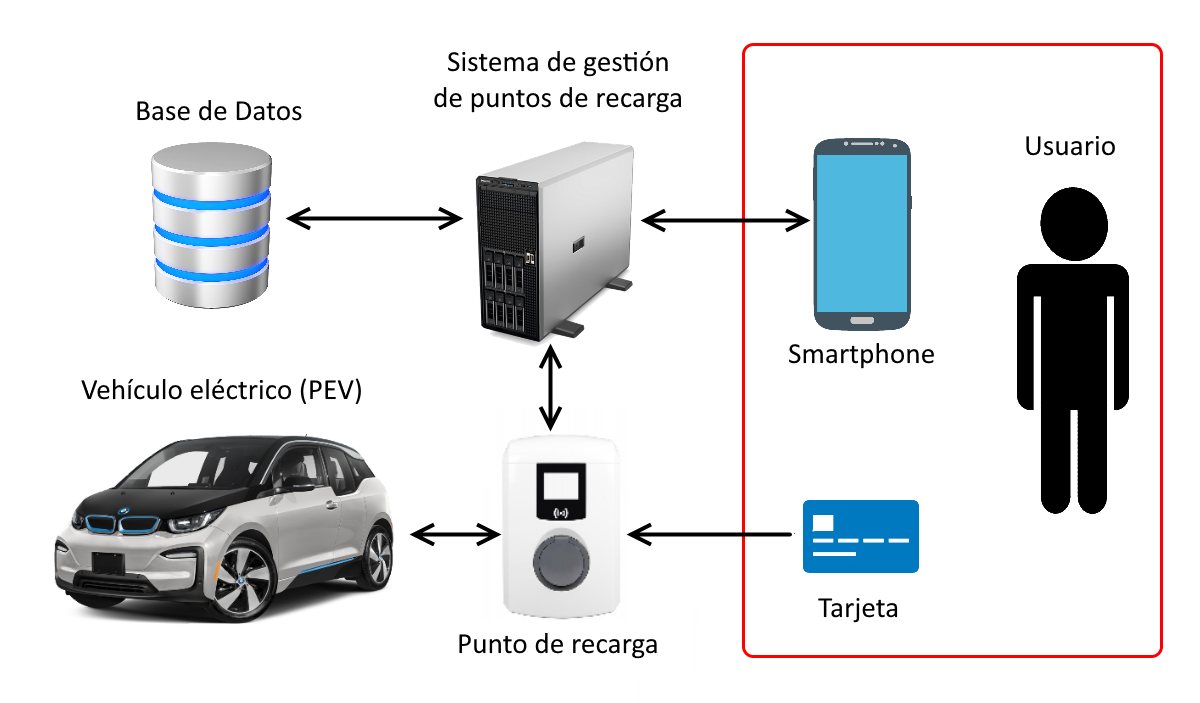
\includegraphics[width=.75\textwidth]{figuras/esquema.png}
  \caption[Arquitectura del sistema propuesto]{Arquitectura del sistema propuesto\\
  }
  \label{fig:arquitectura}
\end{figure}

\begin{enumerate}

\item \textit{Vehículo eléctrico}: El EV crea una comunicación con la estación de carga a través de la línea eléctrica, basándose en el estándar ISO/IEC 15118. En ella, intercambian información sobre la potencia máxima permitida, la capacidad de la batería del vehículo...

\item \textit{Usuario}: El conductor inicia el proceso de recarga a través de una interfaz en el punto de recarga, el uso de algún tipo de tarjeta de fidelización, la utilización de un smartphone o tablet, incluso a distancia desde una interfaz web (también utilizable en un smartphone o tablet) o en algunos casos con un protocolo inalámbrico de amplio rango (por ejemplo, conexión 4G/5G) ya existente en el EV. Además, en algunos casos el conductor puede definir los parámetros de la recarga directamente con el EVSE y monitorear la recarga real. En el caso que se trata, se utilizarán tan solo smartphone (con interfaz web) o con el paso de una tarjeta.

\item \textit{Punto de recarga}: Permite la interoperabilidad con todo tipo de EV, proporciona al usuario distinta información sobre el estado actual del mismo, de la recarga que está realizando o acaba de realizar..., e intercambia información con la base de datos a través del sistema de gestión de puntos de recarga.

\item \textit{Base de datos}: La base de datos almacena datos de los puntos de recargas disponibles en el sistema o en otros sistemas con los que haya algún tipo de acuerdo, de los usuarios autorizados para usar los puntos de recarga, de todas las reservas en estos mismos y la información de facturación... La estructura de la base de datos se tratará más adelante.

\item \textit{CSMS}: Coordina todas las operaciones. Consiste en una aplicación web que maneja las solicitudes tanto del punto de recarga como de la aplicación del usuario del EV e intercambia datos con la base de datos.  El servicio de atención al cliente de la estación central es responsable de proporcionar y recibir información de la aplicación del usuario. En particular, la aplicación envía solicitudes HTTP POST al servidor web, que contiene los datos enviados por parte de los puntos de recarga en formato JSON.

\end{enumerate}


\subsubsection{Protocolo OCPP 1.6}
\label{Protocolo OCPP 1.6}

En este apartado se definirán en profundidad algunos de los conceptos básicos, en especial en torno a algunas características del funcionamiento, el modelo de intercambio de mensajes, la forma de comunicación... del protocolo OCPP 1.6.


\subsubsubsection{Ejemplos de funcionamiento}
\label{Ejemplos de funcionamiento}

Hay dos posibilidades de comunicación entre el punto de recarga y el CSMS en este protocolo. En el primero, es el punto de recarga el que inicia el proceso de comunicación y en la segunda es el CSMS el que lo hace. Dos ejemplos de esto son los siguientes:

\begin{enumerate}

\item En el primero, un punto de recarga solicita la autenticación de una tarjeta o de un identificador enviado por el propio CSMS y envía el estado de la transacción de carga.

\item En el segundo caso, es el CSMS inicia la actualización del firmware de un punto de recarga.

\end{enumerate}

El proceso para el inicio y la detención de una recarga se puede ver en el siguiente diagrama:

\begin{figure}[H] 
\centering
  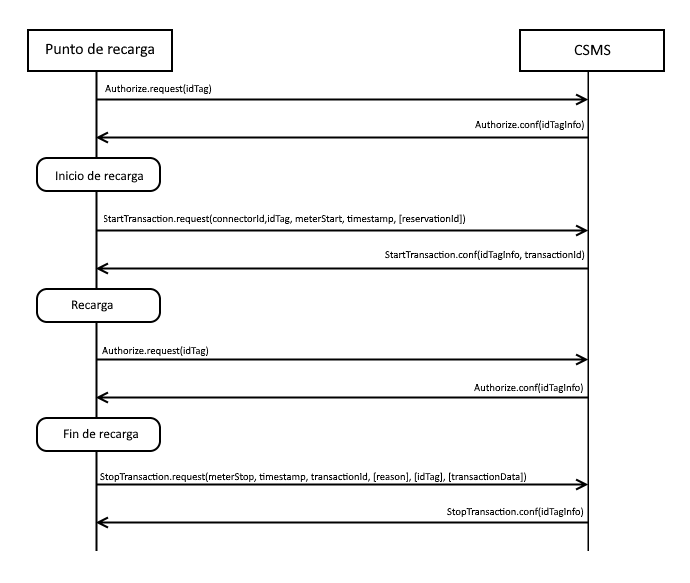
\includegraphics[width=0.9\textwidth]{figuras/diagramainiciofincarga.png}
  \caption[Diagrama de secuencia de una recarga]{Diagrama de secuencia de una recarga\\
  }
  \label{fig:diagramarecarga}
\end{figure}

Cuando un punto de recarga va a cargar a un EV, primero debe autenticar al usuario antes de que se pueda iniciar la carga. Si este está autorizado, el punto de recarga inicia la carga e informa al CSMS que ha iniciado la carga.

Cuando un usuario desea finalizar la recarga y desenchufar el EV del punto de recarga, este debe verificar que es el usuario que inició la carga o que es un usuario distinto pero con permiso para finalizar la recarga. Una vez autorizado, el punto de Recarga informa al CSMS de que se ha finalizado la recarga.

El proceso de actualización de firmware es como el visto a continuación:

\begin{figure}[H] 
\centering
  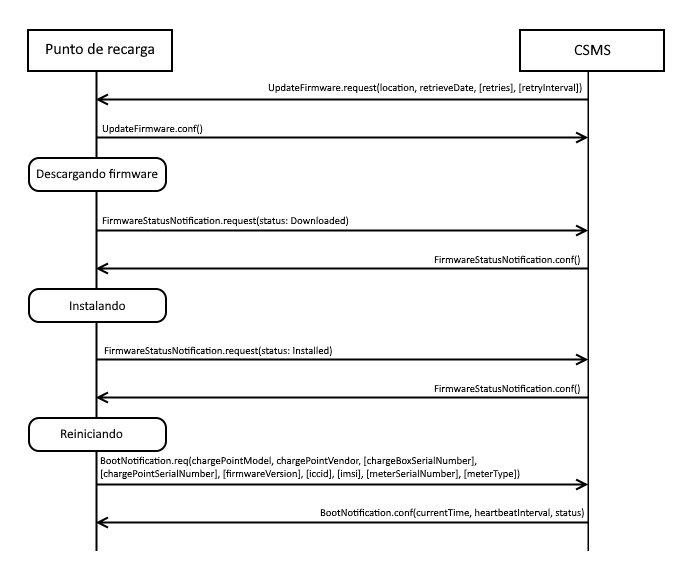
\includegraphics[width=0.9\textwidth]{figuras/diagramaactualizacionfirmware.png}
  \caption[Diagrama de actualización de firmware]{Diagrama de actualización de firmware\\
  }
  \label{fig:diagramaactualizacionfirmware}
\end{figure}

Cuando un punto de recarga necesita una actualización de firmware, el CSMS informa al punto de recarga de la hora en la que este puede comenzar a descargar el nuevo firmware. El punto de recarga debe notificar al CSMS cada paso realizado a medida que se va descargando e instalando el nuevo firmware.

\subsubsubsection{Modos de autorización local y funcionamiento sin conexión}
\label{Modos de autorización local y funcionamiento sin conexión}

En caso de no disponibilidad de las comunicaciones a través de internet o una caída del CSMS, el punto de recarga está diseñado para poder funcionar de forma autónoma. En este caso, se considera al punto de recarga \textit{desconectado} y se marca como tal si funciona el CSMS.

Para mejorar la experiencia de los usuarios, se puede configurar un punto de recarga para admitir la autorización local de identificadores a través una caché de autorización y/o una lista de autorizaciones locales (\textit{whitelist}). Otra opción es el permitir recargar a todo el mundo en caso de que no haya conexión entre punto de recarga y CSMS. 

Esto permite la autorización de un usuario cuando el punto de recarga está desconectado y mejora el tiempo de respuesta de autorización cuando la comunicación entre el punto de recarga y el CSMS es lenta.

Por otro lado, un punto de recarga puede configurarse para admitir la autorización (automática) de cualquier identificador cuando el estado del mismo es de desconectado, para evitar la denegación de servicio y posterior cobro a usuarios de buena fe que no pueden ser autorizados explícitamente por las entradas de la lista de autorización local/caché de autorización. En este caso se desactivará esta autorización automática por motivos de seguridad.


\subsubsubsection{Numeración de conectores}
\label{Numeración de conectores}

Para que el CSMS pueda comunicarse con todos los conectores de un punto de recarga, los ConnectorIds deben estar siempre numerados de la siguiente manera:

\begin{enumerate}

\item El identificador (ConnectorId) del primer conector debe ser 1.
\item Los conectores adicionales deben numerarse de forma secuencial, sin omitir números.
\item Los ConnectorIds nunca deben ser superiores al número total de conectores de un punto de recarga. Si hay tres conectores el número máximo es 3.
item Para operaciones iniciadas por el CSMS o por el punto, se reserva el número 0 de ConnectorId para enviar información general al punto de recarga.
\item Para las operaciones iniciadas por el punto de recarga (informativas), el número 0 de ConnectorId está reservado para el controlador principal del punto de recarga.

\end{enumerate}


\subsubsubsection{Identificadores}
\label{Identificadores}

Los datos adquiridos a través del hardware del lector local de tarjetas suelen ser un valor UID (4 o 7 bytes) de una tarjeta RFID física, representado como 8 o 14 caracteres de dígitos hexadecimales. 

Sin embargo, estos identificadores cuando son enviados a los puntos de recarga por los CSMS para las sesiones de carga iniciadas de forma remota pueden ser códigos de autorización de transacciones virtuales (de un solo uso) o tokens RFID virtuales que utilizan deliberadamente un formato de UID no estándar para evitar posibles conflictos con los valores de UID reales que se utilizan al iniciar la recarga con un paso de tarjeta.

También, en el caso que se verá después de identificadores superiores o de grupo, se puede utilizar otro identificador superior con otro formato cuando hay una cuenta central en la que unos usuarios tienen permiso para detener las recargas de otros usuarios.

Mientras cumpla un formato de \textit{CiString20Type} (cadena de texto de tamaño máximo 20 caracteres) se puede enviar cualquier cosa siempre que se trate de un identificador significativo (que identifique al usuario que inicia o finaliza carga).

Esta parte de la autorización es la que puede estar más comprometida y es en la que se tratará de fortalecer su seguridad a lo largo de este trabajo. Además, se recomienda la representación de estos identificadores en hexadecimal, como ya se mencionó antes.


\subsubsubsection{Identificadores superiores}
\label{Identificadores superiores}

Un CSMS tiene la capacidad de tratar un conjunto de identificadores como un grupo, lo que permite que cualquier identificador de ese grupo inicie una transacción y que el mismo token u otro token del mismo grupo pueda detenerla. Esto es compatible con los casos de uso comunes de familias o empresas con múltiples conductores para una flota de vehículos compartidos que usan en una sola cuenta de contrato de recarga.

Se agrupan con fines de autorización especificando un identificador de grupo superior. Se considera que dos identificadores están en el mismo grupo si disponen de una etiqueta superior que coincida en ambos.

Se trata del mismo caso que un identificador único de un usuario por lo que, al fortalecer la seguridad de este, la protección frente a posibles robos del identificador aplica también en este caso.



\subsubsubsection{Operaciones iniciadas por el punto de recarga}
\label{Operaciones iniciadas por el punto de recarga}

En este apartado se tratarán los modos de comunicación entre punto de recarga y CSMS más relevantes.

\paragraph{Authorize (autorizar)}
\label{Authorize (Autorizar)}


\begin{figure}[H] 
\centering
  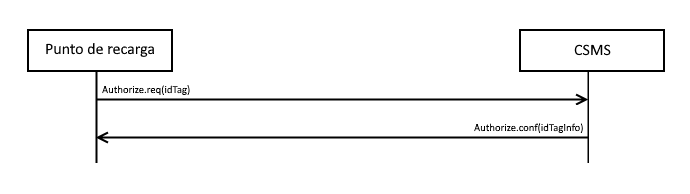
\includegraphics[width=0.9\textwidth]{figuras/diagramaauthorize.png}
  \caption[Diagrama de \textit{Authorize}]{Diagrama de Authorize\\
  }
  \label{fig:diagramaauthorize}
\end{figure}


Antes de que el propietario de un vehículo eléctrico sea capaz de iniciar o detener la carga, el punto de recarga tiene que autorizar la operación. Este solo debería suministrar energía previa autorización. Al detener una transacción, el punto de recarga sólo debería enviar un paquete de autorización cuando el identificador utilizado para detener la transacción es diferente del que inició la transacción.

Un punto de recarga podría autorizar al identificador localmente sin involucrar al CSMS, como se describe en \textit{Modos de autorización local y funcionamiento sin conexión} (\ref{Modos de autorización local y funcionamiento sin conexión}). Si una etiqueta de identificación presentada por el usuario no está en la lista de autorización local o en la memoria caché de autorización el punto de recarga debería enviar una solicitud de autorización al CSMS para solicitar autorización. Si, en caso contrario, está presente en la lista de autorización local o en la memoria caché de autorización, el punto de recarga simplemente podría enviar una solicitud de autorización al CSMS. Si el punto de recarga dispone de una caché de autorización, al recibir una confirmación de autorización, el punto de recarga debe actualizar la entrada de caché dependiendo de si esta tiene permiso o no. En el caso que se trata esta configuración está desactivada.

Al recibir una solicitud de autorización, el CSMS debería responder con una confirmación de autorización. Esta última debe indicar si el CSMS acepta o no la etiqueta de identificación. Si el CSMS acepta esta etiqueta, la confirmación podría incluir una etiqueta de identificación superior y debe incluir un valor de estado de autorización que indique la aceptación o el motivo del rechazo.


\paragraph{BootNotificacion (notificación de arranque)}
\label{BootNotificacion (notificación de arranque)}


\begin{figure}[H] 
\centering
  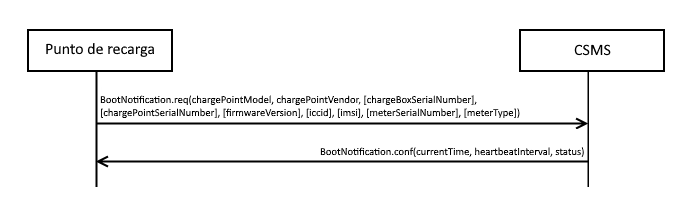
\includegraphics[width=0.9\textwidth]{figuras/diagramabootnotification.png}
  \caption[Diagrama de \textit{BootNotification}]{Diagrama de BootNotification\\
  }
  \label{fig:diagramabootnotification}
\end{figure}


Después de la puesta en marcha un punto de recarga debe enviar una solicitud al CSMS con información sobre su configuración (marca, proveedor, etc.). El CSMS debería responder para indicar si lo acepta en el sistema o no.

El punto de recarga debería enviar una solicitud \textit{BootNotification} cada vez que arranca o reinicia. Entre el encendido/reinicio físico y la finalización exitosa de una \textit{BootNotification}, donde el CSMS devuelve o aceptado o pendiente, el punto de recarga no enviará ninguna solicitud distinta al CSMS. Esto incluye los mensajes antiguos todavía almacenados en la caché del punto de recarga.

Cuando el CSMS responde al \textit{BootNotification} con el estado aceptado, el punto de recarga ajustará el intervalo de Heartbeat (que consisten en avisos periódicos al CSMS de que sigue en funcionamiento y con conexión) de acuerdo con el intervalo que recibe en la confirmación y se recomienda sincronizar su reloj interno con la hora actual del CSMS suministrado. Si el CSMS responde a la solicitud \textit{BootNotification} algo que no sea del valor aceptado, el valor del campo de intervalo indica el tiempo de espera mínimo antes de enviar una próxima solicitud \textit{BootNotification}. Si ese valor de intervalo es cero, el punto de recarga lo elige por su cuenta, para evitar inundar el CSMS con estas solicitudes. Un punto de recarga debe enviar una solicitud \textit{BootNotification} antes de que se supere este tiempo a menos que el CSMS le solicite hacerlo con un mediante una solicitud llamada \textit{TriggerMessage}.

Si el CSMS devuelve el estado rechazado, el punto de recarga no enviará ningún mensaje OCPP al CSMS hasta que haya expirado el mencionado intervalo de reintento. Durante este, es posible que ya no se pueda acceder al punto de recarga desde el CSMS. Este podría cerrar su canal de comunicación o apagar el hardware de comunicación, por ejemplo, para liberar recursos del sistema. Si el estado es rechazado, el punto de recarga no debe responder a ningún mensaje iniciado por el CSMS ni este último debe iniciar ninguna comunicación.

El CSMS podría devolver también un estado pendiente de registro para indicar que se busca recuperar o configurar algún parámetro en el punto de recarga antes de que el CSMS acepte el punto de recarga. Si este devuelve el estado pendiente de registro, el canal de comunicación no debería ser cerrado ni por el punto de recarga ni por el CSMS. El punto de recarga debería responder a estos mensajes y no debería enviar mensajes de solicitud al CSMS a menos que, como se dice anteriormente, este le haya dado instrucciones para hacerlo con una solicitud \textit{TriggerMessage}.

En este estado pendiente de registro, el CSMS no puede iniciar ni una solicitud \textit{RemoteStartTransaction} ni una \textit{RemoteStopTransaction}. Sí debería aceptar transacciones autorizadas mediante caché, aunque estas puedan no entregarse al sistema central. Igualmente, en el caso que se estudia en este trabajo no va a aplicar.

\paragraph{Heartbeat (latido)}
\label{Heartbeat (latido)}


\begin{figure}[H] 
\centering
  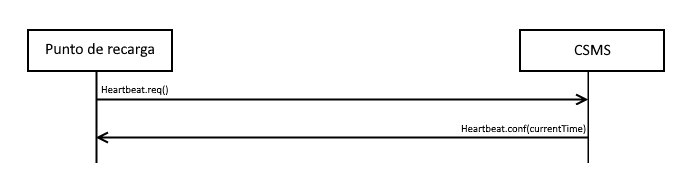
\includegraphics[width=0.9\textwidth]{figuras/diagramaheartbeat.png}
  \caption[Diagrama de \textit{Heartbeat}]{Diagrama de Heartbeat\\
  }
  \label{fig:diagramaheartbeat}
\end{figure}


Para que el CSMS sepa que un punto de recarga se mantiene activo y conectado, un punto de recarga deberá enviar una solicitud \textit{Heartbeat} después de un intervalo de tiempo configurable.

Al recibir una solicitud \textit{Heartbeat}, el CSMS debería responder con una confirmación \textit{Heartbeat}. La confirmación contendrá la hora actual del CSMS, la cual se recomienda utilizar por parte del punto de recarga para sincronizar su reloj interno.

El punto de recarga podría omitir el envío de una solicitud \textit{Heartbeat} cuando se ha enviado otra solicitud al CSMS dentro del intervalo de \textit{Heartbeat} configurado. Esto implica que un CSMS debería asumir la disponibilidad de un punto de recarga siempre que haya recibido una solicitud, de la misma manera que lo habría hecho cuando recibió una solicitud \textit{Heartbeat}.

Con JSON sobre WebSocket el envío de este tipo de paquetes no es obligatorio. Sin embargo, por sincronización horaria, se recomienda enviar al menos uno cada día.


\paragraph{MeterValues (valores del medidor)}
\label{MeterValues (valores del medidor)}


\begin{figure}[H] 
\centering
  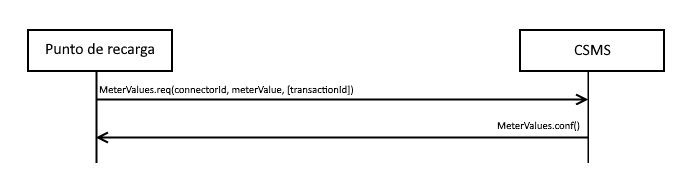
\includegraphics[width=0.9\textwidth]{figuras/diagramametervalues.png}
  \caption[Diagrama de \textit{MeterValues}]{Diagrama de MeterValues\\
  }
  \label{fig:diagramametervalues}
\end{figure}


Un punto de recarga debe muestrear el medidor de energía u otro tipo de hardware sensor o transductor para proporcionar algún tipo de información adicional sobre los valores de este. Depende del punto de recarga la decisión de cuándo enviará los valores del medidor. Esto se puede configurar usando una solicitud llamada \textit{ChangeConfiguration} para configurar los intervalos de adquisición de datos y especificar los datos que se adquirirán y reportarán.

El punto de recarga debe enviar una solicitud \textit{MeterValues} para descargar los valores de contadores. Debe contener el id del conector del que se tomaron las muestras, el id de la transacción a la que se relacionan, si corresponde, y los elementos de valores de \textit{MeterValues}.

En primer lugar, si el \textit{ConnectorId} es 0, el mensaje se asocia a todo el punto de recarga. Si el \textit{ConnectorId} es 0 y la magnitud está relacionada con la energía, esta muestra debe tomarse del medidor de energía principal.

Por otro lado, si no hay una transacción en curso o si los valores se toman del medidor principal se puede omitir el \textit{TransactionId}. 

Finalmente, los valores del \textit{MeterValues}, cada uno de los cuales representa un conjunto de uno o más valores de datos recogidos en un momento determinado.

Cada elemento \textit{MeterValues} contiene una marca de tiempo y un conjunto de uno o más elemento de valor de muestreo, todos capturados en el mismo momento. Cada elemento de valor muestreado contiene un único dato de valor. La naturaleza de cada valor muestreado está determinada por los opcionales \textit{magnitud}, \textit{contexto}, \textit{ubicación}, \textit{unidad}, \textit{fase}, y el \textit{formato de campos}.

El campo opcional \textit{magnitud} especifica el tipo de valor que se mide/informa.

El campo opcional \textit{contexto} especifica el motivo/evento que desencadena la lectura del medidor.

El campo opcional \textit{ubicación} especifica dónde se toma la medición (p. ej., entrada, salida).

El campo opcional fase especifica a qué fase o fases de la instalación eléctrica se aplica el valor. El punto de recarga debería informar de todos los valores dependientes del número de fase desde el punto de vista del medidor de energía (o la conexión a la red cuando esté ausente). Igualmente, este campo no es aplicable a todos los tipos de medidas. Por otro lado, hay están dos valores disponibles que estrictamente hablando no se refieren a valores medidos en ningún momento puntual. Estos se refieren a la cantidad máxima de corriente/potencia que se ofrece al EV y están destinados para su uso en aplicaciones de carga inteligente.

Para la información de rotación de fase de un conector individual, el CSMS puede consultar la configuración del mismo en el punto de recarga con la opción \textit{ConnectorPhaseRotation} mediante un paquete llamado \textit{GetConfiguration}. El punto de recarga debe informar de la rotación de fases con respecto a la conexión a la red. Los valores configurables por conector son \textit{NotApplicable}, \textit{Unknown}, \textit{RST}, \textit{RTS}, \textit{SRT}, \textit{STR}, \textit{TRS} y \textit{TSR}. 

El campo experimental \textit{formato} especifica si los datos se representan en la forma normal (predeterminada) como un valor numérico simple (\textit{crudo}), o como \textit{datos firmados}, un bloque de datos binarios con firma digital opaca, representado como datos hexadecimales. Este campo experimental podría quedar obsoleto y más adelante eliminado en versiones posteriores cuando se proporcione una alternativa de solución más madura.

Para mantener la compatibilidad con versiones anteriores, los valores predeterminados de todos los campos opcionales en un elemento de valor muestreado son tales que un valor sin ningún campo adicional se interpretará como una lectura de registro de energía de importación activa en unidades de Wh (watios hora).

Es probable que el CSMS haga alguna comprobación sobre los datos obtenidos de una solicitud \textit{MeterValues}. El resultado de tales comprobaciones no debe generar que el CSMS no responda con una confirmación \textit{MeterValues}. No responder correctamente hará que el punto de recarga vuelva a intentar el mismo mensaje.



\paragraph{StartTransaction (iniciar transacción)}
\label{StartTransaction (iniciar transacción)}


\begin{figure}[H] 
\centering
  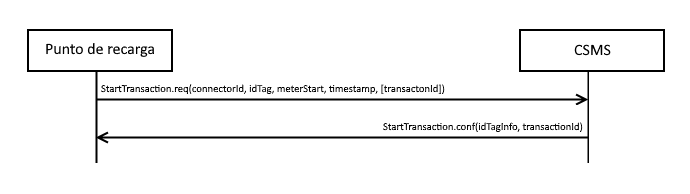
\includegraphics[width=0.9\textwidth]{figuras/diagramastarttransaction.png}
  \caption[Diagrama de \textit{StartTransaction}]{Diagrama de StartTransaction\\
  }
  \label{fig:diagramastarttransaction}
\end{figure}


El punto de recarga debe enviar una solicitud StartTransaction al CSMS para informar sobre el inicio de una transacción. Si esta transacción se corresponde con una reserva, la solicitud \textit{StartTransaction} tendrá que contener el identificador de la reserva.

Al recibir una solicitud \textit{StartTransaction}, el CSMS deberá de responder con una confirmación \textit{StartTransaction}. Este mensaje de confirmación debe incluir una identificación de transacción y un valor de estado de autorización.

El CSMS debería verificar la validez del identificador en la solicitud \textit{StartTransaction} recibida, porque el identificador podría haber sido autorizado localmente por la caché de autorización existente en el punto de recarga utilizando información desactualizada. El identificado, por ejemplo, puede haber sido bloqueado en el CSMS en el intervalo en la última conexión del punto de recarga con él y en la llegada del \textit{StartTransaction}. Tras recibir un \textit{StartTransaction} debe actualizar la entrada de caché si es que ese identificador no está en la misma. En cualquier caso, en este trabajo no va a aplicarse esta configuración.

Es probable que el CSMS haga alguna comprobación sobre los datos obtenidos de una solicitud \textit{StartTransaction}. El resultado de tales comprobaciones no debe generar que el CSMS no responda con una confirmación \textit{StartTransaction}. No responder correctamente hará que el punto de recarga vuelva a intentar el mismo mensaje.


\paragraph{StatusNotification (notificación de estado)}
\label{StatusNotification (notificación de estado)}


\begin{figure}[H] 
\centering
  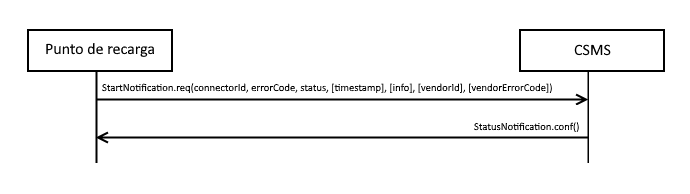
\includegraphics[width=0.9\textwidth]{figuras/diagramastatusnotification.png}
  \caption[Diagrama de \textit{StatusNotification}]{Diagrama de StatusNotification\\
  }
  \label{fig:diagramastatusnotification}
\end{figure}



Un punto de recarga envía una notificación al CSMS para informarle sobre un cambio de estado o un error dentro del punto de recarga. La siguiente tabla muestra todos los posibles estados con los cambios de un estado anterior (columna izquierda) a un estado nuevo (fila superior) en el que un punto de recarga puede enviar una solicitud \textit{StatusNotification} al CSMS.

Los posibles estados del punto de recarga y su denominación en la tabla de estados son:


\begin{enumerate}

\item Available (A, 1): disponible.
\item Preparing (B, 2): preparando.
\item Charging (C, 3): cargando.
\item Suspended EV (D, 4): EV suspendido.
\item Suspended EVSE (E, 5): EVSE suspendido.
\item Finishing (F, 6): Finalizando.
\item Reserved (G, 7): Reservado.
\item Unavailable (H, 8): No disponible.
\item Faulted (I, 9): Fallado.

\end{enumerate}


% Please add the following required packages to your document preamble:
% \usepackage{booktabs}
\begin{longtable}{|p{0.05\textwidth}|p{0.05\textwidth}|p{0.05\textwidth}|p{0.05\textwidth}|p{0.05\textwidth}|p{0.05\textwidth}|p{0.05\textwidth}|p{0.05\textwidth}|p{0.05\textwidth}|p{0.05\textwidth}|p{0.05\textwidth}|}
\caption{Estados del punto de recarga y su tabla de flujo}
\label{tablaestadospuntoderecarga}
\endfirsthead
\endhead
\hline
 & \hspace{0pt}1 & \hspace{0pt}2 & \hspace{0pt}3 & \hspace{0pt}4 & \hspace{0pt}5 & \hspace{0pt}6 &  & \hspace{0pt}7 & \hspace{0pt}8 & \hspace{0pt}9 \\ \hline
 A & - & A2 & A3 & A4 & A5 & - &  & A7 & A8 & A9 \\
 B & B1 & - & B3 & B4 & B5 & - &  & - & - & B9 \\
 C & C1 & - & - &  C4 & C5 & C6 &  & - & C8 & C9 \\ 
 D & D1 & - & D3 & - & D5 & D6 &  & - & D8 & D9 \\ 
 E & E1 & - & E3 & E4 & - & E6 &  & - & E8 & E9 \\ 
 F & F1 & F2 & - & - & - & - &  & - & F8 & F9 \\ 
  &  &  &  &  &  &  &  &  &  &  \\ 
 G & G1 & G2 & - & - & - & - &  & - & G8 & G9 \\ 
 H & H1 & H2 & H3 & H4 & H5 & - &  & - & - & H9 \\ 
 I & I1 & I2 & I3 & I4 & I5 & I6 &  & I7 & I8 & - \\ \hline
\end{longtable}

La siguiente tabla describe los eventos que pueden llevar a un cambio de estado:

\begin{longtable}{|p{1cm}|p{14cm}|}
\caption{Eventos que pueden llevar a cambios de estado}
\label{Eventos que pueden llevar a cambios de estado}
\endfirsthead
\endhead
\hline
- & No es posible \\ 
 & \\
A2 & Se inicia el uso (por ejemplo, se enchufa el vehículo, se pasa una etiqueta de identificación, se recibe una solicitud de RemoteStartTransaction...) \\ 
A3 & Podría ser posible en un punto de recarga sin la obligación de autorizarse activa \\ 
A4 & Similar al A3 pero el EV no comienza a cargar \\ 
A5 & Similar al A3 pero el EVSE no comienza a cargar \\ 
A7 & Se recibe un mensaje \textit{ReserveNow} (reservar ahora) \\ 
A8 & Se recibe un mensaje \textit{ChangeAvailability} (cambio de disponibilidad) que marca el conector como \textit{Unavailable} \\
A9 & Se detecta un fallo que impide posteriores operaciones de carga \\ 
 & \\
B1 & Se finaliza el uso previsto (por ejemplo, se desenchufa el vehículo, se pasa por segunda vez una etiqueta de identificación, se agota el tiempo de espera hasta una acción del usuario...) \\
B3 & Se cumplen todos los requisitos previos para iniciar la carga y comienza el proceso\\
B4 & Se cumplen todos los requisitos previos para la carga, pero el EV no comienza a cargar \\
B5 & Se cumplen todos los requisitos previos para la carga, pero el EVSE no comienza a cargar \\
B9 & Se detecta un fallo que impide posteriores operaciones de carga \\
 & \\
C1 & La sesión de carga finaliza sin haberse requerido ninguna acción por parte del usuario (por ejemplo, se quitó la manguera en el lado del EV)\\
C4 & La carga se detiene cuando lo solicita el EV\\
C5 & La carga se detiene cuando lo solicita el EVSE (por ejemplo, restricción de carga inteligente, la transacción es invalidada por una solicitud AuthorizationStatus en una confirmación StartTransaction)\\
C6 & La sesión de carga es detenida por el usuario o un RemoteStopTransaction y se requiere una acción adicional del usuario consistente en quitar el cable\\
C8 & La sesión de carga finaliza, no se requiere ninguna acción del usuario y el conector está programado para ponerse en el estado \textit{Unavailable}\\
C9 & Se detecta un fallo que impide posteriores operaciones de carga \\
 & \\
D1 & La sesión de carga finaliza sin haberse requerido ninguna acción por parte del usuario (por ejemplo, se quitó la manguera en el lado del EV)\\
D3 & La carga se reanuda a petición del EV\\
D5 & EVSE suspende la carga\\
D6 & La sesión de carga se detiene y se requiere más acción del usuario (quitar el cable)\\
D8 & La sesión de carga finaliza, no se requiere ninguna acción del usuario y el conector está programado para ponerse en el estado \textit{Unavailable}\\
D9 & Se detecta un fallo que impide posteriores operaciones de carga \\
 & \\
E1 & La sesión de carga finaliza sin haberse requerido ninguna acción por parte del usuario (por ejemplo, se quitó la manguera en el lado del EV)\\
E3 & La carga se reanuda porque se levanta la petición EVSE\\
E4 & Se levanta la petición EVSE pero el EV no comienza a cargar\\
E6 & La sesión de carga se detiene y se requiere más acción del usuario (quitar el cable)\\
E8 & La sesión de carga finaliza, no se requiere ninguna acción del usuario y el conector está programado para ponerse en el estado \textit{Unavailable}\\
E9 & Se detecta un fallo que impide posteriores operaciones de carga \\
 & \\
F1 & Completadas todas las acciones del usuario \\
F2 & El usuario reinicia la sesión de carga (por ejemplo, se vuelve a enchufar el vehículo, se vuelve a pasar una etiqueta de identificación...) \\ 
F8 & Se completan todas las acciones del usuario y el conector está programado para ponerse en el estado \textit{Unavailable}\\
F9 & Se detecta un fallo que impide posteriores operaciones de carga \\
 & \\
G1 & La reserva caduca o se recibe un mensaje \textit{CancelReservation} (cancelación de reserva)\\
G2 & Se presenta la identidad de la reserva\\
G8 &  La reserva caduca o se recibe un mensaje \textit{CancelReservation} (cancelación de reserva) y el conector está programado para ponerse en el estado \textit{Unavailable}\\
G9 & Se detecta un fallo que impide posteriores operaciones de carga \\
 & \\
H1 & El conector se configura como \textit{Disponible} después de que llegase un mensaje \textit{ChangeAvailability} (cambiar disponibilidad)\\
H2 & El conector se configura como \textit{Disponible} después de que el usuario haya interactuado con el punto de recarga\\
H3 & El conector se configura como \textit{Disponible} y no se requiere ninguna acción del usuario para comenzar a cargar\\
H4 & Similar a H3 pero el EV no comienza a cargar\\
H5 & Similar a H3 pero el EVSE no comienza a cargar\\
H9 & Se detecta un fallo que impide posteriores operaciones de carga \\
 & \\
I1-I8 & El fallo se resuelve y el estado vuelve al estado previo al fallo \\
\hline
\end{longtable}


Estas tablas solo aplican cuando el \textit{ConnectorId} es mayor que 0. Para el \textit{ConnectorId} 0, que se refiere al general del punto, solo están disponibles los estados \textit{Available}, \textit{Unavailable}, \textit{Faulted}. El estado de \textit{ConnectorId} 0 no tiene conexión directa con el estado de los conectores individuales mayores que 0.

Por otro lado, si tanto el EV como el EVSE suspenden la carga, el estado \textit{SuspendedEVSE} tendrá prioridad sobre el estado SuspendedEV.

Cuando un punto de recarga o un conector cambian su estado a \textit{Unavailable} por una solicitud \textit{ChangeAvailability}, el estado \textit{Unavailable} debería ser persistente en todos los reinicios. El punto de recarga puede utilizar el estado \textit{Unavailable} internamente para otros fines (por ejemplo, mientras se actualiza el firmware)

Ya que el estado \textit{Occupied} se ha subdividido en cinco nuevos estados (\textit{Preparing}, \textit{Charging}, \textit{SuspendedEV}, \textit{SuspendedEVSE} y \textit{Finishing}), se envían más solicitudes StatusNotification. Estas se enviarán desde el punto de recarga al CSMS. Por ejemplo, cuando se inicia una transacción, el estado del conector cambiaría sucesivamente de \textit{Preparing} a \textit{Charging} con un corto \textit{SuspendedEV} y/o \textit{SuspendedEVSE} en el medio, con una duración de en torno a un par de segundos.

Para limitar el número de cambios de estado, el punto de recarga puede omitir el envío de una solicitud \textit{StatusNotification} si estuvo activo menos tiempo del definido en la clave de configuración opcional \textit{MinimumStatusDuration} (duración mínima del estado). De esta forma, un punto de recarga puede optar por no enviar algunas solicitudes \textit{StatusNotification}. Por otro lado, un fabricante de puntos de recarga puede haber implementado una duración de estado mínima (retardo) para ciertas transiciones de estado separadas de la opción \textit{MinimumStatusDuration}. El tiempo establecido en \textit{MinimumStatusDuration} se agregará a este retraso predeterminado. Ajustar \textit{MinimumStatusDuration} a cero no anula la duración de estado mínima predeterminada del fabricante. Establecer un valor alto de este parámetro podría retrasar todas las notificaciones de estado, ya que el punto de recarga solo lo mandaría después de que pasase ese tiempo.

El punto de recarga puede enviar una solicitud \textit{StatusNotification} para informar al CSMS de algunas condiciones que producen un fallo. Cuando el campo estado no está \textit{Faulted} esa condición debe considerarse una advertencia, ya que las operaciones de carga aún son posibles.

El \textit{ChargePointErrorCode} (código de error de punto de carga \textit{EVCommunicationError} solo deberá usarse con el estado \textit{Preparing}, \textit{SuspendedEV}, \textit{SuspendedEVSE} y \textit{Finishing} y se tratará como si fuese una advertencia.

Cuando un punto de recarga está configurado con \textit{StopTransactionOnEVSideDisconnect} (detener la transacción tras desconexión del lado EV) configurado a falso, se está realizando una carga y esta se desconecta del lado del EV, el estado \textit{SuspendedEV} debería enviarse al CSMS mediante una solicitud \textit{StatusNotification}, con el campo \textit{errorCode} establecido en \textit{NoError}. El punto de recarga entonces tiene que añadir información adicional en el campo \textit{info}, notificando al CSMS con el motivo de la suspensión de la recarga, que sería \textit{EV side disconnected} (lado EV desconectado). La transacción actual no se detiene.

Sin embargo, cuando un punto de recarga está configurado con \textit{StopTransactionOnEVSideDisconnect} fijado a verdadero, se
está ejecutando una carga y el EV se desconecta del lado del EV, se debería enviar al CSMS una solicitud \textit{StatusNotification} con el estado \textit{Finishing}, con el campo \textit{errorCode} establecido en \textit{NoError}. El punto de recarga debería añadir información adicional en el campo \textit{info}, notificando al CSMS con el motivo de la suspensión de la recarga, que sería \textit{EV side disconnected} (lado EV desconectado). La transacción actual no se detiene.

Cuando un punto de recarga se conecta a un CSMS después de haber sido desconectado, actualiza al CSMS sobre su estado de acuerdo con las siguientes reglas:

\begin{itemize}
\item El punto de recarga debería enviar una solicitud \textit{StatusNotification} con su estado actual si es que este cambió mientras el punto de recarga estaba desconectado.
\item El punto de recarga puede enviar una solicitud \textit{StatusNotification} para informar de un error que sucedió cuando el punto de recarga estaba desconectado.
\item El punto de recarga no debe enviar una solicitud \textit{StatusNotification} para eventos de cambio de estado históricos que
ocurrieron mientras el punto de recarga estaba fuera de línea y que no informan al CSMS de errores del propio punto de recarga o de su estado actual.
\item Las solicitudes \textit{StatusNotification} deben enviarse en el orden en el que ocurrieron los eventos que se describen en ellos.

\end{itemize}

Al recibir una solicitud \textit{StatusNotification} el CSMS debería responder con una confirmación \textit{StatusNotification}

\paragraph{StopTransaction (detener transacción)}
\label{StopTransaction (detener transacción)}


\begin{figure}[H] 
\centering
  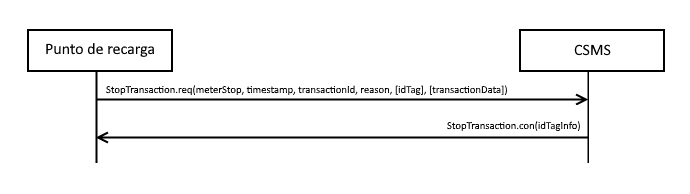
\includegraphics[width=0.9\textwidth]{figuras/diagramastoptransaction.png}
  \caption[Diagrama de \textit{StopTransaction}]{Diagrama de StopTransaction\\
  }
  \label{fig:diagramastoptransaction}
\end{figure}

Cuando se detiene una carga, el punto de recarga debe enviar una solicitud \textit{StopTransaction}, notificando al CSMS que esta se ha detenido.

A una solicitud \textit{StopTransaction} puede contener un opcional \textit{TransactionData} (datos de la transacción) para proporcionar más detalles sobre el uso de transacciones. Este elemento es un contenedor para cualquier número de \textit{MeterValues}, utilizando la misma estructura de datos que los elementos \textit{meterValue} de la solicitud \textit{MeterValues}.

Al recibir una solicitud \textit{StopTransaction}, el CSMS debería responder con una confirmación \textit{StopTransaction}.

El CSMS no puede evitar que una transacción se detenga. Únicamente puede informar al punto de recarga que ha recibido la solicitud \textit{StopTransaction} y puede enviar información sobre la etiqueta de identificación utilizada para detener la transacción. Esta información se utilizará para actualizar la caché de autorización, si se implementa. En este trabajo no se va a implementar.

La etiqueta de identificación en la solicitud puede omitirse cuando el punto de recarga necesita detener la transacción. Por ejemplo, cuando se solicita el reinicio del punto de recarga.

Si una transacción finaliza de forma normal, el elemento \textit{Razón} se puede omitir y debería asumirse como \textit{Local}. Si la transacción no finaliza normalmente, este debe establecerse en un valor correcto. Como parte de la finalización normal de la transacción, el punto de recarga debería desbloquear el cable si es que este no está conectado permanentemente.

El punto de recarga puede detener una transacción en curso cuando se desconecta el cable del vehículo eléctrico. Si esta funcionalidad es compatible, es informada y controlada por la clave de configuración \textit{StopTransactionOnEVSideDisconnect}. Si se establece en falso, la transacción no se debe detener cuando el cable se desconecta del EV. Si se vuelve a conectar el EV, se permitiría nuevamente la transferencia de energía. En este caso, no hay ningún tipo de mecanismo para evitar que otros vehículos eléctricos distintos se carguen y desconecten durante la misma transacción en curso. Con \textit{UnlockConnectorOnEVSideDisconnect} ajustado a falso, el conector debería permanecer bloqueado en el punto de recarga hasta que el usuario detenga la recarga. En caso de que \textit{StopTransactionOnEVSideDisconnect} sea falso, tiene prioridad sobre \textit{UnlockConnectorOnEVSideDisconnect}. En otras palabras, los cables siempre permanecen bloqueados cuando el cable está desconectado en el lado EV al estar fijado \textit{StopTransactionOnEVSideDisconnect} en falso. Configurando \textit{StopTransactionOnEVSideDisconnect} a verdadero, la transacción se debería detener cuando el cable se desconecte del EV. Si se vuelve a conectar el EV, no se permitiría la transferencia de energía hasta que se detenga la transacción y se iniciará una nueva transacción. Si \textit{UnlockConnectorOnEVSideDisconnect} se configura a verdadero, también se desbloqueará el conector del punto de recarga. En este trabajo, \textit{StopTransactionOnEVSideDisconnect} se configurará a verdadero y  \textit{UnlockConnectorOnEVSideDisconnect} a falso. Esto evitará que un usuario no autorizado libere un vehículo conectado al punto de recarga para posteriormente conectar el suyo y cargar sin permiso.

Es probable que el CSMS aplique controles de cordura a los datos contenidos en una solicitud \textit{StopTransaction} recibida. El resultado de tales verificaciones de cordura no puede provocar que el CSMS no responda con una confirmación StopTransaction. No responder con ella solo hará que el punto de recarga vuelva a intentar el mismo mensaje.

Si el punto de recarga ha implementado un caché de autorización, luego de recibir una solicitud \textit{StopTransaction}, el punto de recarga debe actualizar la entrada de caché, si la etiqueta de identificación no está en la lista de autorizaciones locales, con el valor \textit{IdTagInfo} de la confirmación como se describe en la caché de autorización. En este caso no aplica.



\subsubsubsection{Operaciones iniciadas por el CSMS}
\label{Operaciones iniciadas por el CSMS}


\paragraph{ChangeConfiguration (cambiar configuración)}
\label{ChangeConfiguration (cambiar configuración)}


\begin{figure}[H] 
\centering
  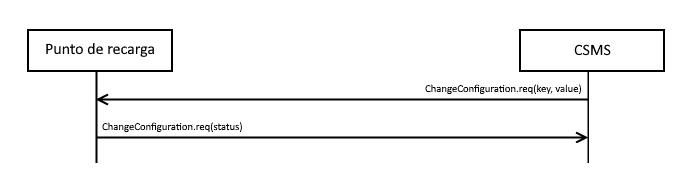
\includegraphics[width=0.9\textwidth]{figuras/diagramachangeconfiguration.png}
  \caption[Diagrama de \textit{ChangeConfiguration}]{Diagrama de ChangeConfiguration\\
  }
  \label{fig:diagramachangeconfiguration}
\end{figure}

El CSMS puede hacer una solicitud a un punto de recarga para cambiar los parámetros de configuración. Para lograr esto, el CSMS debe enviar una solicitud llamada \textit{ChangeConfiguration}. Esta solicitud contiene un par \textit{key-value}, donde \textit{key} (clave) es el nombre de la configuración que se va a cambiar y \textit{value} (valor) contiene el nuevo valor para la configuración.

Al recibir una solicitud \textit{ChangeConfiguration} el punto de recarga deberá enviar una confirmación \textit{ChangeConfiguration} indicando si fue capaz de ejecutar el cambio. El contenido de \textit{key} y \textit{valor} no está predefinido. Si \textit{key} no corresponde a un ajuste de configuración compatible con el punto de recarga, este responderá con un estado \textit{NotSupported} (no compatible). Si por el contrario el cambio se ejecutó de manera exitosa se responderá con un estado \textit{Accepted} (aceptado). Si el cambio se ejecutó correctamente, pero es necesario reiniciar el punto de recarga para aplicarlo, la confirmación contendrá el estado \textit{RebootRequired} (reinicio requerido). En caso de no establecer la nueva configuración, el punto de recarga deberá responder con el estado \textit{Rejected} (rechazado).


\paragraph{ClearCache (limpiar caché)}
\label{ClearCache (limpiar caché)}


\begin{figure}[H] 
\centering
  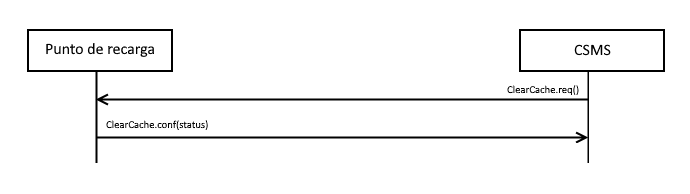
\includegraphics[width=0.9\textwidth]{figuras/diagramaclearcache.png}
  \caption[Diagrama de \textit{ClearCache}]{Diagrama de ClearCache\\
  }
  \label{fig:diagramaclearcache}
\end{figure}

El CSMS puede solicitar a un punto de recarga que borre su caché de autorización. El CSMS tiene que enviar una solicitud \textit{ClearCache} para borrar la memoria de la caché de autorización del punto de recarga. El punto de recarga tendrá que responder con una confirmación \textit{ClearCache}, la cual debe indicar si el punto de recarga pudo borrar esta caché de autorización. En este trabajo no será necesario al no estar configurada.


\paragraph{GetConfiguration (obtener configuración)}
\label{GetConfiguration (obtener configuración)}



\begin{figure}[H] 
\centering
  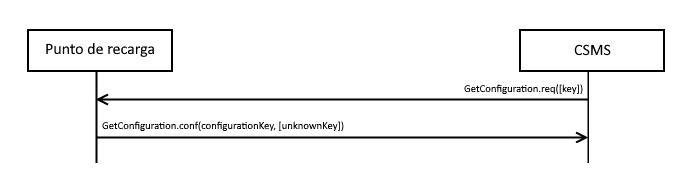
\includegraphics[width=0.9\textwidth]{figuras/diagramagetconfiguration.png}
  \caption[Diagrama de \textit{GetConfiguration}]{Diagrama de GetConfiguration\\
  }
  \label{fig:diagramagetconfiguration}
\end{figure}


Para recuperar el valor de los ajustes de configuración, el CSMS enviará una solicitud \textit{GetConfiguration} al punto de recarga. Si la lista de claves en la PDU está vacía o falta (es opcional), el punto de recarga debe devolver una lista de todos los ajustes de configuración en la confirmación \textit{GetConfiguration}. De lo contrario, el punto de recarga deberá devolver una lista de claves reconocidas y sus valores correspondientes y estado de solo lectura. Las claves no reconocidas deberían colocarse en la confirmación del punto de recarga como parte del elemento opcional de la lista de claves desconocidas.

El punto de recarga podría limitar el número de claves de configuración solicitadas en una sola solicitud. Este máximo se podría recuperar leyendo la clave de configuración \textit{GetConfigurationMaxKeys}.


\paragraph{RemoteStartTransaction (inicio de recarga remoto)}
\label{RemoteStartTransaction (inicio de recarga remoto)}


\begin{figure}[H] 
\centering
  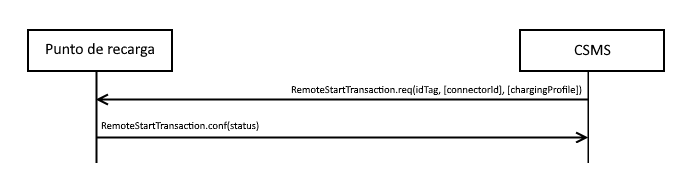
\includegraphics[width=0.9\textwidth]{figuras/diagramaremotestarttransaction.png}
  \caption[Diagrama de \textit{RemoteStartTransaction}]{Diagrama de RemoteStartTransaction\\
  }
  \label{fig:diagramaremotestarttransaction}
\end{figure}



El CSMS puede solicitar un punto de recarga para iniciar una transacción enviando una solicitud \textit{RemoteStartTransaction}. Tras la recepción, el punto de recarga deberá responder con una confirmación \textit{RemoteStartTransaction} y un estado que indica si puede iniciar una transacción o no.

El funcionamiento del mensaje de solicitud \textit{RemoteStartTransaction} depende del valor de la clave de configuración \textit{AuthorizeRemoteTxRequestsclave} de configuración en el punto de recarga.

Si el valor de esta clave \textit{AuthorizeRemoteTxRequests} es verdadero, el punto de recarga debería comportarse como si respondiera a una acción local en el punto de recarga para iniciar una transacción con la etiqueta de identificación proporcionada en el mensaje de solicitud de \textit{RemoteStartTransaction}. Esto significa, por tanto que el punto de recarga primero intentará autorizar la etiqueta de identificación, utilizando o la lista de autorizaciones locales, o la caché de autorización y/o una solicitud \textit{Authorize}. Una transacción solo se iniciará después de que se haya obtenido esta autorización. Por otro lado, si el valor de esta clave es falso, el punto de recarga debe intentar inmediatamente iniciar una transacción para la etiqueta de identificación proporcionada en el mensaje de solicitud de \textit{RemoteStartTransaction}. Tenga en cuenta que una vez iniciada la transacción, el punto de recarga le enviará un \textit{StartTransaction} al CSMS, y el CSMS verificará el estado de autorización de la etiqueta de identificación al procesar esta solicitud de \textit{StartTransaction}.

Estos son los casos más habituales de \textit{RemoteStartTransaction}:
\begin{itemize}
\item Permitir que un operador de CPO ayude a un conductor de EV que tiene problemas para iniciar una transacción.
\item Habilitar aplicaciones móviles para controlar transacciones de cobro a través del CSMS.
\item Habilitar el uso de SMS para controlar transacciones de cobro a través del CSMS.

\end{itemize}

Las solicitudes \textit{RemoteStartTransaction} deben contener un identificador (\textit{idTag}) que el punto de recarga debe utilizar, si puede iniciar una transacción, para enviar una solicitud \textit{StartTransaction} al CSMS. La transacción se inicia de la misma manera que se describe en \textit{StartTransaction}. Las solicitudes \textit{RemoteStartTransaction} pueden contener una identificación de conector si la transacción se va a iniciar en un conector específico. Cuando no se proporciona una identificación de conector, el punto de recarga tiene el control de la selección del mismo. Un punto de recarga podría rechazar un \textit{RemoteStartTransaction} sin una identificación del conector.


\paragraph{RemoteStopTransaction (detención de recarga remoto)}
\label{RemoteStopTransaction (detención de recarga remoto)}


\begin{figure}[H] 
\centering
  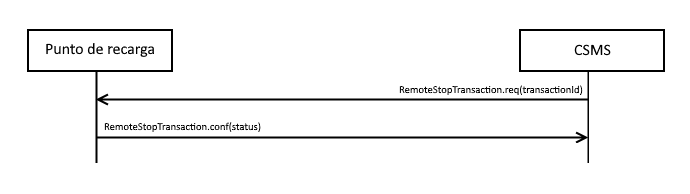
\includegraphics[width=0.9\textwidth]{figuras/diagramaremotestoptransaction.png}
  \caption[Diagrama de \textit{RemoteStopTransaction}]{Diagrama de RemoteStopTransaction\\
  }
  \label{fig:diagramaremotestoptransaction}
\end{figure}


El CSMS puede solicitar a un punto de recarga que detenga una transacción enviando una solicitud \textit{RemoteStopTransaction} al punto de recarga con el identificador de la transacción. El punto de recarga debería responder con una confirmación \textit{RemoteStopTransaction} para indicar si está capacitado para detener la transacción.

Esta solicitud remota para detener una transacción es igual a una acción local para detener una transacción. Por tanto, si la transacción es detenida, el punto de recarga enviará una solicitud \textit{StopTransaction} y, en su caso, desbloquear el conector.

Estos son los casos más habituales de \textit{RemoteStopTransaction}:
\begin{itemize}
\item Permitir que un operador de CPO ayude a un conductor de EV que tiene problemas para detener una transacción.
\item Habilitar aplicaciones móviles para controlar transacciones de cobro a través del CSMS.

\end{itemize}


\paragraph{Reset (reiniciar)}
\label{Reset (reiniciar)}


\begin{figure}[H] 
\centering
  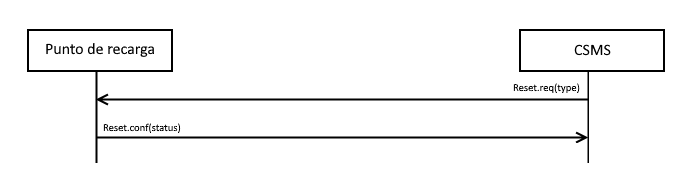
\includegraphics[width=0.9\textwidth]{figuras/diagramareset.png}
  \caption[Diagrama de \textit{Reset}]{Diagrama de Reset\\
  }
  \label{fig:diagramareset}
\end{figure}


El CSMS debería enviar una solicitud \textit{Reset} para solicitar que un punto de recarga se reinicie. El CSMS puede solicitar un restablecimiento completo o parcial. Al recibir una solicitud \textit{Reset}, el punto de recarga debería responder con una confirmación \textit{Reset}. La confirmación debe incluir si el punto de recarga acepta y, por tanto, intenta el reinicio.

Al recibir un restablecimiento parcial, el punto de recarga debería volver a un estado en el que se comporte como si acabara de arrancar. Si alguna transacción está en progreso, debería terminarse normalmente, antes del reinicio, como en un \textit{StopTransaction}.

Al recibir un restablecimiento completo, el punto de recarga debería intentar finalizar cualquier transacción en curso normalmente como en \textit{StopTransaction} y luego realizar un reinicio.


\paragraph{UnlockConnector (desbloqueo de conector)}
\label{UnlockConnector (desbloqueo de conector)}


\begin{figure}[H] 
\centering
  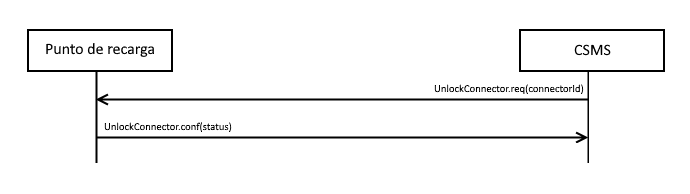
\includegraphics[width=0.9\textwidth]{figuras/diagramaunlockconnector.png}
  \caption[Diagrama de \textit{UnlockConnector}]{Diagrama de UnlockConnector\\
  }
  \label{fig:diagramaunlockconnector}
\end{figure}


El CSMS puede solicitar a un punto de recarga desbloquear un conector. Para ello, el punto de recarga debería enviar una solicitud \textit{UnlockConnector}

El objetivo de este mensaje es el de ayudar a los conductores de EV que tienen problemas para desconectar el cable del punto de carga en caso de algún tipo de mal  no esperado funcionamiento de la retención del cable del conector. Cuando un conductor de un EV llama al \textit{help-desk} de CPO, un operador podría activar manualmente el envío de una solicitud \textit{UnlockConnector} al punto de recarga, obligando a un nuevo intento de desbloqueo del conector. Si todo va según lo previsto esta vez el conector se desbloqueará y el conductor del vehículo eléctrico podrá desconectar el cable y marcharse.

Al recibir una solicitud \textit{UnlockConnector}, el punto de recarga responderá con una confirmación \textit{UnlockConnector}. La confirmación debe indicar si el punto de recarga pudo desbloquear su conector. 

Si existe una transacción en curso en el conector específico, el punto de recarga deberá finalizar la transacción igual que se hace en \textit{StopTransaction}.

\textit{UnlockConnector} está diseñado solo para desbloquear el bloqueo destinado a retener el cable en el conector, no para desbloquear la puerta de acceso al mismo.




\chapter{Gestión de proyecto software}
\label{Gestión de proyecto software}

En este capítulo se describirán el alcance del proyecto, el presupuesto, la legislación y normativa, la gestión de recursos y riesgos, y la planificación de las tareas a llevar a cabo para la realización de este trabajo.


\section{Alcance del proyecto}
\label{Alcance del proyecto}

El resultado final del proyecto son dos métodos que mejoran la seguridad de los procesos de recarga del coche eléctrico. Estos se han desarrollado mediante el lenguaje de programación PHP y el programa Android Studio y el lenguaje Java para aplicaciones Android. Se puede destacar también la combinación de estas tecnologías entre sí para un mayor aumento de la seguridad de la recarga. Además, se debe tener en cuenta de la mezcla de estos métodos con el protocolo de comunicación OCPP, el cuál como se vio antes es un estándar muy extendido para la comunicación entre los puntos de recarga y el sistema de gestión de los mismos (CSMS).

Además, se comprobará mediante una prueba de concepto la facilidad para poder robar los datos de las etiquetas RFID con las que los usuarios se autorizan para iniciar las recargas, además de las realizadas para comprobar el correcto funcionamiento de los métodos implementados.



\section{Gestión de recursos}

Se presenta el presupuesto general del proyecto, tanto en la parte de hardware como en la parte de trabajadores y cotizaciones a la Seguridad Social.

\section{Presupuesto}

A continuación, se detalla un presupuesto estimado para el coste total de este proyecto.

\subsubsection{Coste de personal}

Para obtener los salarios de los trabajadores en primer lugar se tienen que calcular las cotizaciones de la Seguridad Social de bases y tipos de cotizaciones de 2022 (\ref{SeguridadSocial}) y, posteriormente, se recogen los salarios de los trabajadores del convenio colectivo estatal de empresas de consultoría y estudios de mercados y de la opinión pública (\ref{ConvenioTIC}).

Los costes de la Seguridad social son los siguientes:

\begin{table}[H]
	\centering
	\caption{Presupuesto de personal}
	\label{tabla2}
	\makebox[\textwidth]{  % Para centrar una tabla más ancha que la página definida.
		\begin{tabular}{|c|c|}
			\cline{1-2}
			Coste & Valor \\ \hline
			Contingencias comunes de la empresa & 23,60\% \\
			Contingencias comunes del trabajador & 4,70\% \\
			Cuota de desempleo de la empresa & 6,70\% \\
			Cuota de desempleo del trabajador & 1,60\% \\
			FOGASA & 0,20\% \\
			Cuota de FP por parte de la empresa & 0,60\% \\
			Cuota de FP por parte del trabajador & 0,10\% \\ \hline\hline
			Total & 37,50\%\\ \hline
		\end{tabular}
	}
\end{table}

Se necesita el siguiente personal
\begin{itemize}
\item Jefe de proyecto: Es la persona que supervisará el proyecto, recogerá la información y elegirá los métodos de securización a implementar y documentará el proyecto.
\item Programador: El trabajador que implementará las aplicaciones y funciones necesarias para el desarrollo de los métodos.
\item Ingeniero de pruebas: Hará las pruebas necesarias para comprobar el correcto funcionamiento de la app.
\end{itemize}


\begin{table}[H]
	\centering
	\caption{Presupuesto de personal}
	\label{tabla2}
	\makebox[\textwidth]{  % Para centrar una tabla más ancha que la página definida.
		\begin{tabular}{|c|c|c|c|c|}
			\cline{1-5}
			Tarea &	Perfil & Horas & Euros/Hora  &  Total\\ \hline
			Búsqueda de info. para el estado del arte &	Jefe de Proyecto (B I) & 60 & 17,37 & 1042,20 \euro\\
			Desarrollo app Android autenticación 2FA &	Programador (D I) & 60 & 11,84 & 710,40 \euro\\
			Desarrollo simulación NFC variable & Programador (D I) & 30 & 11,84 & 355,20 \euro\\
			Pruebas & Ingeniero de Pruebas (C I) & 15 & 16,47 & 247,05 \euro\\
			Documentación & Jefe de Proyecto (B I) & 120 & 17,37 & 2084,40 \euro\\ \hline\hline
			\multicolumn{4}{|c|}{Total} & \multicolumn{1}{c|}{4439,25 \euro}\\ \hline
		\end{tabular}
	}
\end{table}


\subsection{Coste del hardware}

Para la realización de este proyecto se han utilizado los siguientes equipos:

\begin{enumerate}
	
	\item Ordenador:
	
	Placa base: ASUS X541UV
	
	Procesador: Intel i7-6500U
	
	RAM: 8 GB
	
	Disco duro: 512GB SSD
	
	Tarjeta gráfica: Nvidia GeForce 920MX
	
	Monitor: 15,6"
	
	\begin{itemize}
		\item Precio (sin IVA): 354,55 \euro\\
	\end{itemize}
	
\end{enumerate}


\begin{enumerate}
	
	\item Punto de recarga Alfen EVE MINI:
		
	\begin{itemize}
		\item Precio (sin IVA): 983,47 \euro\\
	\end{itemize}
	
\end{enumerate}

\begin{enumerate}
	
	\item Smartphone:
	
	Procesador: Snapdragon 665
	
	RAM: 4 GB
	
	Disco duro: 128GB
	
	Monitor: 6,3"
	
	\begin{itemize}
		\item Precio (sin IVA): 132,23 \euro\\
	\end{itemize}
	
\end{enumerate}

Las amortizaciones de estos productos serán las siguientes suponiendo un uso en un periodo de 16 semanas (4 meses).

\begin{itemize}
\item Suponiendo una amortización total de cinco años para un ordenador portátil o laptop en este periodo de trabajo la amortización es de \textbf{23,63 \euro},
\item Si la amortización de un smartphone ronda los tres años el precio de la misma será de \textbf{13,69 \euro} 
\item Por otro lado, el tiempo de amortización del punto de recarga no se conoce todavía, pero con la creciente y rápida mejora de estas tecnologías se pueden asumir también unos cinco años, lo que hace un total de \textbf{65,56 \euro}.
\end{itemize}

Por ello, el coste total sin IVA del hardware es el siguiente:

\begin{table*}[ht]
	\centering
	\caption{Presupuesto del hardware sin IVA}
	\label{tablacostehardware}
	\makebox[\textwidth]{  % Para centrar una tabla ancha.
		\begin{tabular}{|l|l|}
			\cline{1-2}
			Concepto &	Coste (Euros) \\ \hline
			Ordenador & 23,63  \\
			Smartphone  & 13,69   \\ 
			Punto de recarga &  65,56 \\ \hline \hline
			Total & \textbf{102,88 \euro} \\ \hline
	\end{tabular}}
\end{table*}


\subsection{Coste total}

\begin{table*}[ht]
	\centering
	\caption{Presupuesto total}
	\label{tabla3}
	\makebox[\textwidth]{  % Para centrar una tabla ancha.
		\begin{tabular}{|l|l|}
			\cline{1-2}
			Concepto &	Coste (Euros) \\ \hline
			Costes de personal & 4439,25  \\
			Costes de hardware  & 102,88   \\ \hline
			Subtotal  &  4542,13 \\
			IVA (21\%) & 953,85 \\ \hline \hline
			Total Proyecto & \textbf{5495,98 \euro} \\ \hline
	\end{tabular}}
\end{table*}

\subsection{Especificación de recursos}

El ordenador se ha utilizado en todos los procesos realizados durante el trabajo.

\begin{itemize}
\item Se ha instalado el CSMS base (\textit{Planet Charger} y los servidores WebSocket) sobre el que se han realizado los cambios.
\item La base de datos del CSMS también se ha juntado en el mismo equipo. Para una buena práctica debería separarse en otra máquina, al igual que el CSMS. Sin embargo, al tratarse de un sistema de pruebas no se ha considerado necesario.
\item El proceso de desbloqueo del móvil para poder copiar las etiquetas RFID se ha realizado desde el mismo equipo.
\item El punto de recarga estaba también conectado al equipo mediante un cable de red.
\item La implementación de ambas soluciones, una mediante un editor de textos y la otra mediante \textit{Android Studio} se han realizado en el mismo equipo.
\end{itemize}

Por otro lado, el dispositivo móvil se ha utilizado para dos cosas.

\begin{itemize}
\item La copia de la etiqueta RFID y las pruebas de que se puede generar esta desde una app.
\item El uso de la aplicación de 2FA para autorizar los inicios de recarga.
\end{itemize}

\section{Plan de trabajo}
\label{Plan de trabajo}

En este apartado se hará un repaso de las tareas que se realizarán en este proyecto, la estimación de los tiempos de realización de cada uno de ellos y su planificación.

\subsection{Identificación de tareas}

Para la realización de este proyecto se deben realizar varias tareas. 
\begin{itemize}
\item Una revisión de la situación actual de las tecnologías que se van a utilizar (estado del arte). Servirá para conocer posibles vulnerabilidades sencillas de explotar y, además, varias de las posibles soluciones que se han implementado para ello.
\item Conocer y probar algún método sencillo de explotación de esa vulnerabilidad.
\item Pensar y reflexionar sobre posibles soluciones y formas de reducir la vulnerabilidad.
\item Implementar mediante código o aplicaciones la solución o la simulación de la solución.
\end{itemize}

\subsection{Estimación de tareas}

Como ya se trata en el presupuesto, los tiempos de las tareas aproximadamente serían los siguientes:
\begin{enumerate}
\item El estado del arte llevaría un tiempo aproximado de 60 horas. Sería el jefe de proyecto el encargado de esta parte, ya que debería darle las pautas a los empleados de cuáles son los objetivos reales y los métodos para tratar las vulnerabilidades. Se divide en las siguientes subtareas:
\begin{enumerate}
\item Búsqueda de información.
\item Selección de información.
\item Lectura en detalle de los artículos y decisiones sobre ellos y actuaciones a seguir.
\end{enumerate}
\item La implementación de los métodos llevaría unas 60 horas en el caso de la app de Android y 30 horas en la implementación NFC. Contienen las siguientes subtareas.
\begin{enumerate}
\item Diseño sencillo a mano de las pantallas y del flujo de la aplicación de Android.
\item Modificación de \textit{Authorize} y \textit{RemoteStartTransaction} y de la base de datos para que se cree la autorización en la misma.
\item Creación de servicio web que comunica el CSMS y la base de datos con la app.
\item Creación de app y flujo sin interactuar todavía con el servicio web.
\item Envío de información desde la app al servicio web para acceder como usuario.
\item Recepción de listado de autorizaciones pendientes desde el servicio web a la app.
\item Introducción de código en autorización y envío.
\item Creación de campos en la base de datos para la inserción de la tarjeta variable inicial, la final y la asociada a la carga.
\item Cambios en Authorize, \textit{RemoteStartTransaction} y \textit{RemoteStopTransaction} para añadir las nuevas implementaciones para simular el paso y leer correctamente los sistemas con NFC variable.
\item Unión de ambas tecnologías.
\end{enumerate}
\item Las pruebas llevarán un tiempo estimado de 15 horas:
\begin{enumerate}
\item Prueba de concepto de robo de etiqueta RFID.
\item Pruebas autenticación 2FA.
\item Pruebas tarjeta NFC variable.
\end{enumerate}
\item A lo largo del proyecto se irá realizando la redacción de la memoria.
\end{enumerate}

El orden de las tareas, a excepción de la redacción de la memoria, es el indicado. En primer lugar, el estado del arte para, posteriormente, disponer de las ideas de planificación. A continuación, se realizan las implementaciones del método de autenticación 2FA y la simulación de la tarjeta NFC variable. 

El tiempo de realización total, contando algunos problemas o retrasos (tiempo de espera para continuar el proceso de desbloqueo del móvil, tiempo de espera para la llegada de algunos componentes para las pruebas...) suponiendo un trabajo diario de 2,5 horas (estimando la mitad de ellos para la redacción de la memoria a partir de la mitad de la tarea 1.c) ) se ha repartido en unas 16 semanas.


\begin{table}[H]
	\centering
	\caption{Estimación de tareas}
	\label{tablaestimacion}
	\makebox[\textwidth]{  % Para centrar una tabla más ancha que la página definida.
		\begin{tabular}{|c|c|c|c|}
			\cline{1-4}
			Tarea &	Días & Fecha de inicio & Fecha de fin \\ \hline
			1. a) & 8 & 9 de mayo & 12 de mayo \\
			1. b) & 24 & 13 de mayo & 24 de mayo \\
			1. c) & 16 & 25 de mayo & 5 de junio \\ \hline\hline
			2. a) & 2 & 14 de junio & 15 de junio \\
			2. b) & 4 & 16 de junio & 19 de junio \\
			2. c) & 10 & 20 de junio & 29 de junio \\
			2. d) & 20 & 30 de junio & 19 de julio \\
			2. e) & 2 & 20 de julio & 21 de julio \\
			2. f) & 4 & 22 de julio & 25 de julio \\
			2. g) & 6 & 26 de julio & 31 de julio \\
			2. h) & 4 & 1 de agosto & 4 de agosto \\
			2. i) & 18 & 5 de agosto & 22 de agosto \\ \hline\hline
			2. j) & 2 & 23 de agosto & 24 de agosto \\ \hline\hline
			3. a) & 8 & 6 de junio & 13 de junio \\
			3. b) & 2 & 25 de agosto & 26 de agosto \\
			3. c) & 2 & 27 de agosto & 28 de agosto \\ \hline
			4. & 8 & 1 de junio & 28 de agosto \\ \hline
		\end{tabular}
	}
\end{table}


\subsection{Planificación de tareas}

Se muestra, mediante un diagrama de Gantt, la planificación de las tareas. No se explican en el diagrama ningún tipo de relación ya que son consecutivas, exceptuando la memoria, que va a la vez que gran parte del desarrollo técnico del trabajo.

\begin{figure}[H] 
\centering
  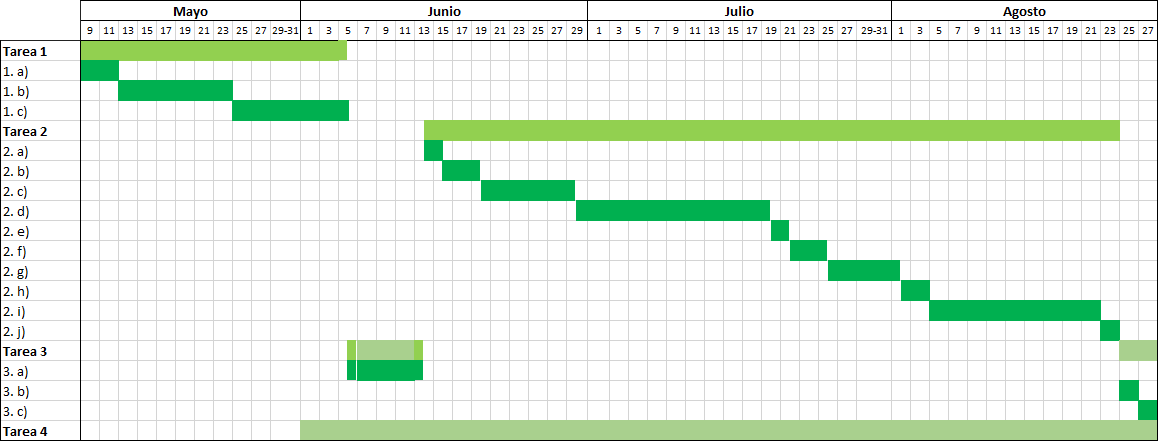
\includegraphics[width=1\textwidth]{figuras/gantt.png}
  \caption[Diagrama de \textit{Gantt} con la planificación de tareas]{Diagrama de Gantt con la planificación de tareas\\
  }
  \label{fig:diagramagantt}
\end{figure}


\section{Gestión de riesgos}

Todos estos procesos conllevan siempre asociado una posibilidad de que alguno de los equipos falle o se pueda perder algún tipo de información. Esto se trata en este apartado.

\subsection{Identificación de riesgos}

En los proyectos software hay cuatro tipos de riesgos:

\begin{itemize}

\item Riesgos técnicos: trata de riesgos relacionados con calidad, tecnologías utilizadas, requisitos, rendimiento, complejidad y fiabilidad.
\item Riesgos externos: los que tratan de factores externos, como proveedores, legislación, clientes, mercado y condiciones climáticas o localización.
\item Riesgos de la organización: los relacionados con financiación, recursos y dependencias entre las partes del proyecto
\item Riesgos de la dirección de proyectos: relacionados con la gestión de las tareas, la estimación de la duración de las mismas y las dependencias entre sí.

\end{itemize}

Se han listado varios fallos relacionados con este proyecto como, por ejemplo:

\begin{itemize}
\item Un fallo en el ordenador que haría desaparecer todo lo realizado hasta ahora, además del CSMS y de la base de datos. Este es de tipo técnico.
\item Cometer un error durante el proceso de desbloqueo y \textit{root} del smartphone que dejaría inservible el dispositivo. Es también de tipo técnico.
\item Puede haber problemas con la duración de las tareas si hay algún error en la asignación de tiempos. Es de tipo de dirección de proyectos.
\end{itemize}

\subsection{Análisis de riesgos}

Mediante el análisis de los riesgos identificados se recogerán datos sobre posibles retrasos, las respuestas a un riesgo y las formas de poder evitarlos:

\begin{itemize}
\item En el caso del ordenador un error en cualquier componente que no sea el disco duro sería salvable, dado que se pueden extraer con cierta facilidad los datos. Sin embargo, si el error está en el disco duro se perderá todo el trabajo. Por ello estos códigos referidos a las implementaciones se han ido subiendo a un repositorio de \textit{GitHub}. En caso de algún error se perdería el tiempo utilizado desde la última copia de seguridad.

En el caso del dispositivo móvil incluso en algunos momentos del proceso de \textit{root} se ofrece la opción de realizar copias de seguridad, algo que efectivamente se ha realizado. Se generaría en caso de algún error una pérdida económica al tener que reparar el dispositivo además del retraso temporal de tener que volver a desbloquearlo.

Los problemas en la gestión de duración de las tareas se pueden producir por problemas externos (suministro de clave de desbloqueo de smartphone por parte del fabricante) o internos (algún error en la programación que se haya visto tarde). El retraso sería el producido por la tardanza en resolver estos asuntos y una opción para poder evitarlo es el adelantar alguna otra tarea posterior en la medida de lo posible.

\end{itemize}

\section{Legislación y normativa}

En este apartado se tratará las leyes y normas que aplican sobre este trabajo. Por ello, se tratarán los delitos en los que incurriría una persona que realizase el proceso que se realizará en la prueba de concepto (\ref{Prueba de concepto}).

En internet y todas las tecnologías en las que este es una de sus bases una de las actuaciones que pueden causar un mayor daño es la suplantación de identidad. Este delito consiste en que una persona se haga pasar por otra para conseguir un beneficio. En este caso la suplantación se realiza mediante el robo de la etiqueta RFID de un usuario para recargar en su lugar, causando al usuario legítimo un perjuicio económico.

A pesar de que no existe un delito expreso para la suplantación de identidad en el Código Penal (\ref{CodigoPenal}), en el artículo 401 sí se recoge un fundamento jurídico (llamado \textit{usurpación de estado civil}) que sirve de base para dar a esta conducta la categoría de delito, castigado con una pena de prisión de seis meses a tres años. Por otro lado las disposiciones de los capítulos X, XI y XII sí aluden a la usurpación de identidad y la tipifican como delito. Ello lleva, en el marco jurídico actual, a ver que la suplantación de identidad es la suma de la usurpación de la identidad y la del estado civil.

Hay matices en función de cada caso de suplantación dependiendo de la acción realizada por el infractor y del alcance que se la ha causado a la víctima. En este caso la suplantación de la que trata de defender a los puntos de recarga este proyecto es la consistente al acceso del infractor a un servicio (recarga del coche eléctrico) de usuario haciéndose pasar por un usuario legítimo.

Para que el delito exista es necesario que el infractor haya obtenido rédito económico de la suplantación de identidad. En este caso se abriría un proceso penal contra el infractor que podría sufrir una condena de entre 1 y 4 años de prisión.

En caso de la víctima, esta deberá interponer una denuncia y llevarla a la entidad que da soporte al punto en el que ha recargado su vehículo para que esta restituya la cantidad robada.

Por otro lado, para poder obtener una indemnización por suplantación de identidad el afectado debe acudir a la vía civil, calculándose la cuantía de la indemnización según el alcance de los daños morales que observe el Tribunal.



\chapter{Solución}
\label{Solución}

En este apartado se explicará, de forma clara, tanto el sistema del que se dispone como de las soluciones que se han implementado para mejorar los aspectos de seguridad tratados en este trabajo. 

\section{Descripción de la solución}

Como se ha podido comprobar a lo largo de este trabajo, es relativamente sencillo el hecho de poder copiar la etiqueta de identificación de un dispositivo RFID para posteriormente poder replicarla, incluso con un smartphone con tecnología NFC implementada sin coste adicional.

Para poder reducir las posibilidades de ataque y complicar la posibilidad de reproducir este ataque, se han probado dos sistemas. 
El primero de ellos trata de un sistema de autenticación de doble factor (2FA), que es una forma de identificarse en el proceso con dos pasos en lugar de uno. Por ejemplo, en \cite{eados} se propone un sistema de autenticación MFA. En este trabajo el proceso será el siguiente:

\section{El proceso de análisis y desarrollo}

En primer lugar, se dispondría de una app para smartphone. Esta app actualizaría cada cierto tiempo una pantalla principal en la cual se verían durante otro tiempo los procesos de carga que esperan por el segundo paso de autenticación. En este trabajo la app se programa en el sistema operativo Android.

Para este segundo paso de autenticación podría haber varias opciones. Como se expresa en \cite{eatrece}, podría ser una identificación por biometría. También existen las posibilidades de realizar un doble paso de tarjetas RFID como se propone en \cite{eacinco}, en este caso tratándose de dos etiquetas adyacentes. Otra opción, que es la que se utiliza en este trabajo, se basaría en un código a recibir en el momento en el que se inicia el proceso de carga. Este código puede ser por SMS o por correo electrónico, eligiéndose el email en este caso porque no conllevaría un coste económico adicional.

Tras ello, se combinará este sistema con otro basado en una tarjeta basada en NFC variable, habiendo una comunicación previa entre la misma y el punto de recarga, registrando una semilla y jugando con la hora actual. Al no disponer de esa tecnología, se aprovechará la opción que nos proporciona la plataforma web que gestiona el CSMS de que un usuario pueda enviar una orden de inicio de recarga remota (RemoteStartTransaction), haciendo el CSMS todo el proceso de simulación de tarjeta NFC y de inicio de recarga.

Además, se tratará la configuración más segura para este punto de recarga, basándola en lo visto en el apartado anterior del protocolo OCPP. Esta configuración se realiza desde una plataforma disponible por parte del fabricante.

\subsection{Método basado en 2FA}

Este sistema cada vez es más habitual. Entre otros, es similar al utilizado en las aplicaciones bancarias, al de acceso a redes de empresas… En el caso de este trabajo funciona de la siguiente manera:

\begin{itemize}
\item En primer lugar, al tratar de iniciar la recarga el usuario asociado al identificador de la tarjeta que se trata de autorizar recoge el email asociado a este en la base de datos sobre la que trabaja el CSMS envía un correo electrónico con un código de 6 dígitos asociado al intento de inicio de recarga.
\item Posteriormente, en una app de Android programada para este trabajo y siempre que un usuario haya accedido se van realizando peticiones cada cierto tiempo. Estas peticiones consultan si hay alguna petición de inicio de recarga abierta por el propio usuario. En caso afirmativo, se verá en el listado de la pantalla principal de la app. 
\item Se pulsa sobre ella y se pide un código de seis dígitos para autorizarla. Tras introducirlo, se consulta si el código es correcto y, en caso afirmativo, se autoriza la recarga con el identificador de etiqueta que se ha pasado por el cargador o que se ha enviado de manera remota.
\end{itemize}

Para este método, al enviarse un paquete Authorize además de preguntar al CSMS si el usuario que trata de iniciar la recarga tiene autorización para ello o no, se crea una entrada en una tabla de la base de datos del CSMS para que, al autorizar en la aplicación, se cree la petición RemoteStartTransaction.


\subsection{Método basado en NFC con etiqueta aleatoria}

Este sistema se ha probado de manera simulada. Es decir, se ha diseñado un sistema para hacerlo todo desde el CSMS. En los sistemas actuales para la recarga del coche eléctrico, como ya se trató anteriormente en el trabajo, hay la opción de enviar las peticiones de inicio de recarga desde una app o una web que interactúa con el CSMS. Igualmente, se podrían implementar en una tarjeta o sistema basado en NFC. Este sistema es similar al que se utiliza para la apertura y cierre a distancia de las puertas de los coches. Con todo ello, este método funciona de la siguiente manera:

\begin{itemize}
\item En primer lugar, para iniciar la recarga, se realizaría un intercambio previo de una semilla sobre la cual se va a descifrar el identificador de etiqueta del cliente. Para el funcionamiento de ello se necesitaría implementar algún método de doble paso de claves por la pantalla del punto de recarga. Por ello en este ejemplo la semilla ya estaría guardada en el sistema CSMS y sólo se haría el paso de tarjeta con la semilla mezclada con la hora.
\item Este identificador de etiqueta se mezcla con la hora actual con el siguiente formato: YYYYMMDDhhmmss.
\item Con ello, se envía el inicio de recarga. Al hacerlo de manera combinada con la autorización en doble factor, se realiza el proceso con la app de Android programada para este trabajo y, tras hacerse la comprobación de que, efectivamente, el usuario que recarga es el que se espera, ya se inicia correctamente el proceso de recarga.
\end{itemize}

Para este método no hay que hacer ningún cambio más en el sistema aparte de la simulación de esta tarjeta basada en NFC.



\subsection{Diseño}

Para implementar esto se requiere, en primer lugar, un sistema como el explicado en el capítulo \ref{Arquitectura de un sistema basado en OCPP}. Tras ello, se añadirán las herramientas creadas para la mejora de la seguridad, las cuáles no requieren en esta prueba un aumento de la estructura del sistema. En un caso real sí se añadiría una tarjeta NFC.

\subsubsection{Diseño de sistema}

En primer lugar, relacionado con lo se explicó, se utilizarán los siguientes elementos.

\begin{itemize}
\item Un ordenador que dará soporte tanto al CSMS como a la base de datos.
\item Un punto de recarga.
\item Un smartphone para iniciar recargas.
\item Una tarjeta con una etiqueta RFID para las simulaciones previas y la prueba de concepto.
\item Una manguera para simular una recarga.
\end{itemize}

Para esta simulación se conectarán tanto ordenador (CSMS y BD) como punto de recarga a la misma red y no siendo evidentemente necesario que los demás equipos estén conectados.

El CSMS utilizado se llama \textit{Planet Charger}. Es un servidor web mediante el cual, interactuando con la base de datos, se pueden realizar las siguientes acciones.

\begin{itemize} 
\item Un resumen de los datos de recargas.
\item Registrar y editar los cargadores conectados al CSMS y algunos de sus datos.
\item Registrar y editar los usuarios con permiso para recargar y sus datos.
\item Disponer de un histórico de recargas realizadas en los cargadores conectados al CSMS.
\item Disponer de un histórico de los paquetes y peticiones intercambiadas entre cargadores y CSMS.
\item Otros enlaces de interés como gráficas, tarifas...
\end{itemize}


En el caso de este trabajo lo interesante son tanto los cargadores conectados a los CSMS, los permisos de los usuarios y el registro de las recargas.

Este servidor web funciona con los lenguajes HTML, PHP, CSS y JavaScript.
\begin{itemize} 
\item HyperText Markup Language (HTML) es el componente más básico de la Web, ya que define el significado y la estructura del contenido web. Se combina con otras tecnologías para describir la visualización de una página web (CSS) o comportamientos (JavaScript).
\item Hypertext Preprocessor (PHP) es un lenguaje de código abierto adecuado para el desarrollo web y que puede ser incrustado en HTML. Se utiliza la versión 7.2.5.
\item Cascading Style Sheets (CSS) es el lenguaje de estilos utilizado para describir la presentación de documentos HTML.
\item JavaScript (JS) es un lenguaje de programación ligero, interpretado, o compilado justo-a-tiempo (just-in-time) conocido mayormente como un lenguaje de scripting (secuencias de comandos) para páginas web.
\end{itemize}

El servidor web que se utiliza es Internet Information Services (IIS). Este convierte a un ordenador en un servidor web tanto para Internet como para intranet, es decir, que en los equipos que tienen este servicio instalado se podrían publicar páginas web de forma local y de forma remota. Se basa en este caso en un módulo PHP. La versión que se utiliza en este trabajo es la 10.0.

La base de datos se basa en MariaDB. Este es un sistema de gestión de bases de datos derivado de MySQL con licencia GPL (General Public License). Se utiliza la versión 10.9.

Como se ha descrito anteriormente, la comunicación con el punto de recarga se realiza a través de WebSocket y utilizando el protocolo de comunicación OCPP 1.6.

Por otra parte, desde el propio ordenador y para facilitar el trabajo, se utiliza un gestor de puntos de recarga. Este puede ver los EVSE conectados a la misma red del ordenador en el que se ejecuta. La aplicación se llama \textit{Ace Service Installer}.

Para las recargas se simulará una tarjeta NFC en lenguaje también PHP. 

Se diseñará una app para sistemas operativos Android para completar la autenticación 2FA. Para ello se utiliza Android Studio y el lenguaje de programación Java.


\subsubsection{Diseño detallado}

En este apartado se describirán los aspectos más visuales del sistema y funcionamiento y, posteriormente, se tratarán las implementaciones realizadas para llevar cumplir los requisitos propuestos en el trabajo.

En primer lugar, el servicio web base utilizado, \textit{Planet Charger}, dispone en su inicio de una pantalla para acceder.

\begin{figure}[H] 
\centering
  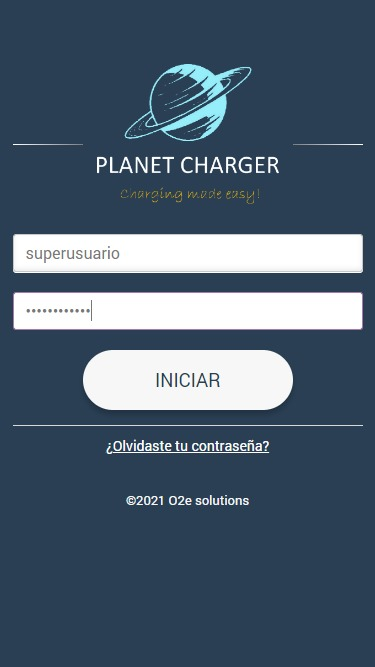
\includegraphics[width=.5\textwidth]{figuras/design1.png}
  \caption[Pantalla de acceso de la web]{Pantalla de acceso de la web\\
  }
  \label{fig:design1}
\end{figure}

Tras acceder a la plataforma, hay un menú lateral. En ese menú lateral los botones de \textit{Datos}, \textit{Usuarios}, \textit{Plazas}, \textit{Sesiones de recarga} y \textit{Comunicación}.

\begin{figure}[H] 
\centering
  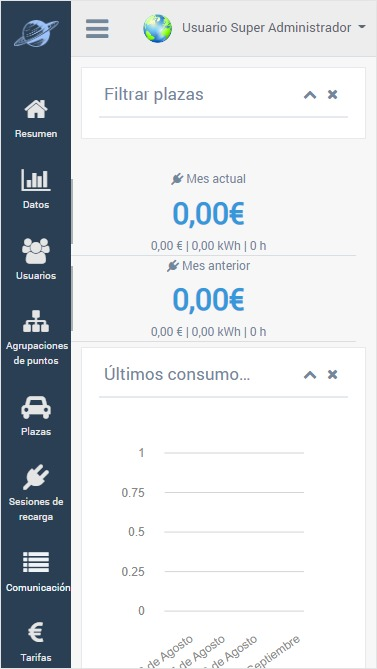
\includegraphics[width=.5\textwidth]{figuras/design2.png}
  \caption[Pantalla principal de la web]{Pantalla principal de la web\\
  }
  \label{fig:design2}
\end{figure}

Si se accede en el botón \textit{Usuario} se dispone de un listado de los usuarios registrados en la aplicación. Al editar un usuario se ven varios datos. En el caso de este trabajo, solamente nos interesan \textit{e-mail} y \textit{Semilla de UID de tarjeta}. El primero para la autenticación doble factor y el segundo para la tarjeta NFC, en este caso simulada.

\begin{figure}[H] 
\centering
  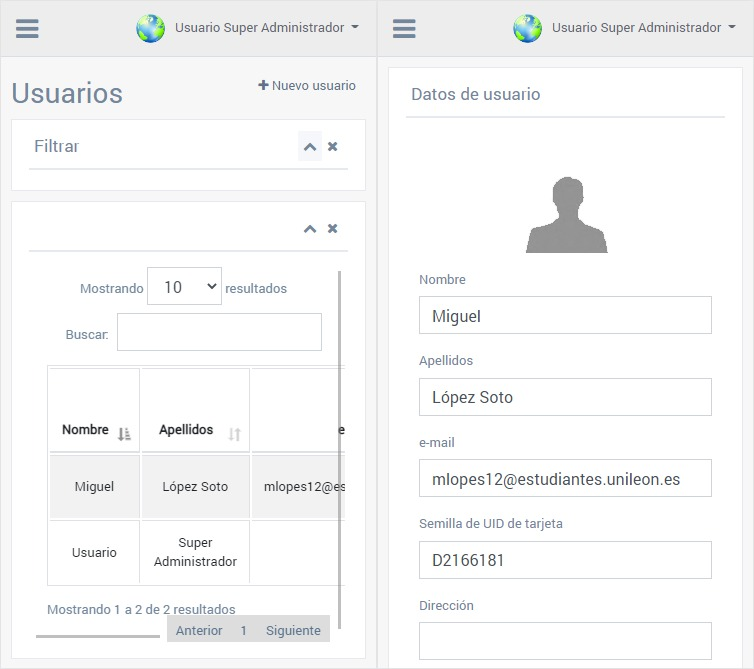
\includegraphics[width=1\textwidth]{figuras/design3.png}
  \caption[Pantallas de usuario]{Pantallas de usuario\\
  }
  \label{fig:design3}
\end{figure}

Tras este, hay otros apartados de interés de la web. En \textit{Plazas} hay dos enlaces, uno que lleva a un listado para editar los puntos de recarga y otro para comprobar su estado y dos botones, uno realizar algún tipo de operaciones sobre ellos, como reiniciarlos o realizar inicios y fines de recargas, y otro para consultar y cambiar la configuración general del EVSE.


\begin{figure}[H] 
\centering
  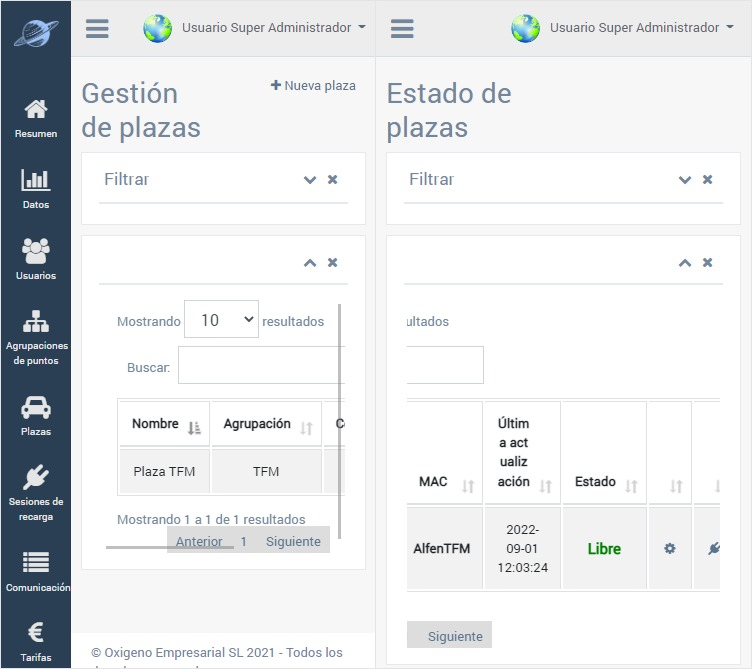
\includegraphics[width=1\textwidth]{figuras/design4.png}
  \caption[Pantallas referidas a puntos de recarga]{Pantallas referidas a puntos de recarga\\
  }
  \label{fig:design4}
\end{figure}

Además del botón \textit{Sesiones de recarga}, donde se encuentran las cargas realizadas, se dispone de otro botón llamado \textit{Comunicación}. En el enlace \textit{Eventos} se dispone de los paquetes enviados por el punto de recarga. Y en respuestas se ven las respuestas del sistema a estos paquetes enviados por el punto.

\begin{figure}[H] 
\centering
  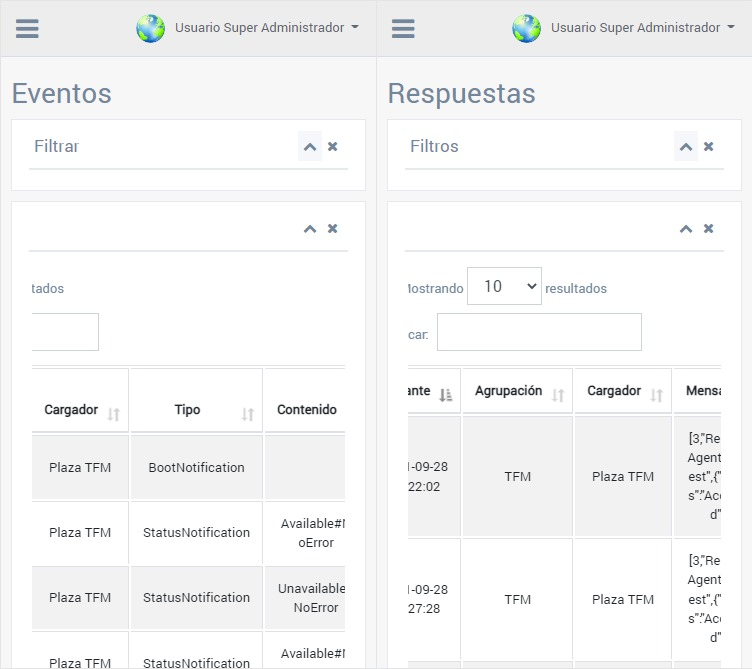
\includegraphics[width=1\textwidth]{figuras/design5.png}
  \caption[Pantallas referidas a las comunicaciones con los puntos de recarga]{Pantallas referidas a las comunicaciones con los puntos de recarga\\
  }
  \label{fig:design5}
\end{figure}

Para la ejecución de la autenticación 2FA se ha implementado un pequeño módulo en el que se reciben las peticiones de inicio de proceso de recarga generadas para poder confirmarlas. 

En este caso no se ha profundizado dado que se trata de un modelo simulado. Sin embargo, gran parte de las compañías que dan soporte a la recarga del vehículo del coche eléctrico disponen de aplicaciones, tanto en Android como en iOs, para realizar los procesos y controles que se hacen desde la app, al menos en la parte de llevar el control de procesos de recarga y de histórico de recargas del propio usuario. Por ello este módulo que se ha implementado como una entidad independiente podría integrarse sin problemas en una app de una compañía eléctrica.

En primer lugar, al igual que en el anterior sistema, se dispone de una pantalla de inicio de acceso en la que se deben introducir los mismos datos que en la web.

\begin{figure}[H] 
\centering
  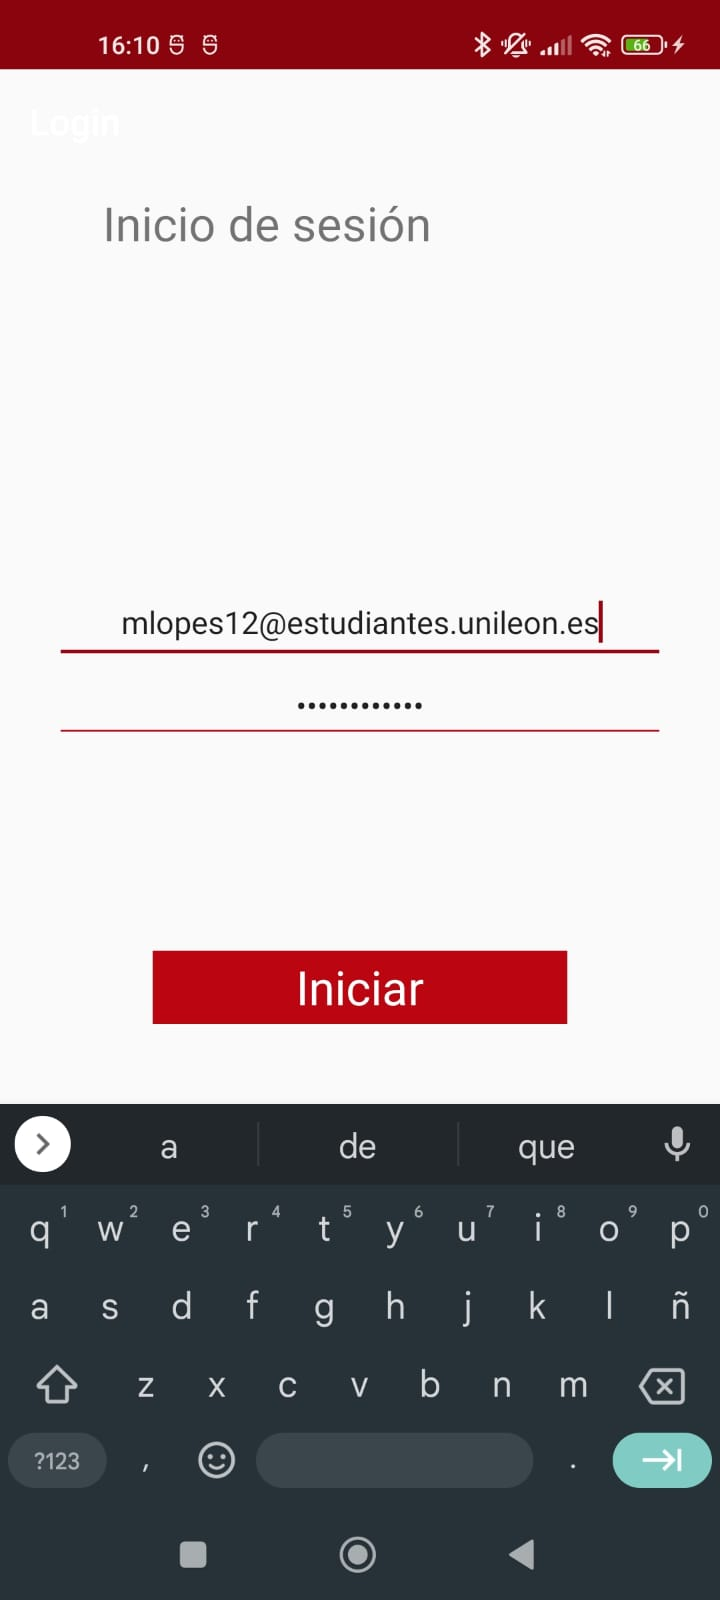
\includegraphics[width=0.5\textwidth]{figuras/design6.png}
  \caption[Pantalla principal de acceso de la app]{Pantalla principal de acceso de la app\\
  }
  \label{fig:design6}
\end{figure}

Al acceder de forma correcta, se percibe el listado de recargas a finalizar su autenticación. Habitualmente sólo se verá una dado que lo habitual es un usuario cargando con un vehículo.

\begin{figure}[H] 
\centering
  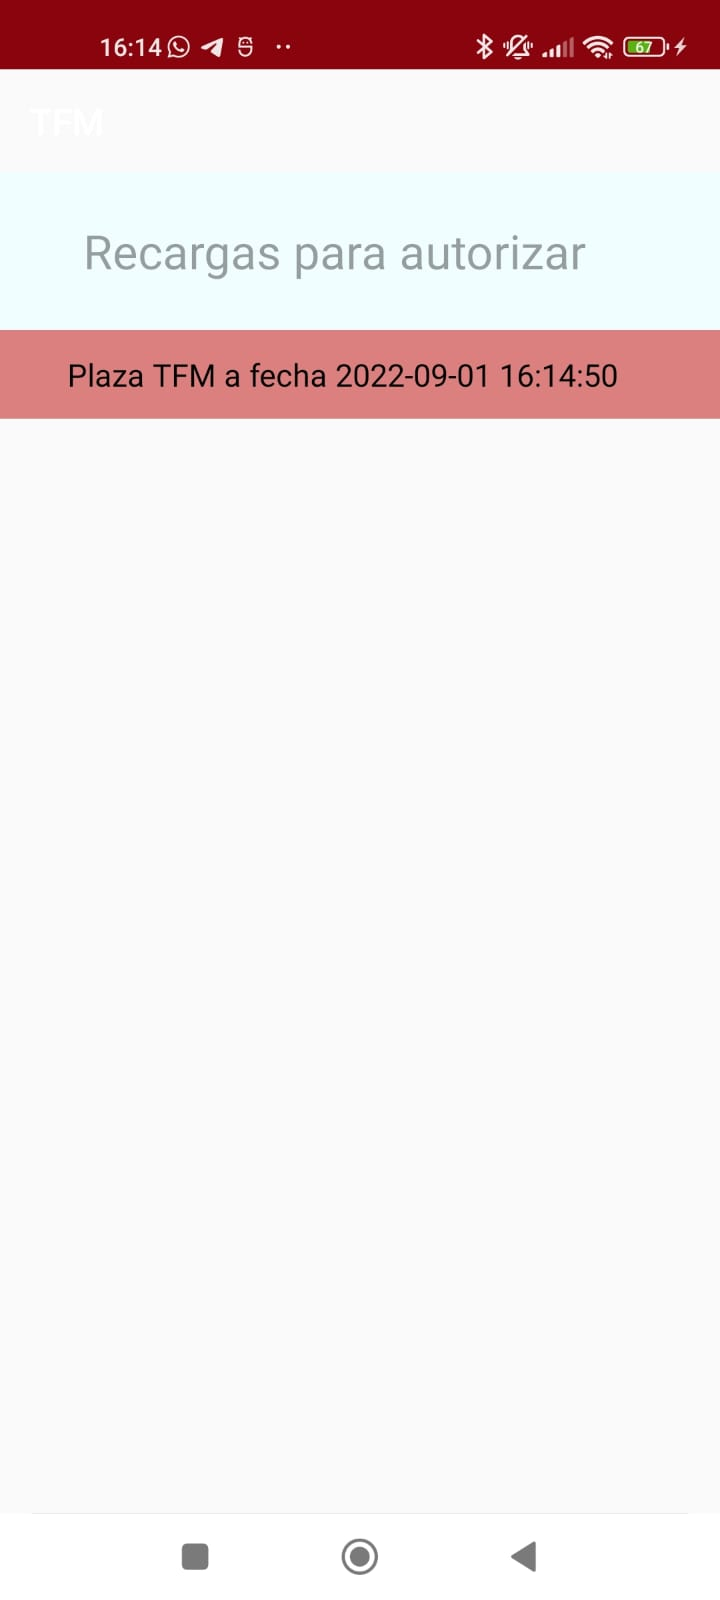
\includegraphics[width=0.5\textwidth]{figuras/design7.png}
  \caption[Pantalla con el listado de cargas a confirmar]{Pantalla con el listado de cargas a confirmar\\
  }
  \label{fig:design7}
\end{figure}

Tras confirmarlo, se ve la pantalla en la que hay que insertar el código recibido por correo electrónico al iniciar el proceso de recarga.

\begin{figure}[H] 
\centering
  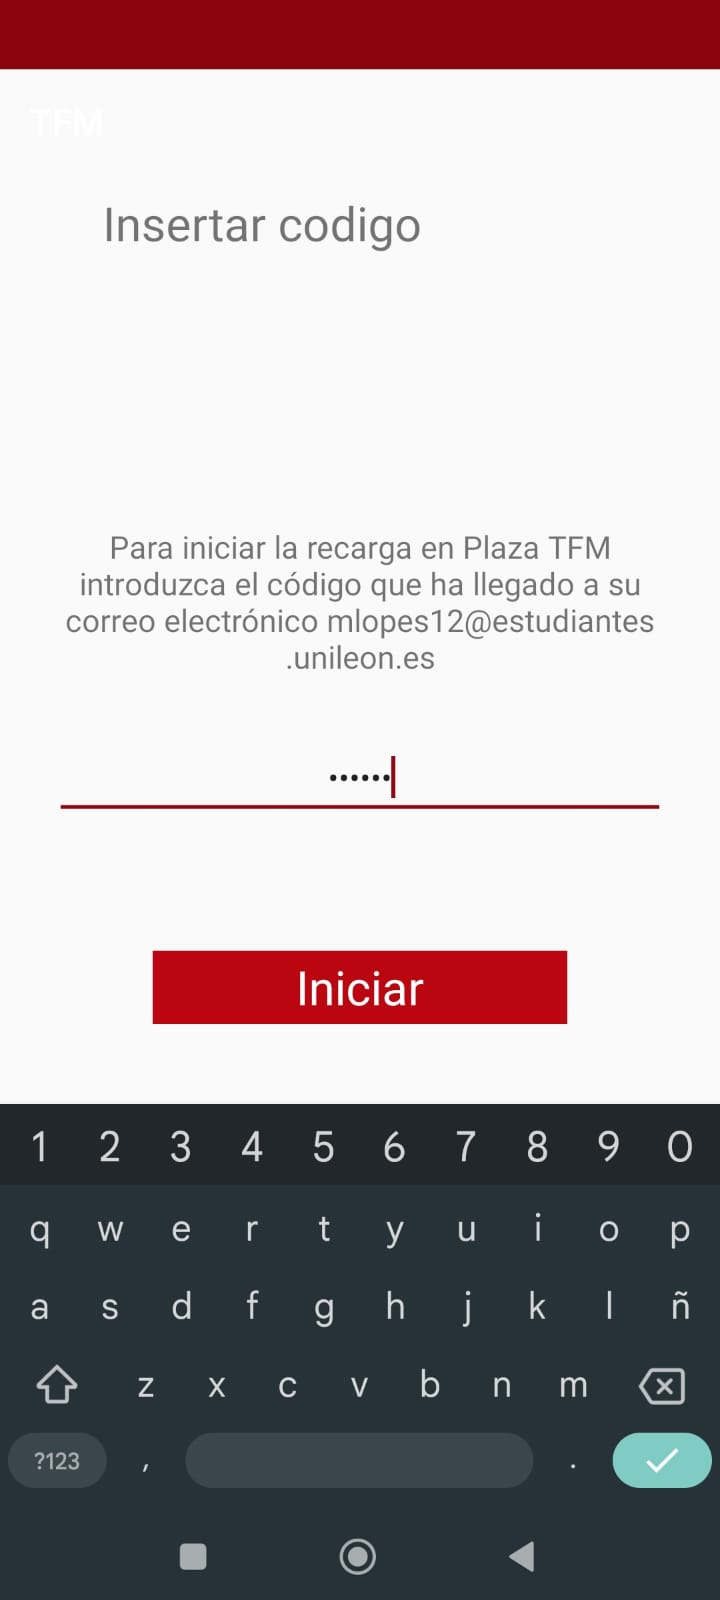
\includegraphics[width=0.5\textwidth]{figuras/design8.png}
  \caption[Pantalla en la que introducir el código de confirmación de inicio de recarga]{Pantalla en la que introducir el código de confirmación de inicio de recarga\\
  }
  \label{fig:design8}
\end{figure}

Como se ve, todo lo que hace este sistema, al igual que la app de Android es interactuar para añadir, editar y eliminar datos en la base de datos e iniciar o parar recargas.


\subsection{Implementación}

En este apartado se tratan los dos sistemas programados en este apartado, comparando los procesos actuales con los resultantes tras estos cambios. El código de los mismos se podrá encontrar en los anexos de este trabajo.

Para la realización de la autenticación 2FA se han realizado los siguientes pasos:
\begin{itemize}
\item Lo primero es la creación una tabla en particular en la base de datos con los campos:
\begin{itemize}
\item \textit{id\_authorization} (identificador único de la solicitud de inicio de recarga)
\item \textit{id\_plaza} (identificador único de la plaza en la que se pretende iniciar recarga)
\item \textit{idTag} (etiqueta de identificación con la que se pretende iniciar recarga)
\item \textit{codigo} (código que se envía por email al usuario al que está asociado la tarjeta y que este tiene que introducir en la app para confirmar el inicio de recarga)
\item \textit{fecha} (fecha de solicitud del inicio de recarga)
\item \textit{validez} (tiempo en segundos de validez de la solicitud de inicio de recarga)
\item \textit{id\_individuo} (identificador único del individuo que pretende iniciar recarga)
\item \textit{autorizada} (indica si se ha confirmado la solicitud de inicio o no)
\item \textit{idTagCharge} (etiqueta de identificación con la que se inicia la recarga que es distinta a la de la tarjeta para evitar la posibilidad de que con la misma etiqueta que se inicia carga se pueda detener)
\end{itemize}
\item Posteriormente, tanto en la función que interpreta los paquetes \textit{Authorize} como en el \textit{RemoteStopTransaction} añadir una función que introduzca una entrada en la tabla y que envíe un correo con un código PIN para realizar la autorización 2FA.
\item La app, programada en Windows mediante \textit{Android Studio}, realiza constantemente una consulta asíncrona a la base de datos con un identificador de usuario para ver cuáles son las recargas pendientes de la doble autorización.
\item La app envía el código al servicio web, que comprueba si es correcto y contesta a la app. Si es correcto, se inicia la recarga. En caso contrario llegará un aviso de que es incorrecto.
\item Para detener la recarga simplemente se debe realizar un paso de tarjeta o hacerlo desde la web.
\end{itemize}

\begin{figure}[H] 
\centering
  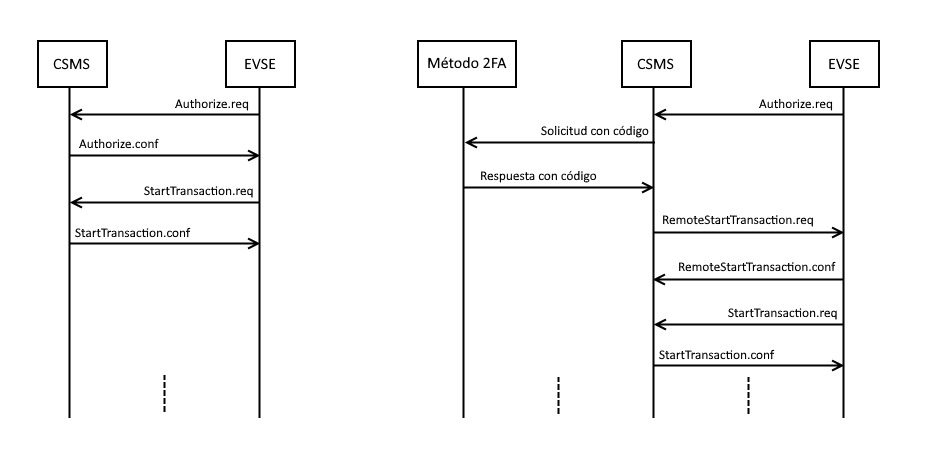
\includegraphics[width=1\textwidth]{figuras/diagrama2faauthorize.png}
  \caption[Diagrama de flujo del funcionamiento del protocolo OCPP 1.6 (izquierda) y añadiendo la autenticación 2FA (derecha) iniciando el proceso de recarga con una tarjeta]{Diagrama de flujo del funcionamiento del protocolo OCPP 1.6 (izquierda) y añadiendo la autenticación 2FA (derecha) iniciando el proceso de recarga con una tarjeta\\
  }
  \label{fig:diagrama2fa1}
\end{figure}

\begin{figure}[H] 
\centering
  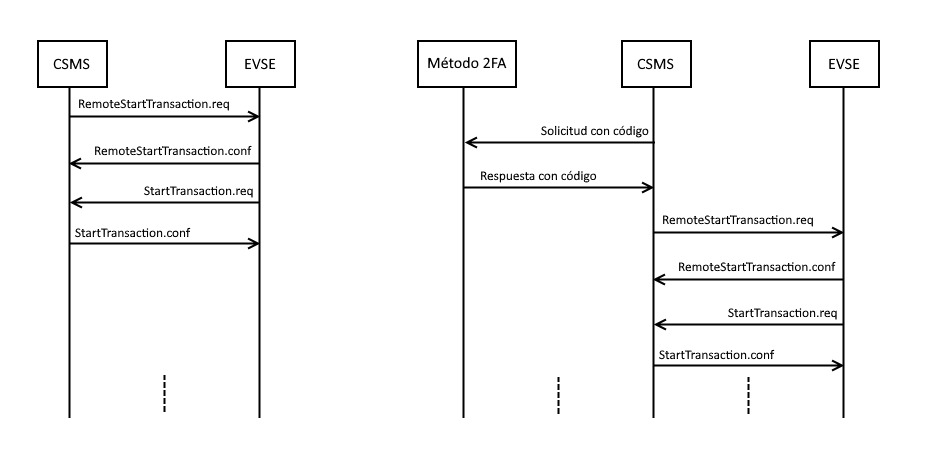
\includegraphics[width=1\textwidth]{figuras/diagrama2farst.png}
  \caption[Diagrama de flujo del funcionamiento del protocolo OCPP 1.6 (izquierda) y añadiendo la autenticación 2FA (derecha) iniciando el proceso de recarga desde el CSMS]{Diagrama de flujo del funcionamiento del protocolo OCPP 1.6 (izquierda) y añadiendo la autenticación 2FA (derecha) iniciando el proceso de recarga desde el CSMS\\
  }
  \label{fig:diagrama2fa2}
\end{figure}


Para la simulación de la tarjeta NFC aleatoria:
\begin{itemize}
\item Se crea una función, la cual genera, a partir de una semilla, un número variable multiplicándola con la fecha y hora actuales en segundos.
\begin{itemize}
\item La semilla hexadecimal sobre la que se va a calcular la etiqueta se pasa a decimal (para las simulaciones posteriores se recoge la etiqueta de una tarjeta RFID).
\item Se toma toda la fecha actual en segundos.
\item Los dos valores anteriores se multiplican y se convierten a hexadecimal.
\item Finalmente se recogen los catorce caracteres más significativos y, en caso de que haya menos de catorce, se añaden a la derecha tantos ceros como se necesiten hasta cubrir los catorce.
\end{itemize}
\item En caso de que se detenga con la tarjeta se hace la misma generación a partir de la semilla en el \textit{Authorize}, pero en este caso se añade la función a la comprobación. Al no poder pararse con una tarjeta distinta a la que inició recarga (eso sólo pasa cuando se produce una reserva antes de iniciar la recarga) se envía un \textit{RemoteStopTransaction} siempre y cuando la tarjeta esté autorizada. En caso de que sea un \textit{RemoteStopTransaction} desde la web no hay nada que modificar ya que no necesita de la etiqueta para detener la recarga.
\end{itemize}
\begin{figure}[H] 
\centering
  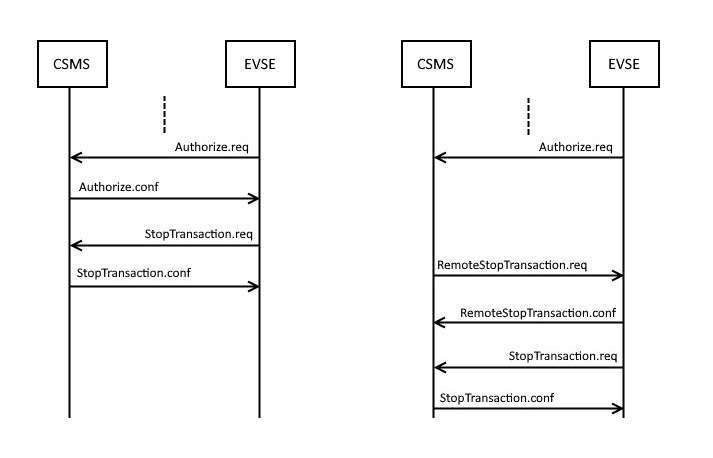
\includegraphics[width=1\textwidth]{figuras/diagramaNFCvariable.png}
  \caption[Diagrama de flujo del funcionamiento del protocolo OCPP 1.6 (izquierda) y añadiendo una etiqueta variable (derecha) finalizando el proceso de recarga con una tarjeta]{Diagrama de flujo del funcionamiento del protocolo OCPP 1.6 (izquierda) y añadiendo una etiqueta variable (derecha) finalizando el proceso de recarga con una tarjeta\\
  }
  \label{fig:diagramanfc}
\end{figure}

Y, finalmente, el resultado definitivo se produce aplicando ambos criterios de forma simultánea. Dado que afectan a partes distintas del proceso no se modifican el uno al otro.

Sin embargo, para la simulación en los \textit{Authorize} se hace una simulación modificando la etiqueta de una tarjeta no variable. Con ella se puede simular el comportamiento de una tarjeta NFC en los procesos que inicia el EVSE. Para los procesos que inicia el servicio web del CSMS esta simulación sería la implementación en código definitiva.







\subsection{Pruebas}
\label{Pruebas}

Las pruebas realizadas para comprobar esta problemática y su solución son las siguientes:

\begin{itemize}
\item En primer lugar una prueba de concepto. Esta se realizará mediante la lectura de una etiqueta RFID por parte de un smartphone y la posterior emisión de la misma mediante la tecnología NFC del propio dispositivo.
\item Finalmente, tras la implementación de las soluciones, se realizarán tres pruebas concretas:
\begin{itemize}
\item La primera de ellas es la prueba de un sistema de autenticación de doble factor (2FA) en la que el usuario se autorizará mediante una app de Android y un código que llega al correo electrónico de su cuenta de usuario en la plataforma tras tratar de iniciar la recarga. Esta parte securiza el inicio de la recarga.
\item La segunda es la introducción de una etiqueta RFID variable mediante NFC. Es decir, al iniciar la recarga se utilizará un número de tarjeta para autorizar al usuario, a la carga se le asociará otra etiqueta aleatoria para no poder detener la recarga con la primera etiqueta (para proteger de mayor forma ante las posibles suplantaciones) y para finalizar la recarga se utilizará una tercera etiqueta. La primera y la tercera se generarán a través de una semilla y el uso de la fecha y la hora, pudiendo ser otras opciones para futuros desarrollos un contador o algún otro valor. Este método securiza tanto el inicio como el fin de la recarga, pero en mayor medida el final de la misma.
\item En último lugar se unirán ambos métodos para conseguir una protección mayor para todo el proceso.

\end{itemize}

\end{itemize}




\chapter{Evaluación}
\label{Evaluación}

El objetivo de este trabajo era aumentar la seguridad en uno de los puntos del proceso de la recarga del coche eléctrico más vulnerables: la autorización del usuario. Al utilizarse un sistema con una simple etiqueta de identificación RFID, esta es sencilla de robar (como se vio en \ref{Prueba de concepto}). Esto propicia el ataque de suplantación de identidad, en la que otro usuario se haría pasar por el usuario autorizado para recargar sin su consentimiento.

Para ello se han propuesto las dos soluciones tratadas. La primera, autenticación 2FA, está referida al software, por lo que se podría añadir con los sistemas actuales, dado que solo añadiría un punto intermedio en el proceso de inicio de recarga. Para la segunda se necesitaría una mayor infraestructura para comprender las tarjetas variables,  que estas de algún modo dispusieran de un temporizador o algún tipo de contador para reproducir el sistema y que el punto de recarga fuese capaz de comprender de algún modo esta información.

\section{Proceso de evaluación}

Se desarrollarán, como ya se vio en \ref{Pruebas}, varios procedimientos de inicio y fin de carga, así como una prueba de concepto del robo de los datos de una etiqueta RFID mediante un smartphone.

\subsection{Forma de evaluación}

En primer lugar, en la prueba de concepto, para considerar un funcionamiento correcto de la misma se deberá conseguir iniciar recarga acercando el smartphone (con la tecnología NFC activada) por el punto de recarga y conseguir iniciar una recarga.

En los casos posteriores, diseñados para evitar este problema, se han tratado de realizar varias suplantaciones de identidad, utilizando la etiqueta de la tarjeta con permiso en ambas. Con el funcionamiento actual del protocolo OCPP en ambos casos debería producirse esta suplantación, iniciando y deteniendo recarga. Además deberán iniciarse y finalizarse correctamente los procesos de recarga probados.

Para poder determinar si la solución es correcta se debe hacer el mismo proceso de robo de tarjeta y ver que en uno de los casos no inicia la recarga y en el otro no se detiene. Viendo esto y no observando ninguna pérdida de funcionalidad se deberían dar por buenas ambas soluciones.

\subsection{Casos de prueba}

En este apartado se diseminan tanto la prueba de concepto como las soluciones implementadas para evitar que mediante esta prueba se consiga robar una tarjeta NFC. Además, antes de ello, hay que realizar una configuración previa del punto de recarga mediante la una aplicación del fabricante destinada para ello. Esta configuración seguiría permitiendo el robo de tarjeta pero elimina bastantes opciones de ello.

\subsubsection{Prueba de concepto}
\label{Prueba de concepto}

La prueba de concepto o PoC (Proof of Concept) es la implementación de un método o de una idea que trata de verificar que el concepto o teoría en cuestión es susceptible de ser explotada de una forma realista.

En este apartado se describirá un posible caso real de robo del identificador de una tarjeta de fidelización de un cliente y los pasos seguidos para el mismo. Se dispone de un smartphone modelo Xiaomi Redmi Note 8T, mediante el cuál se procederá a leer una tarjeta con una etiqueta RFID. Desde ese mismo teléfono móvil se simulará la emisión del mismo código para que, con el propio móvil se pueda recargar como si fuese el usuario al cuál se le han robado los datos.

Es necesario conseguir \textit{rootear} en primer lugar el dispositivo dado que es la única opción de simular la emisión de códigos de tarjetas distintos a los generados por el propio dispositivo. Este es el proceso que permite a los usuarios de dispositivos Android obtener algunos privilegios para modificar algunas funciones que vienen por defecto en estos dispositivos.

Para ello, en el caso del dispositivo que se va a utilizar para esta prueba se deben activar, en primer lugar, las opciones de desarrollador. Se hace en la pantalla de ajustes, en el apartado \textit{Mi dispositivo}, pulsando siete veces en \textit{Versión de MIUI}.


\begin{figure}[H] 
\centering
  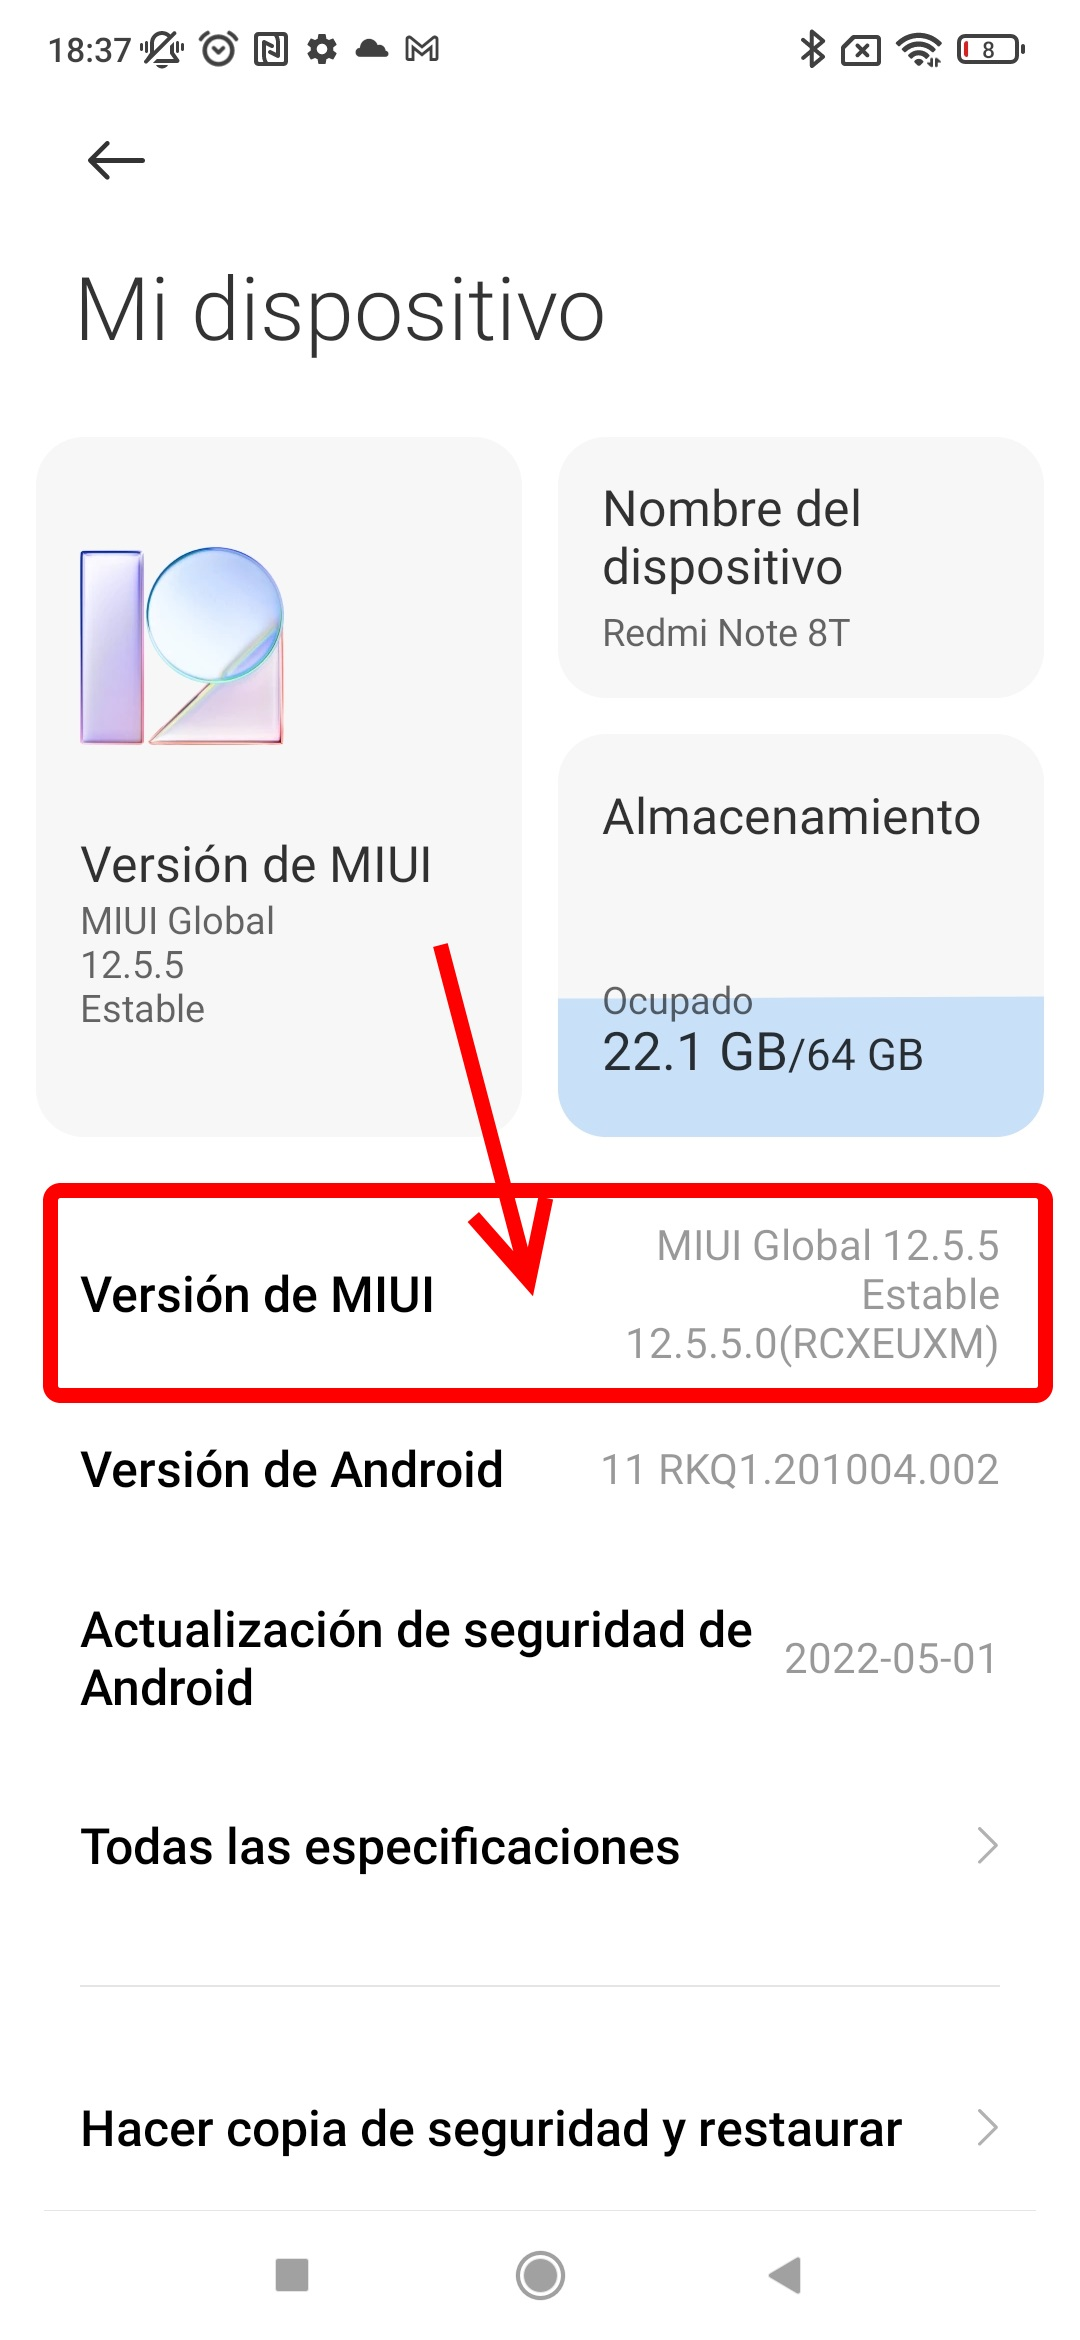
\includegraphics[width=0.4\textwidth]{figuras/root1.png}
  \caption[Pantalla de \textit{Mi Dispositivo}]{Pantalla de \textit{Mi Dispositivo}\\
  }
  \label{fig:root1}
\end{figure}

Posteriormente se debe desbloquear el \textit{bootloader} (gestor de arranque) para poder instalar una \textit{ROM} (versiones modificadas de Android) o rootear el dispositivo, y para ello se deben en primer lugar activar tanto la \textit{depuración USB} como el \textit{desbloqueo OEM}. Esto se hace nuevamente en los ajustes del dispositivo dentro de las opciones de \textit{Ajustes adicionales} en los botones \textit{Opciones de desarrollador} y \textit{desbloqueo de OEM}. Se activan y dentro del desbloqueo OEM pedirá una cuenta de usuario del fabricante Xiaomi y disponer de una tarjeta SIM para continuar el proceso.

\begin{figure}[H] 
\centering
  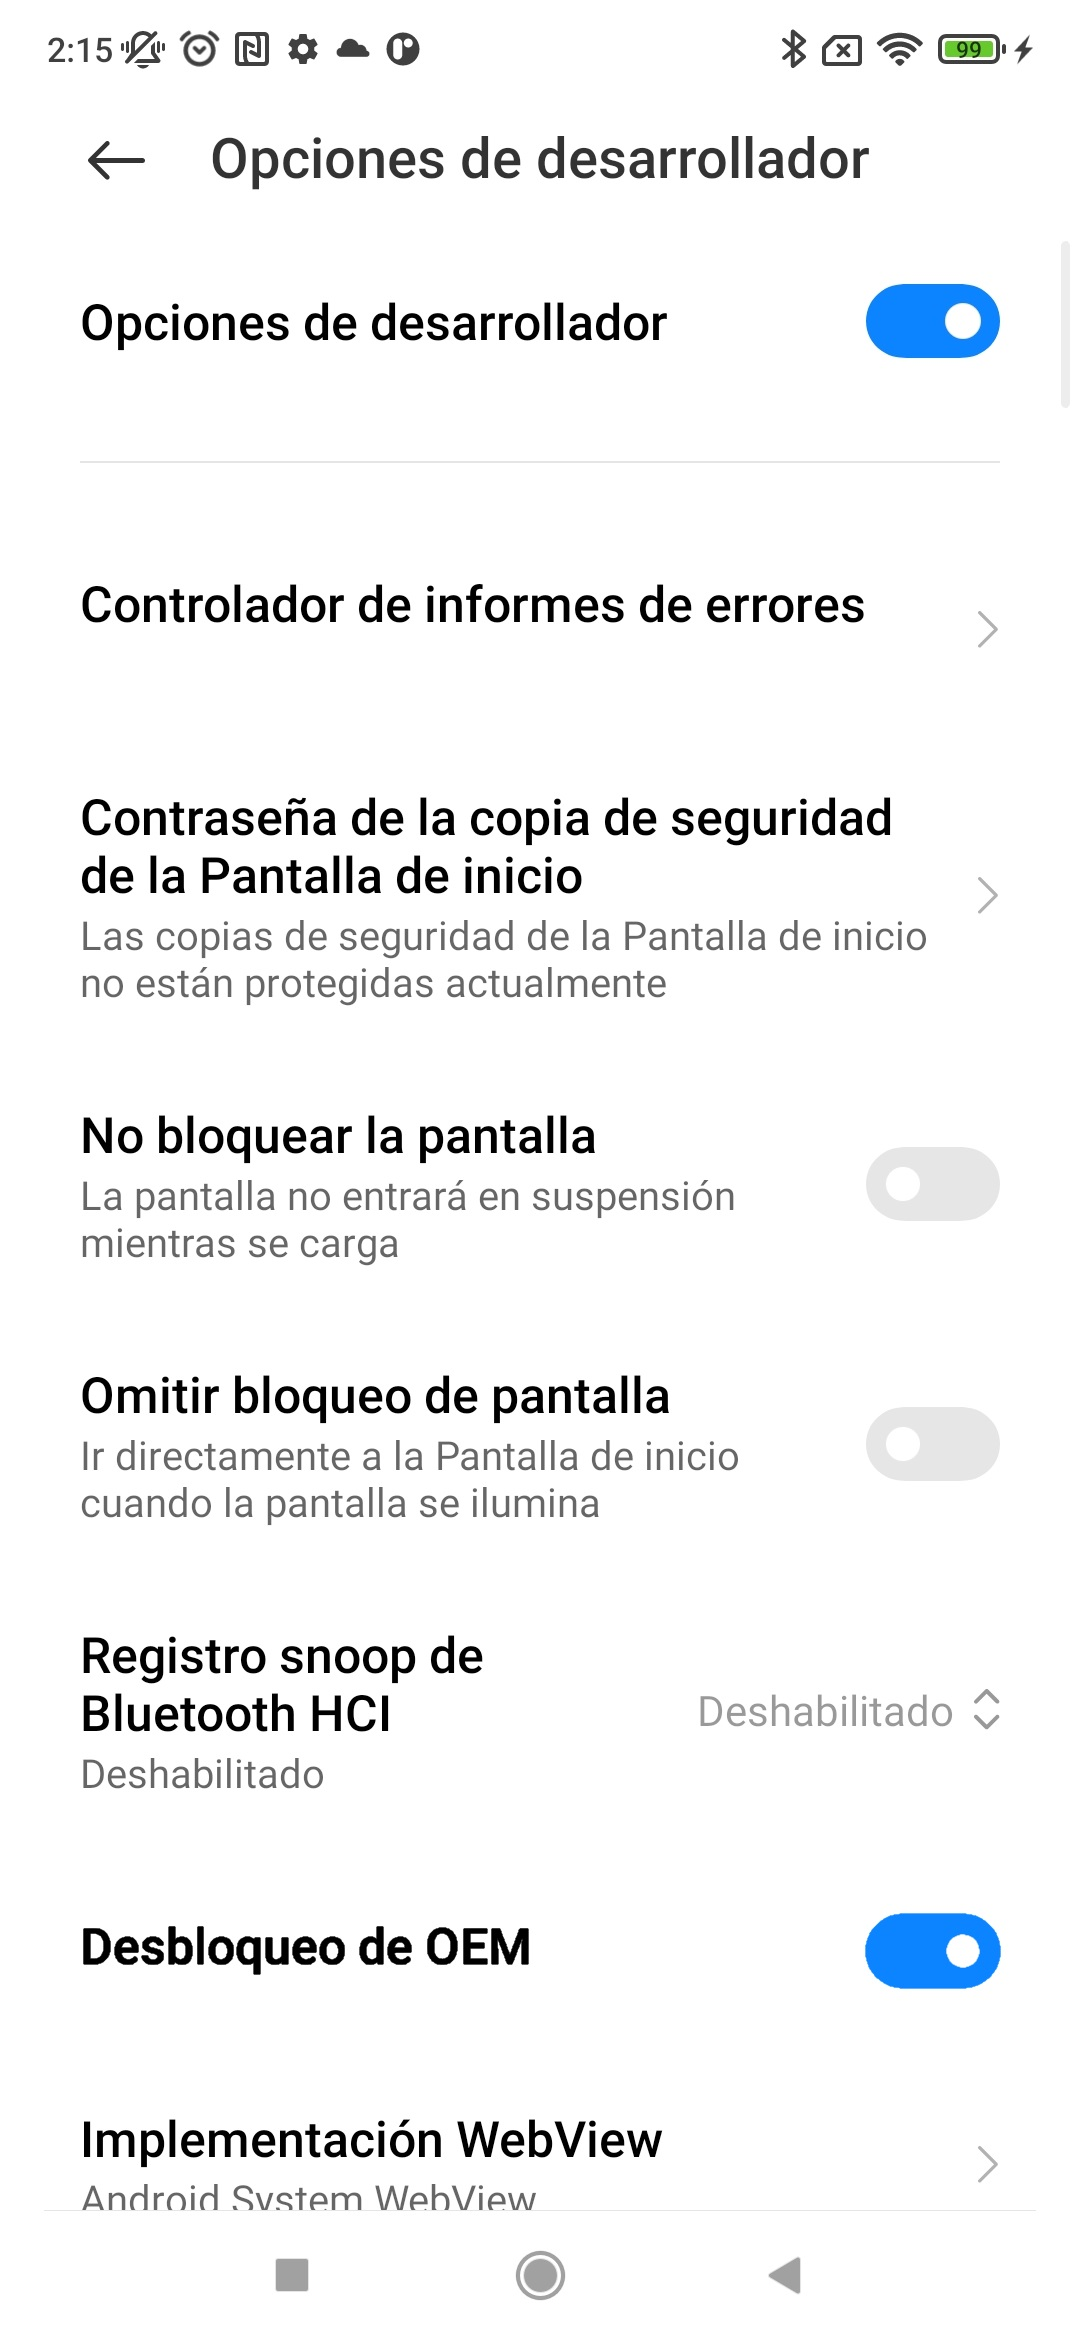
\includegraphics[width=0.4\textwidth]{figuras/root2.png}
  \caption[Pantalla de \textit{Opciones de desarrollador}]{Pantalla de \textit{Opciones de desarrollador}\\
  }
  \label{fig:root2}
\end{figure}

Para realizar este desbloqueo se necesita disponer de un ordenador con sistema operativo Windows, dado que el programa que permite realizar este proceso (\textit{Mi Unlock}) funciona en este tipo de sistemas, además de un cable USB para conectar el smartphone al mismo.

Se debe, por tanto, instalar ese programa e iniciar sesión en él con la cuenta de Xiaomi del propio dispositivo. Se apaga el teléfono y se enciende pulsando tanto el botón de encendido como el de volumen arriba para iniciarlo en un modo llamado \textit{fastboot}. Se conecta al ordenador y se espera que el botón \textit{Unlock} se sitúe en verde.

\begin{figure}[H] 
\centering
  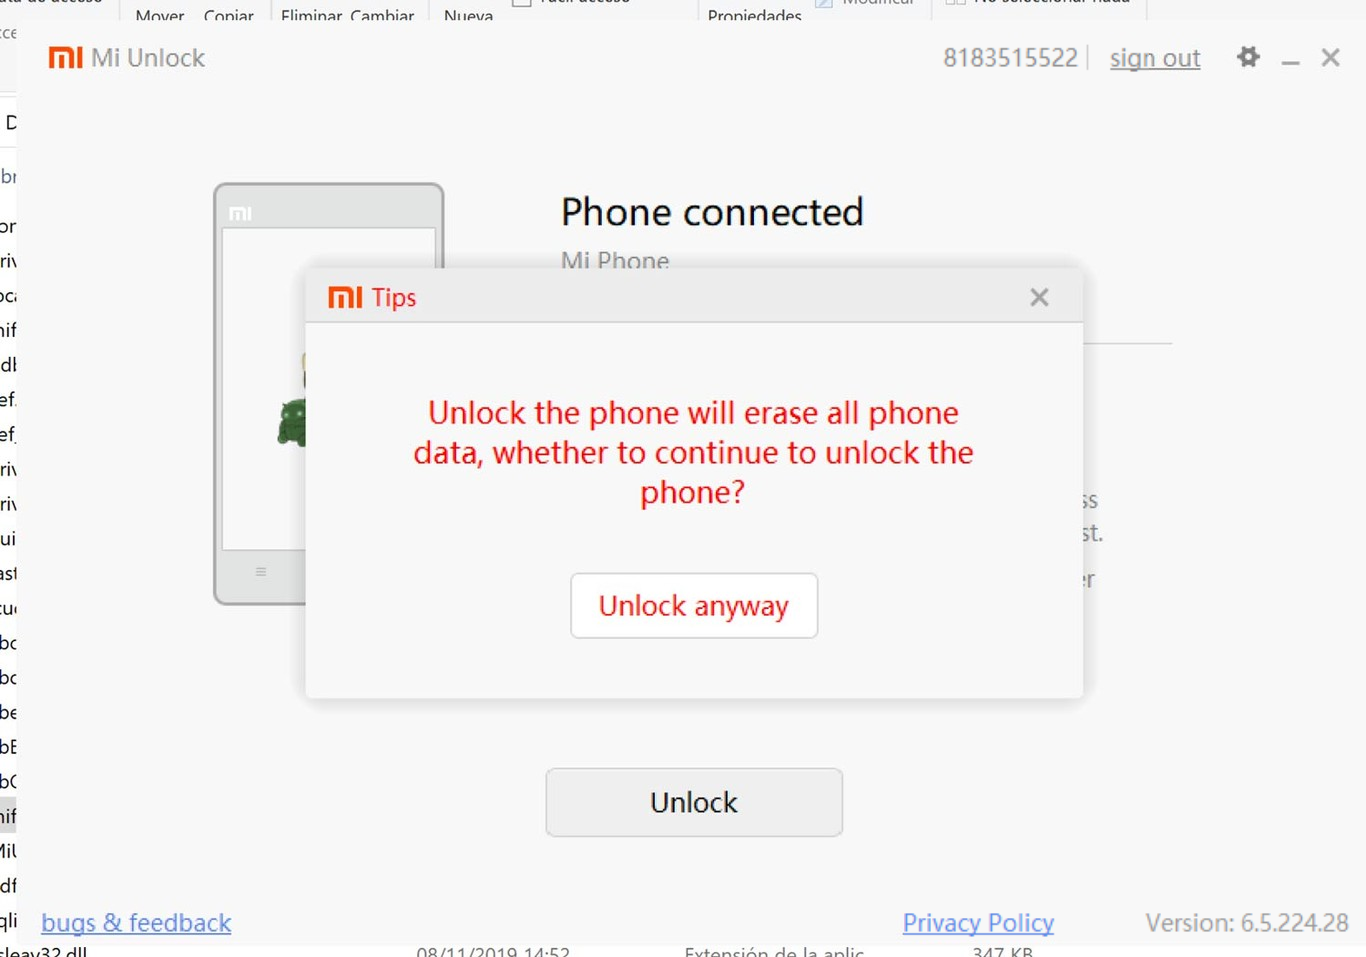
\includegraphics[width=0.8\textwidth]{figuras/root3.png}
  \caption[Pantalla de advertencia previa a desbloqueo de \textit{Mi Unlock}]{Pantalla de advertencia previa a desbloqueo de \textit{Mi Unlock}\\
  }
  \label{fig:root3}
\end{figure}

Tras aceptar, \textit{Mi Unlock} comprueba que tanto cuenta como dispositivo son aptos. Si eso es así, el programa envía una solicitud a los servidores de Xiaomi con el dispositivo asociado. Tras ello, en la pantalla del programa aparecerá el tiempo que se debe esperar hasta el desbloqueo del dispositivo (siete días).

\begin{figure}[H] 
\centering
  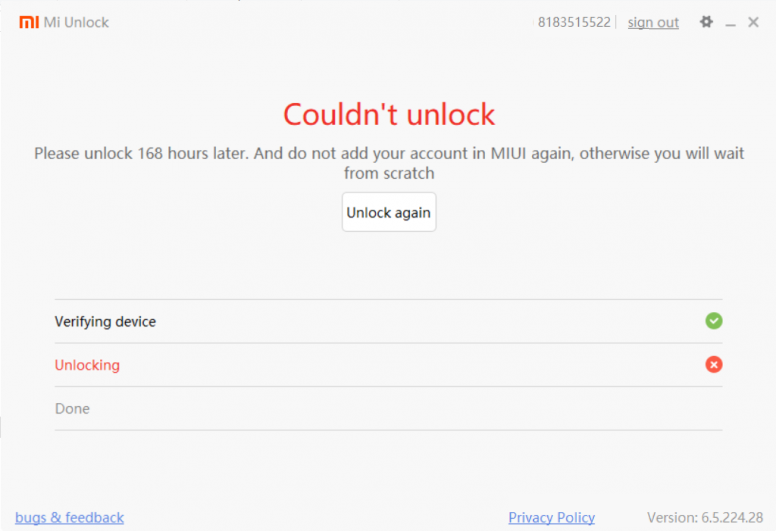
\includegraphics[width=0.7\textwidth]{figuras/root4.png}
  \caption[Pantalla de aviso de tiempo a esperar para desbloqueo de dispositivo mediante \textit{Mi Unlock}]{Pantalla de aviso de tiempo a esperar para desbloqueo de dispositivo mediante \textit{Mi Unlock}\\
  }
  \label{fig:root4}
\end{figure}

Tras transcurrir esa semana, se puede retomar el proceso de desbloqueo. Se repiten los mismos pasos con \textit{Mi Unlock} y se espera a que finalice el proceso. En el caso de que no se hubiera cumplido el tiempo de espera la aplicación informa de cuántas horas quedan para retomar este proceso. Antes de iniciar con el desbloqueo se deben hacer copias de seguridad dado que este proceso reestablece el dispositivo a los valores de fábrica.

\begin{figure}[H] 
\centering
  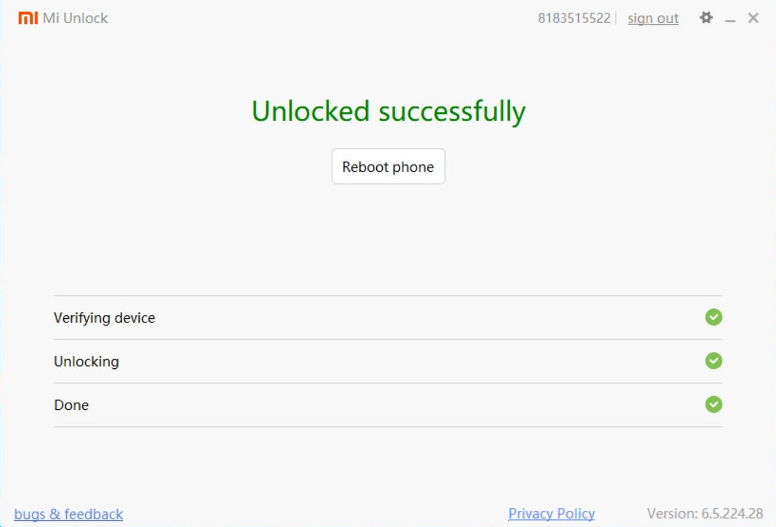
\includegraphics[width=0.7\textwidth]{figuras/root5.png}
  \caption[Pantalla de aviso de dispositivo correcto en \textit{Mi Unlock}]{Pantalla de aviso de dispositivo correcto en \textit{Mi Unlock}\\
  }
  \label{fig:root5}
\end{figure}

Se debe volver a iniciar el dispositivo en modo \textit{fastboot} para instalar el modo \textit{recovery} (recuperador del sistema operativo) \textit{TWRP} (\textit{Team Win Recovery Project}, un recovery personalizado para instalar ROM, restaurar copias de seguridad, rootear el dispositivo...) para poder continuar con la prueba.

Además, hay que instalar el \textit{Android Debug Bridge} (ADB), una herramienta de línea de comandos que permite realizar algunas acciones en el dispositivo, tales como instalar o depurar apps, y proporciona acceso a un shell para poder ejecutar distintos comandos en un smartphone.

Se vuelve a conectar el PC y se conecta el dispositivo a mediante un cable USB al PC con la depuración USB del mismo activada. En una ventana del símbolo del sistema, en la carpeta en la que se encuentran los drivers ADB se ejecuta el siguiente comando.

\textit{adb reboot bootloader}

Con ello se inicia el dispositivo en modo \textit{fastboot}.

Posteriormente, tras descargar la versión correspondiente de TWRP, se introducen los siguientes comandos desde el símbolo de sistema para actualizar al nuevo \textit{recovery TWRP}.

fastboot flash recovery twrp.img

fastboot boot twrp.img

Tras ello, el nuevo modo \textit{recovery} de este dispositivo será el de TWRP.

\begin{figure}[H] 
\centering
  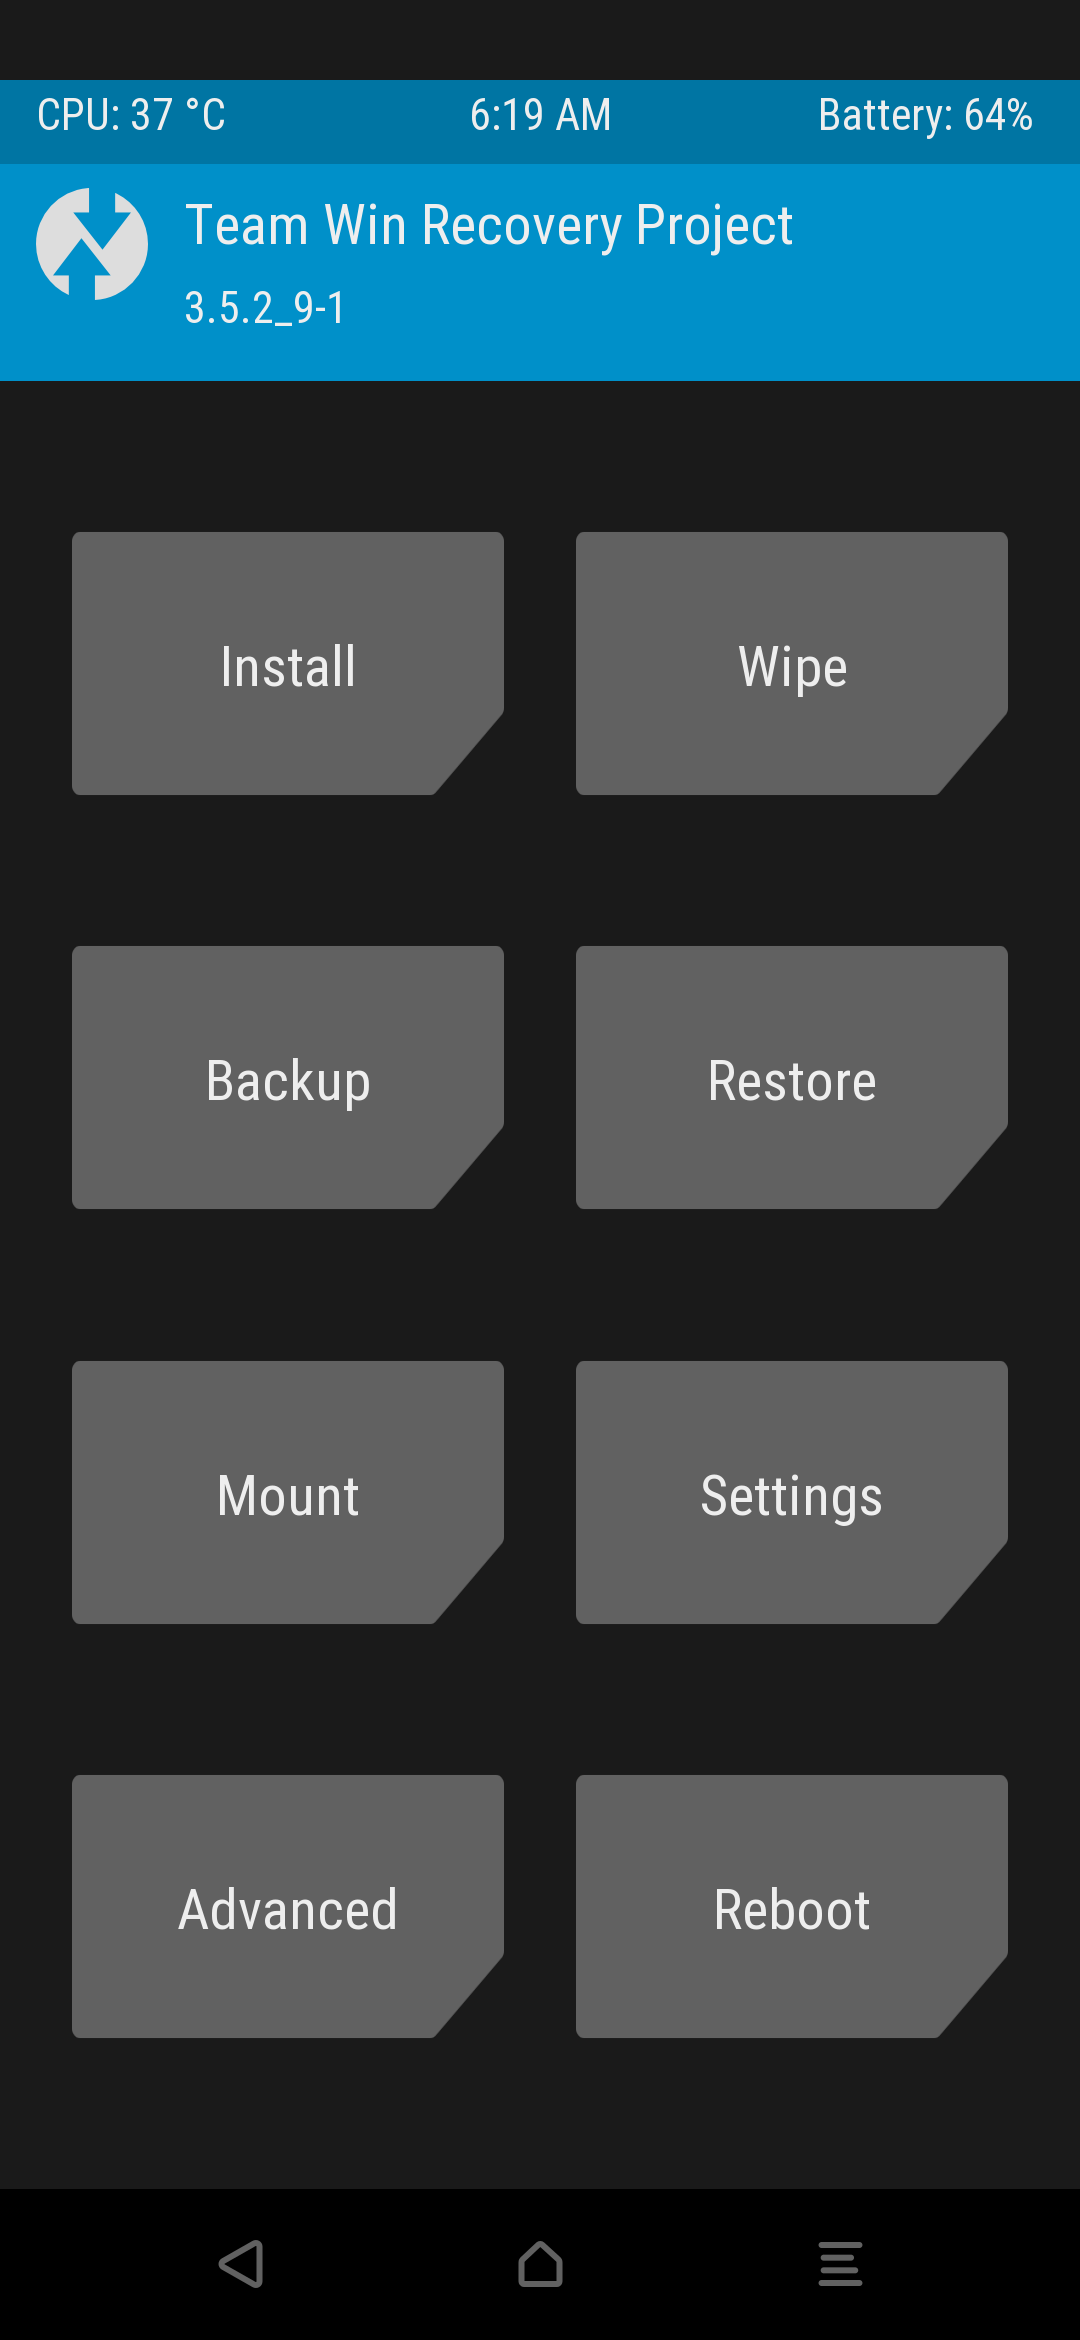
\includegraphics[width=0.4\textwidth]{figuras/root51.png}
  \caption[Pantalla principal de TWRP]{Pantalla principal de TWRP\\
  }
  \label{fig:root51}
\end{figure}


Ya desde \textit{TWRP} en primer lugar se formatea el equipo y se reinicia en modo \textit{recovery} después para que quede correctamente instalado.

\begin{figure}[H] 
\centering
  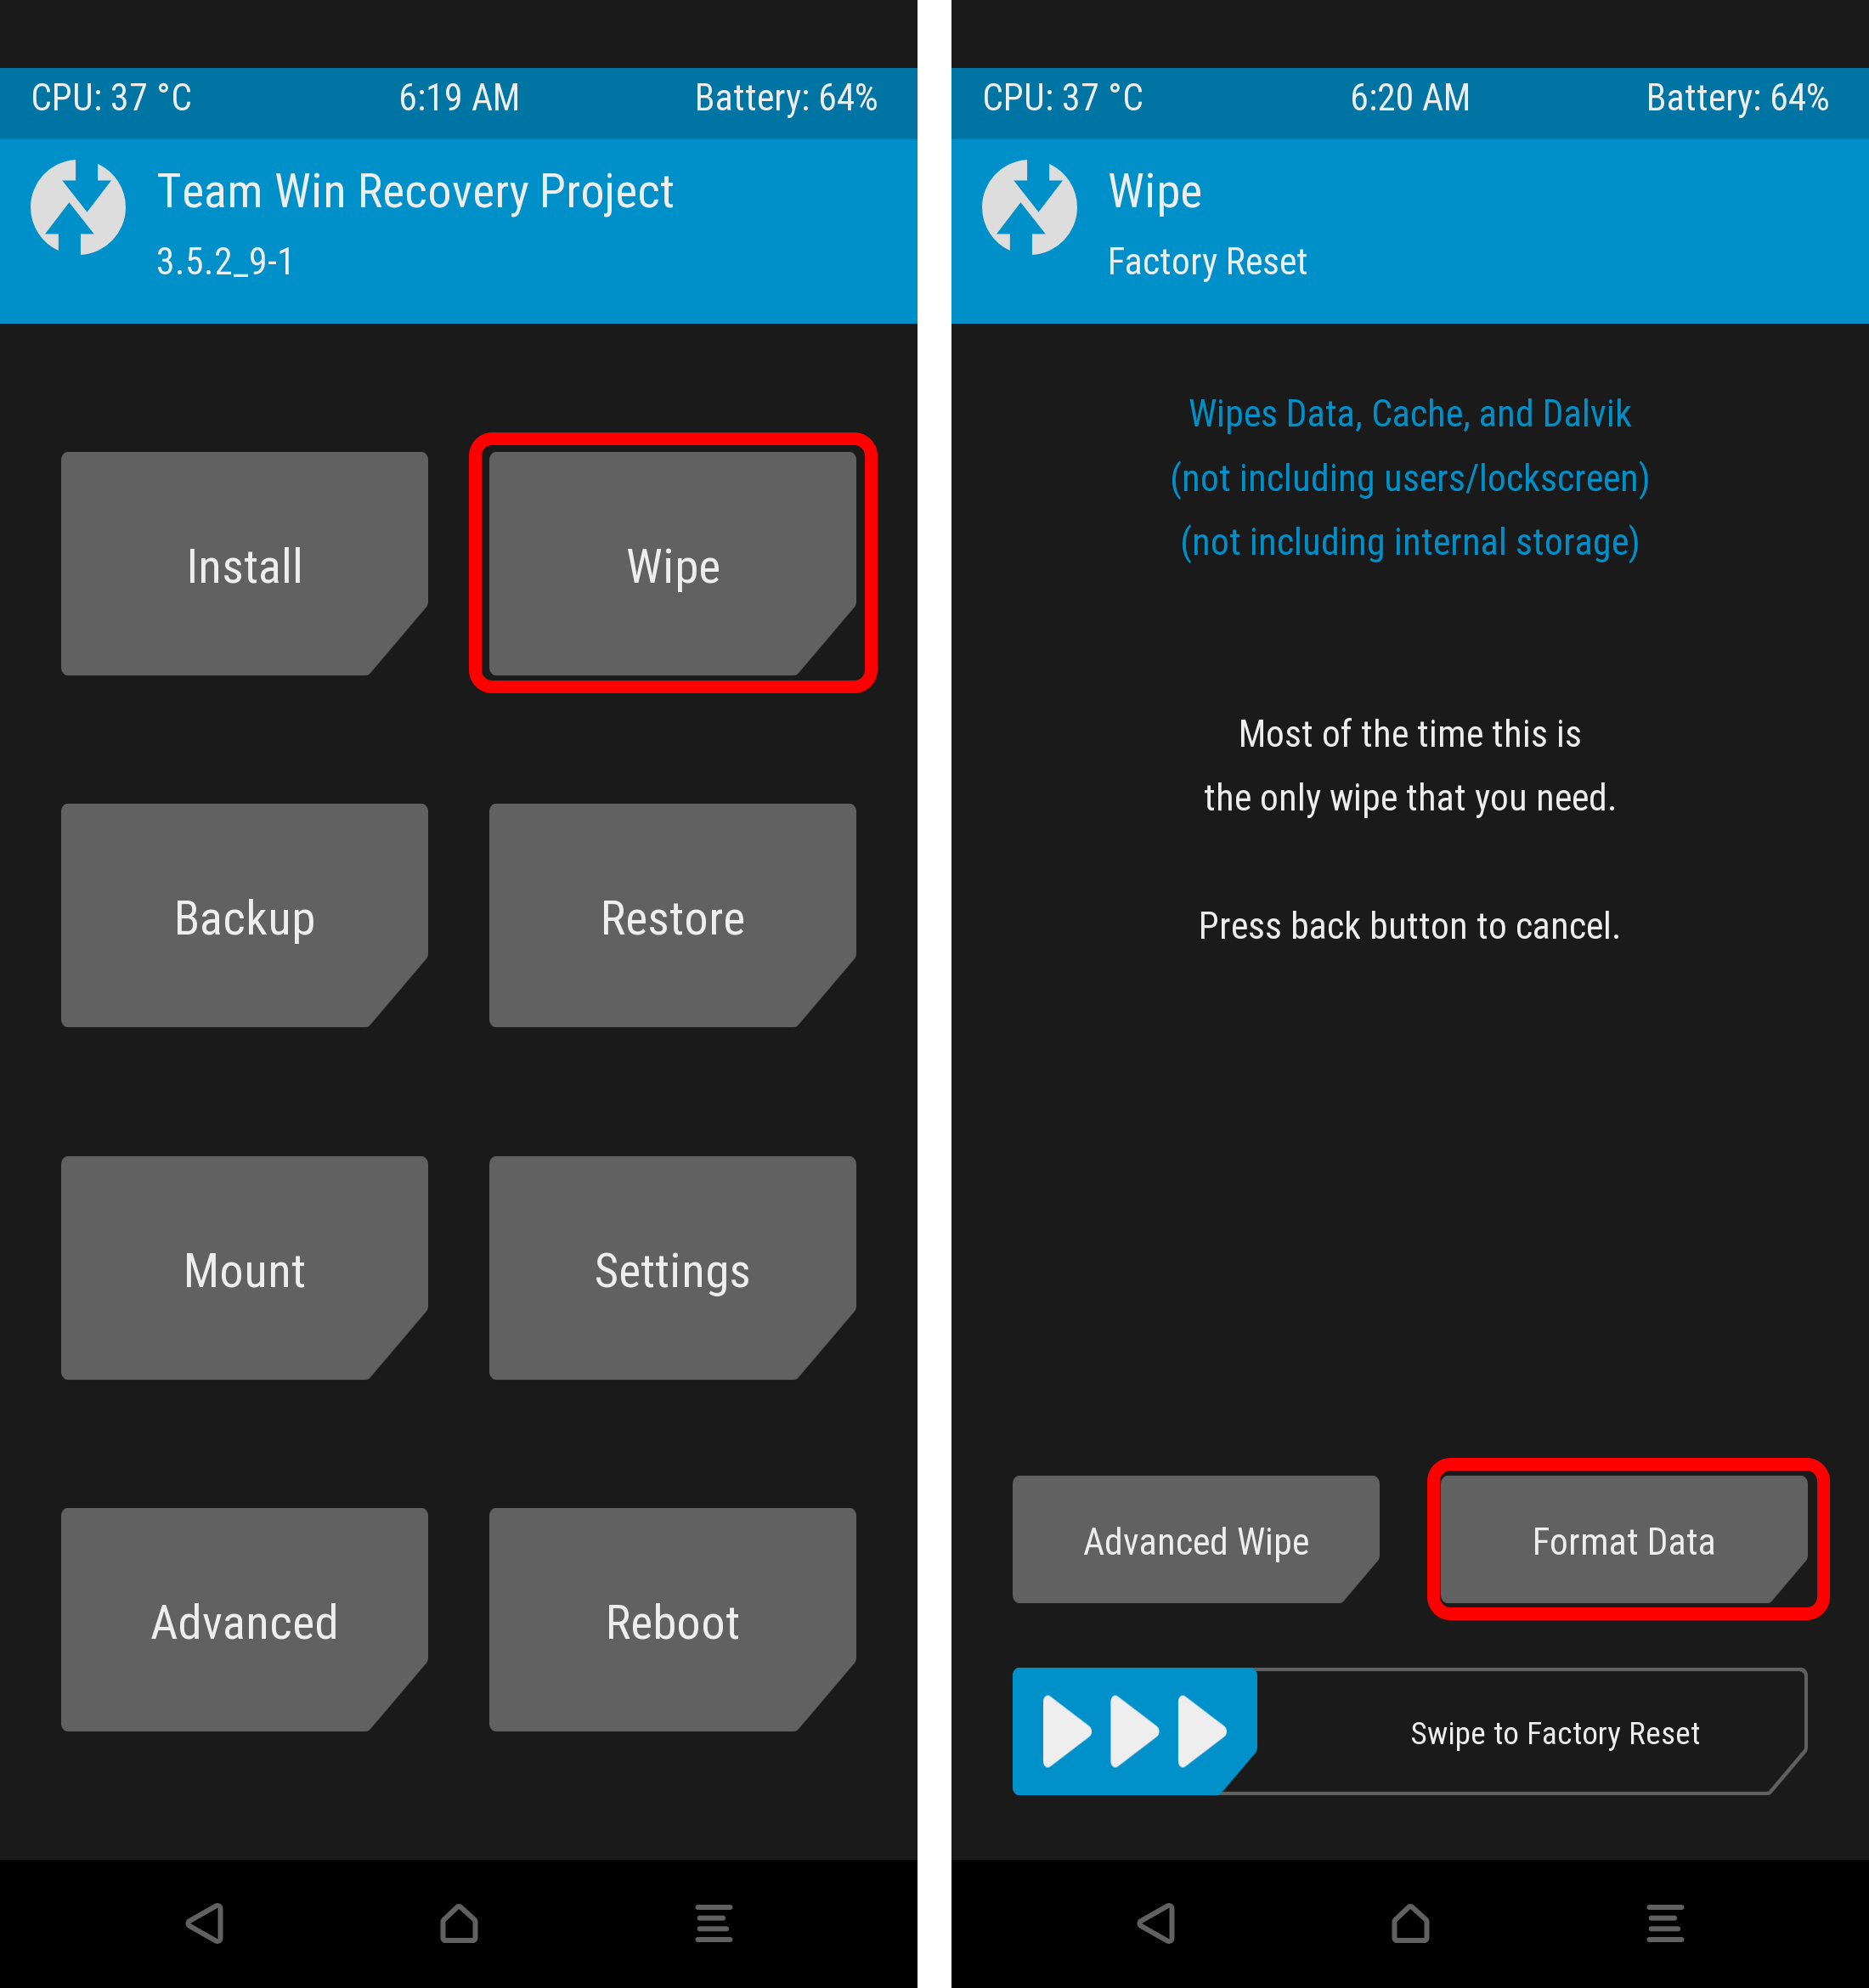
\includegraphics[width=0.4\textwidth]{figuras/root52.png}
  \caption[Proceso para formatear el dispositivo]{Proceso para formatear el dispositivo\\
  }
  \label{fig:root52}
\end{figure}

\begin{figure}[!h] 
\centering
  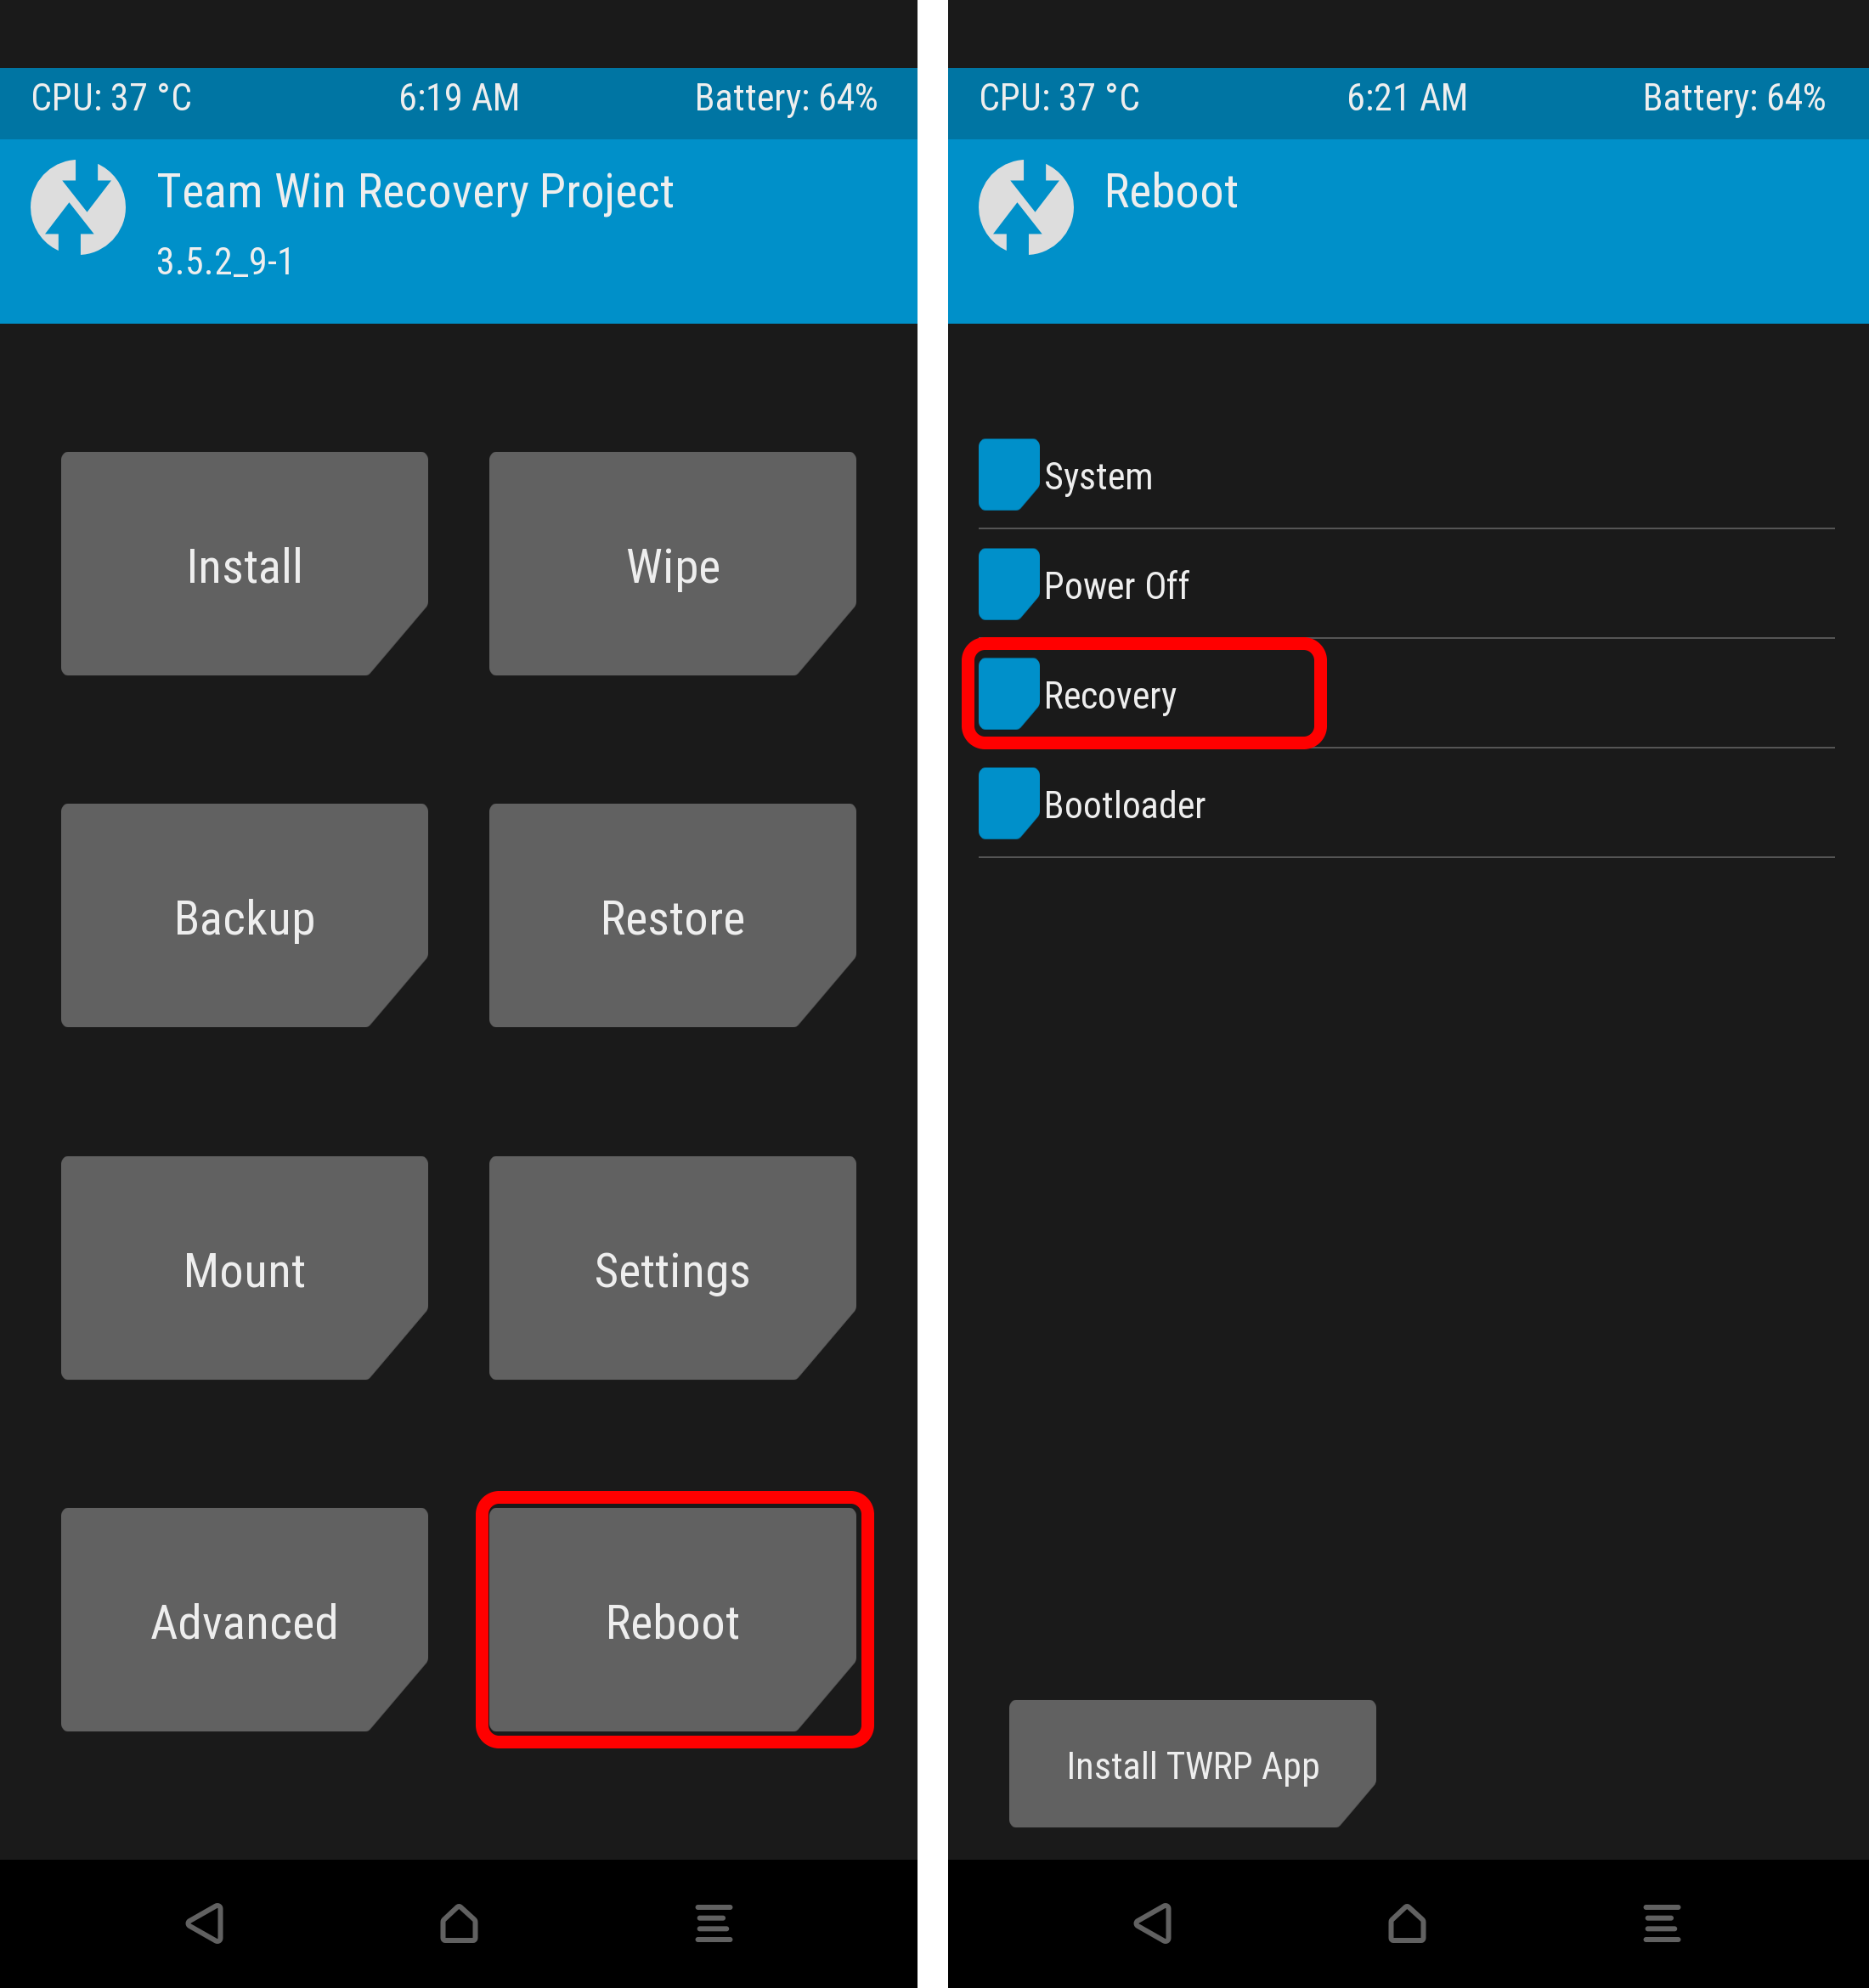
\includegraphics[width=0.4\textwidth]{figuras/root53.png}
  \caption[Proceso para reiniciar en modo recovery]{Proceso para reiniciar en modo recovery\\
  }
  \label{fig:root53}
\end{figure}


En último lugar, se deben descargar y copiar al dispositivo las versiones correctas, según el dispositivo que se utilice, en extensión ZIP de los ficheros de instalación de Magisk y Disable\_DM-Veritypor ese orden  para poder rootear el dispositivo.

\begin{figure}[H] 
\centering
  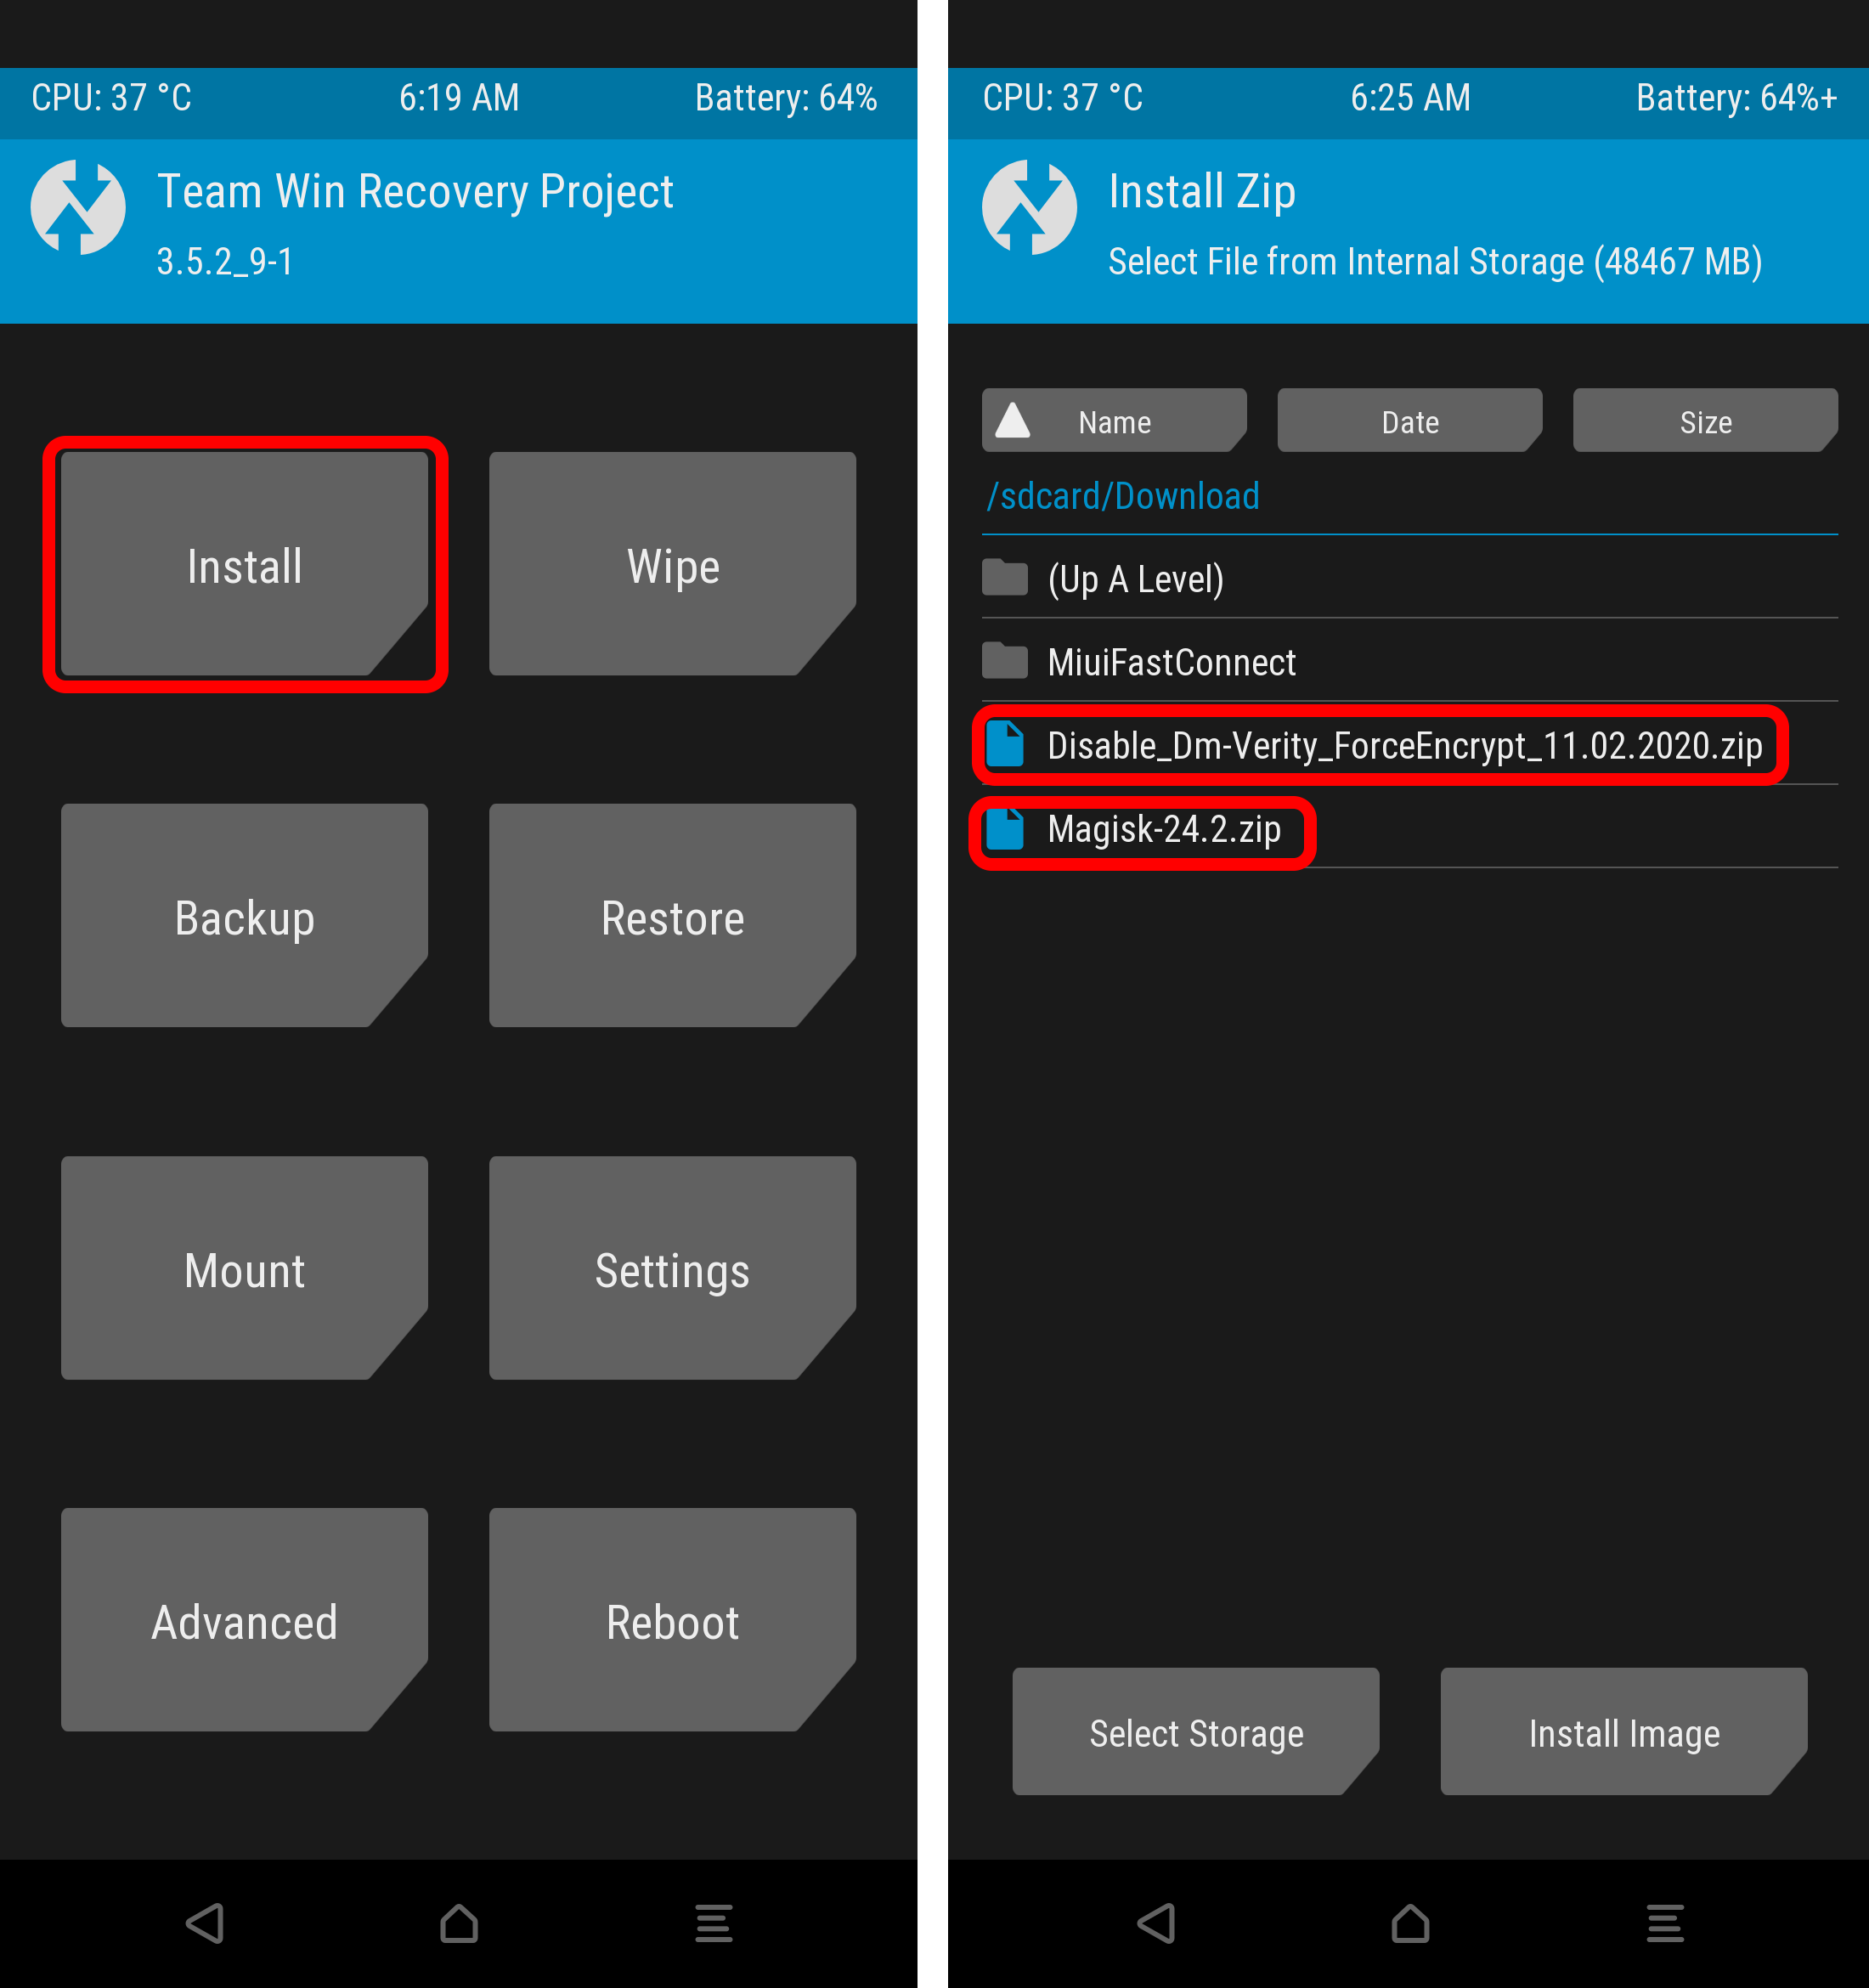
\includegraphics[width=0.4\textwidth]{figuras/root54.png}
  \caption[Proceso para instalar ficheros zip para rootear]{Proceso para instalar ficheros zip para rootear\\
  }
  \label{fig:root54}
\end{figure}

Con todo ello, el smartphone quedará rooteado y ya se puede pasar a realizar la prueba.

\begin{figure}[H] 
\centering
  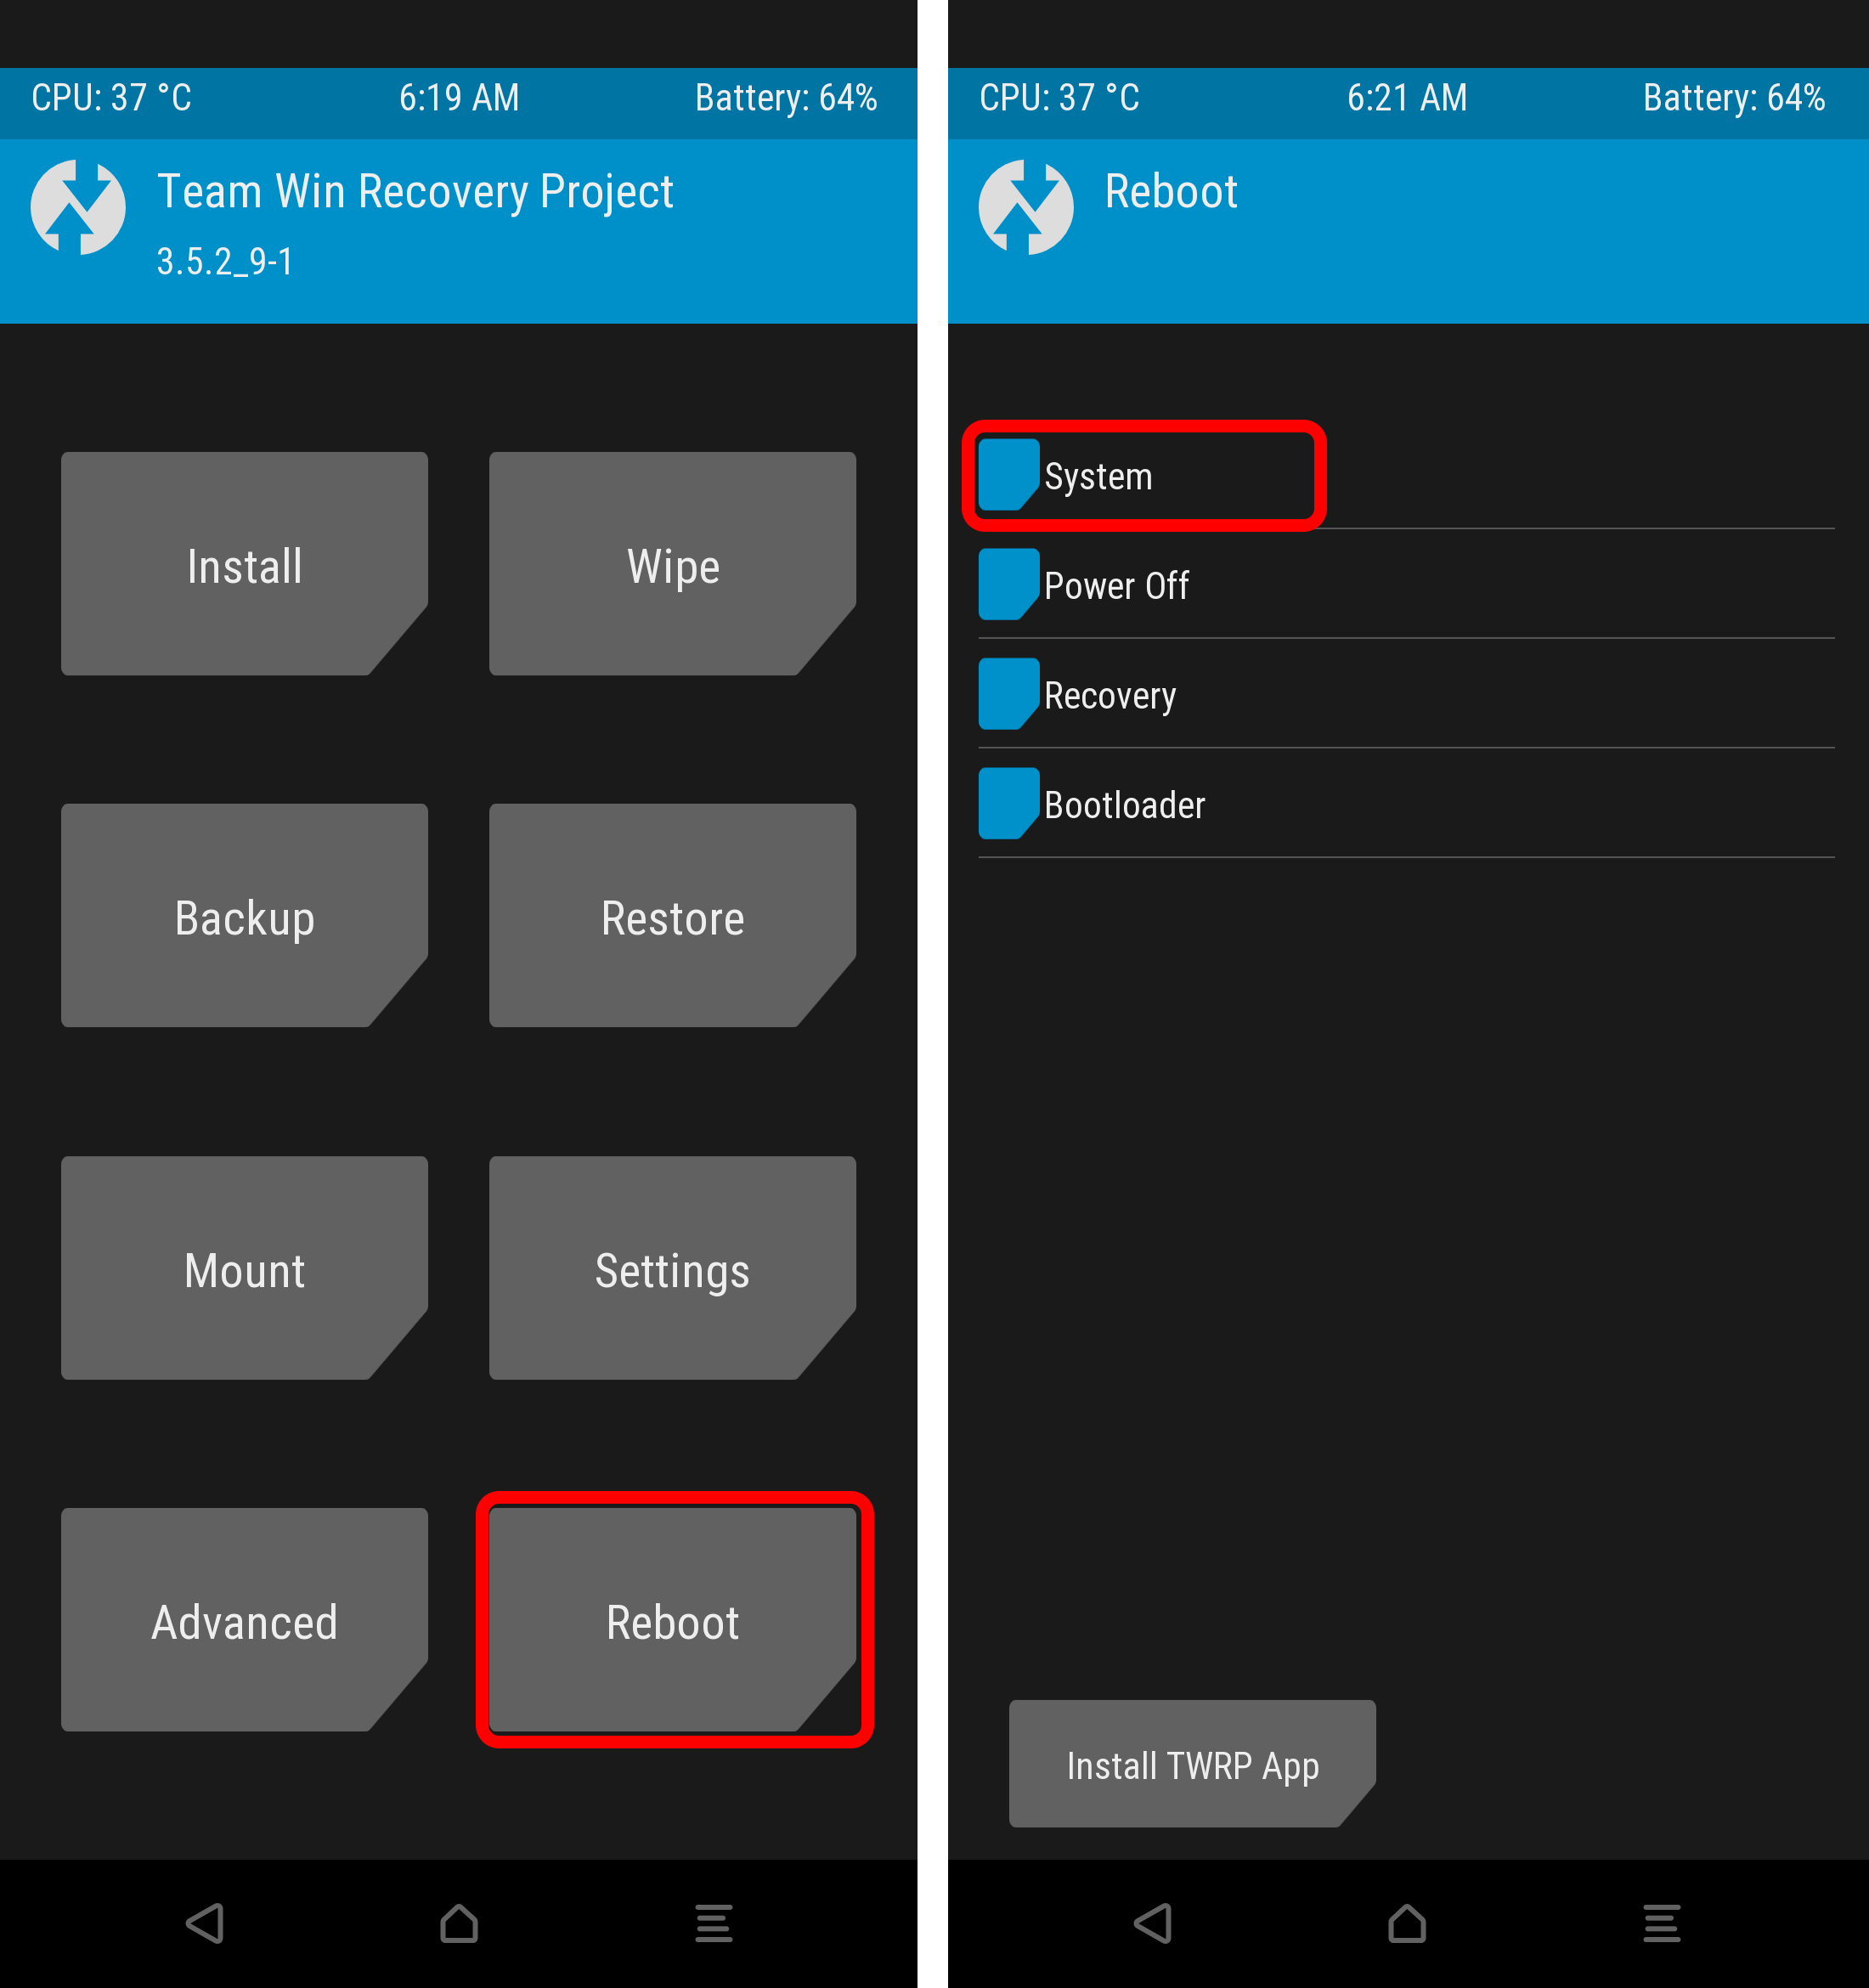
\includegraphics[width=0.4\textwidth]{figuras/root55.png}
  \caption[Proceso para iniciar el móvil en funcionamiento normal]{Proceso para iniciar el móvil en funcionamiento normal\\
  }
  \label{fig:root55}
\end{figure}

Para ello, se instala la aplicación llamada \textit{Emulador de tarjetas Pro (NFC Card Emulator Pro)}. 


\begin{figure}[H] 
\centering
  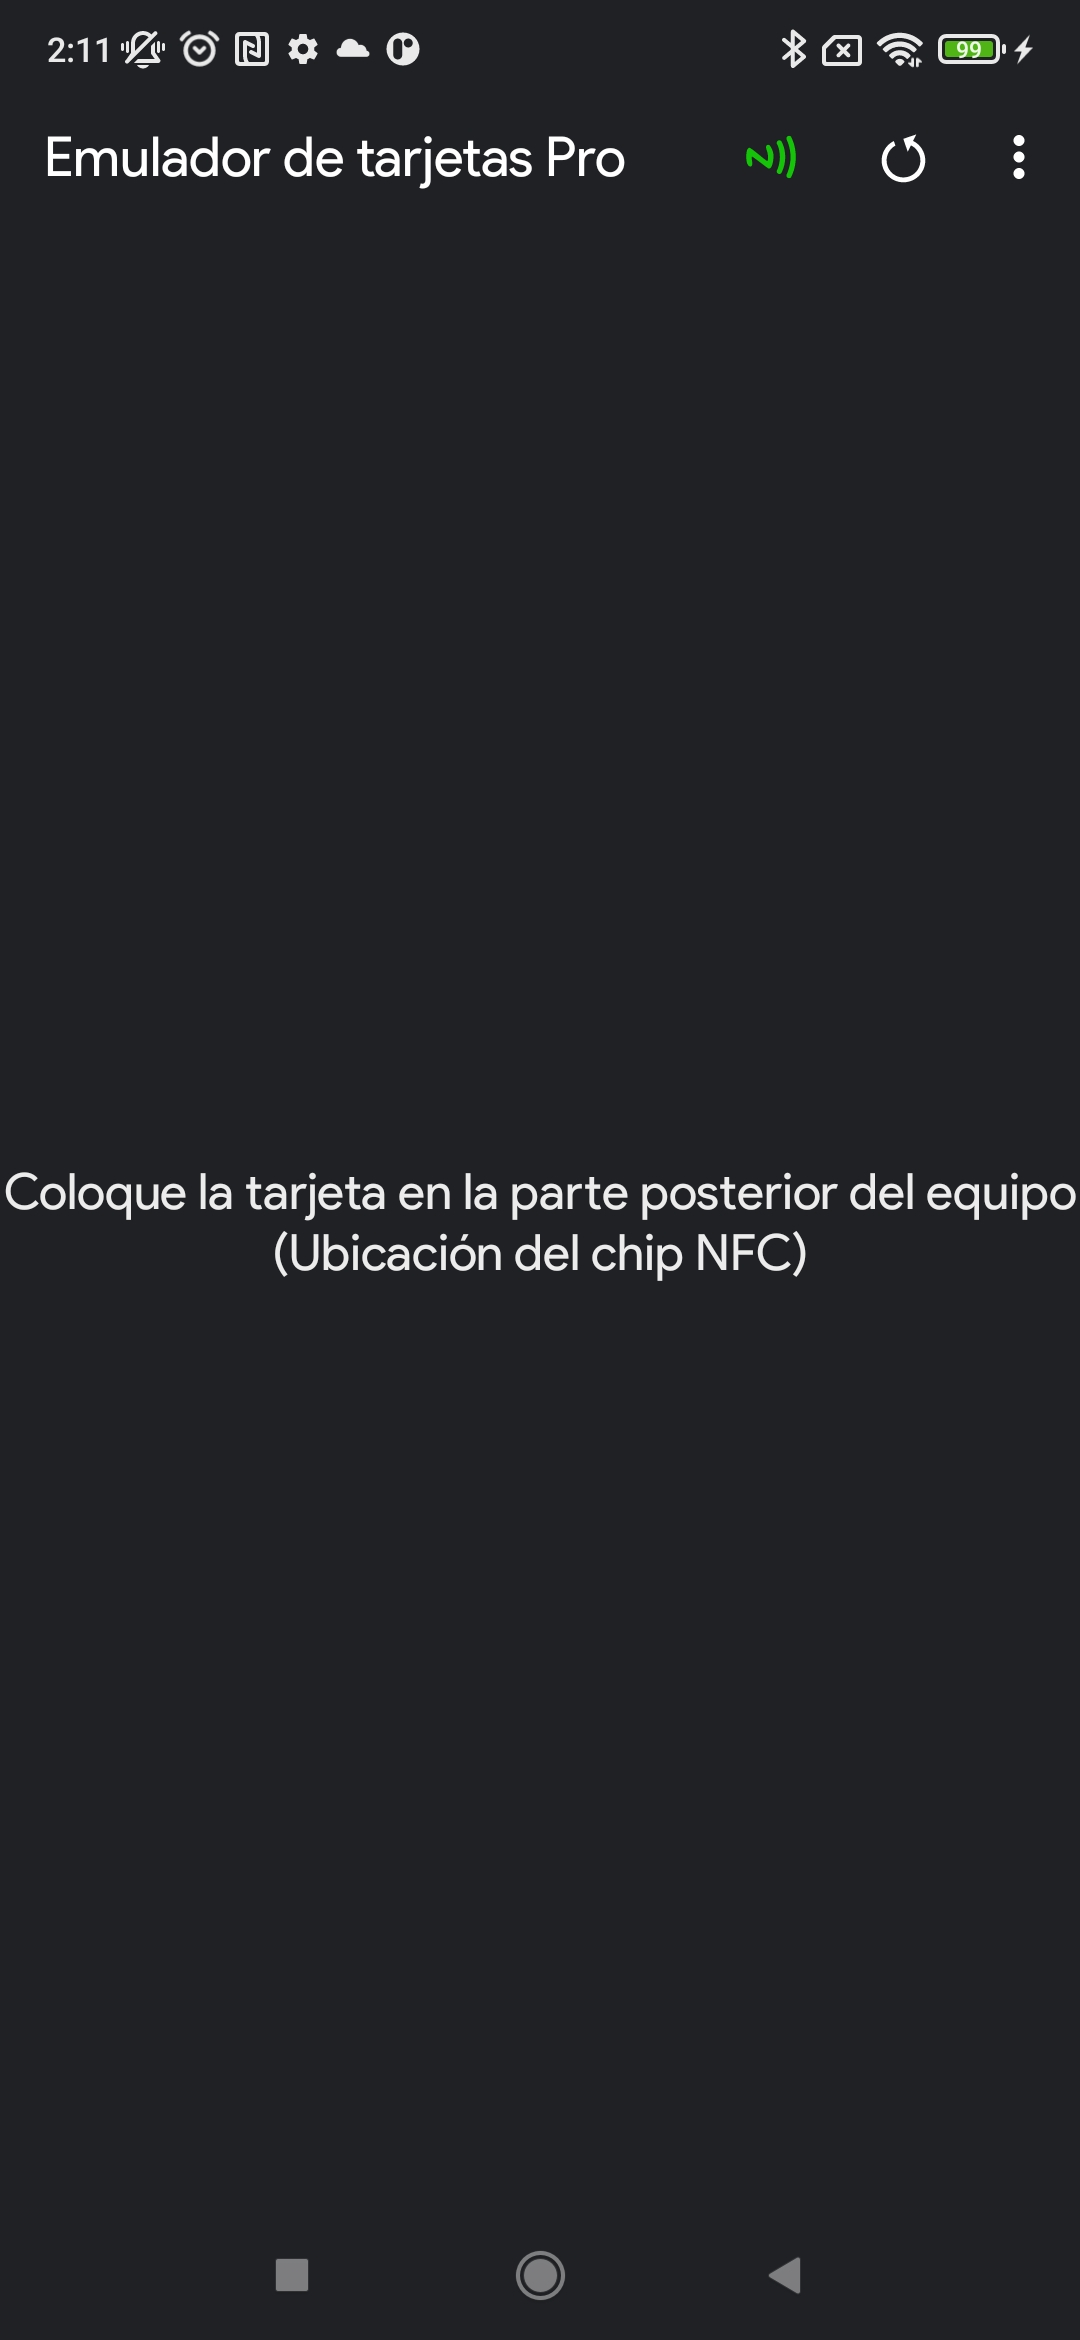
\includegraphics[width=0.4\textwidth]{figuras/root6.png}
  \caption[Pantalla de \textit{Emulador de tarjetas Pro} tras instalar la app]{Pantalla de \textit{Emulador de tarjetas Pro} tras instalar la app\\
  }
  \label{fig:root6}
\end{figure}

Desde la app se indica que se coloque la tarjeta en la parte posterior del equipo para leerla tras pulsar al primer botón de la parte superior izquierda de la pantalla. Se lee la tarjeta para disponer de la etiqueta de la misma y se guarda en \textit{Aceptar}.


\begin{figure}[H] 
\centering
  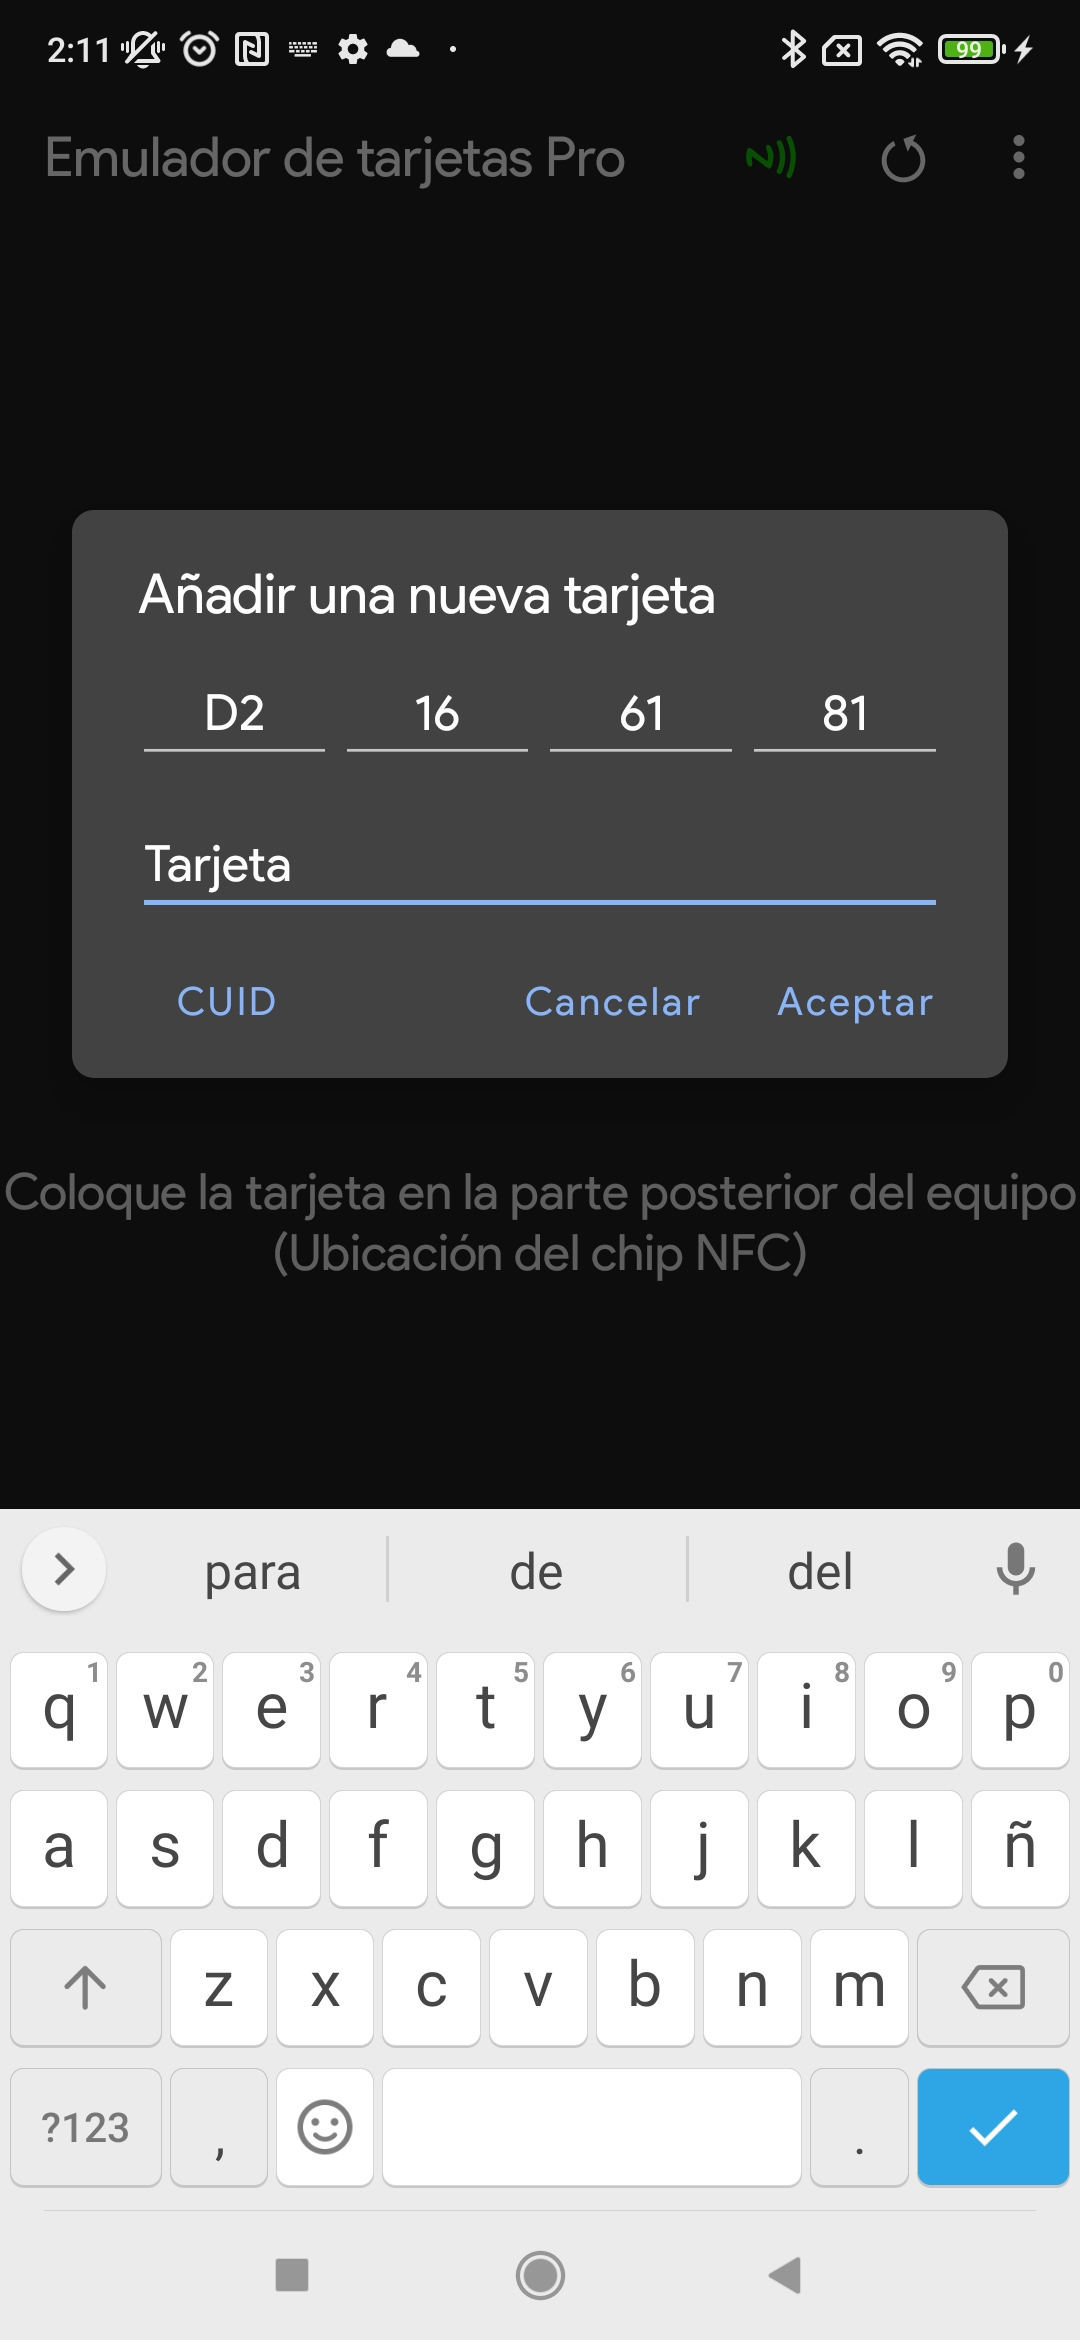
\includegraphics[width=0.4\textwidth]{figuras/root7.png}
  \caption[Pantalla de \textit{Emulador de tarjetas Pro} tras leer una tarjeta]{Pantalla de \textit{Emulador de tarjetas Pro} tras leer una tarjeta\\
  }
  \label{fig:root7}
\end{figure}

Se pulsa en el icono inferior derecho del interior de la tarjeta para emularla. Se acepta la solicitud de cualquier tipo de permiso. Con ello la tarjeta se emulará durante un tiempo en intervalos temporales cortos pero alternos, por lo que en varios momentos la tarjeta queda correctamente \textit{copiada} para simular el número de etiqueta de la tarjeta.


\begin{figure}[H] 
\centering
  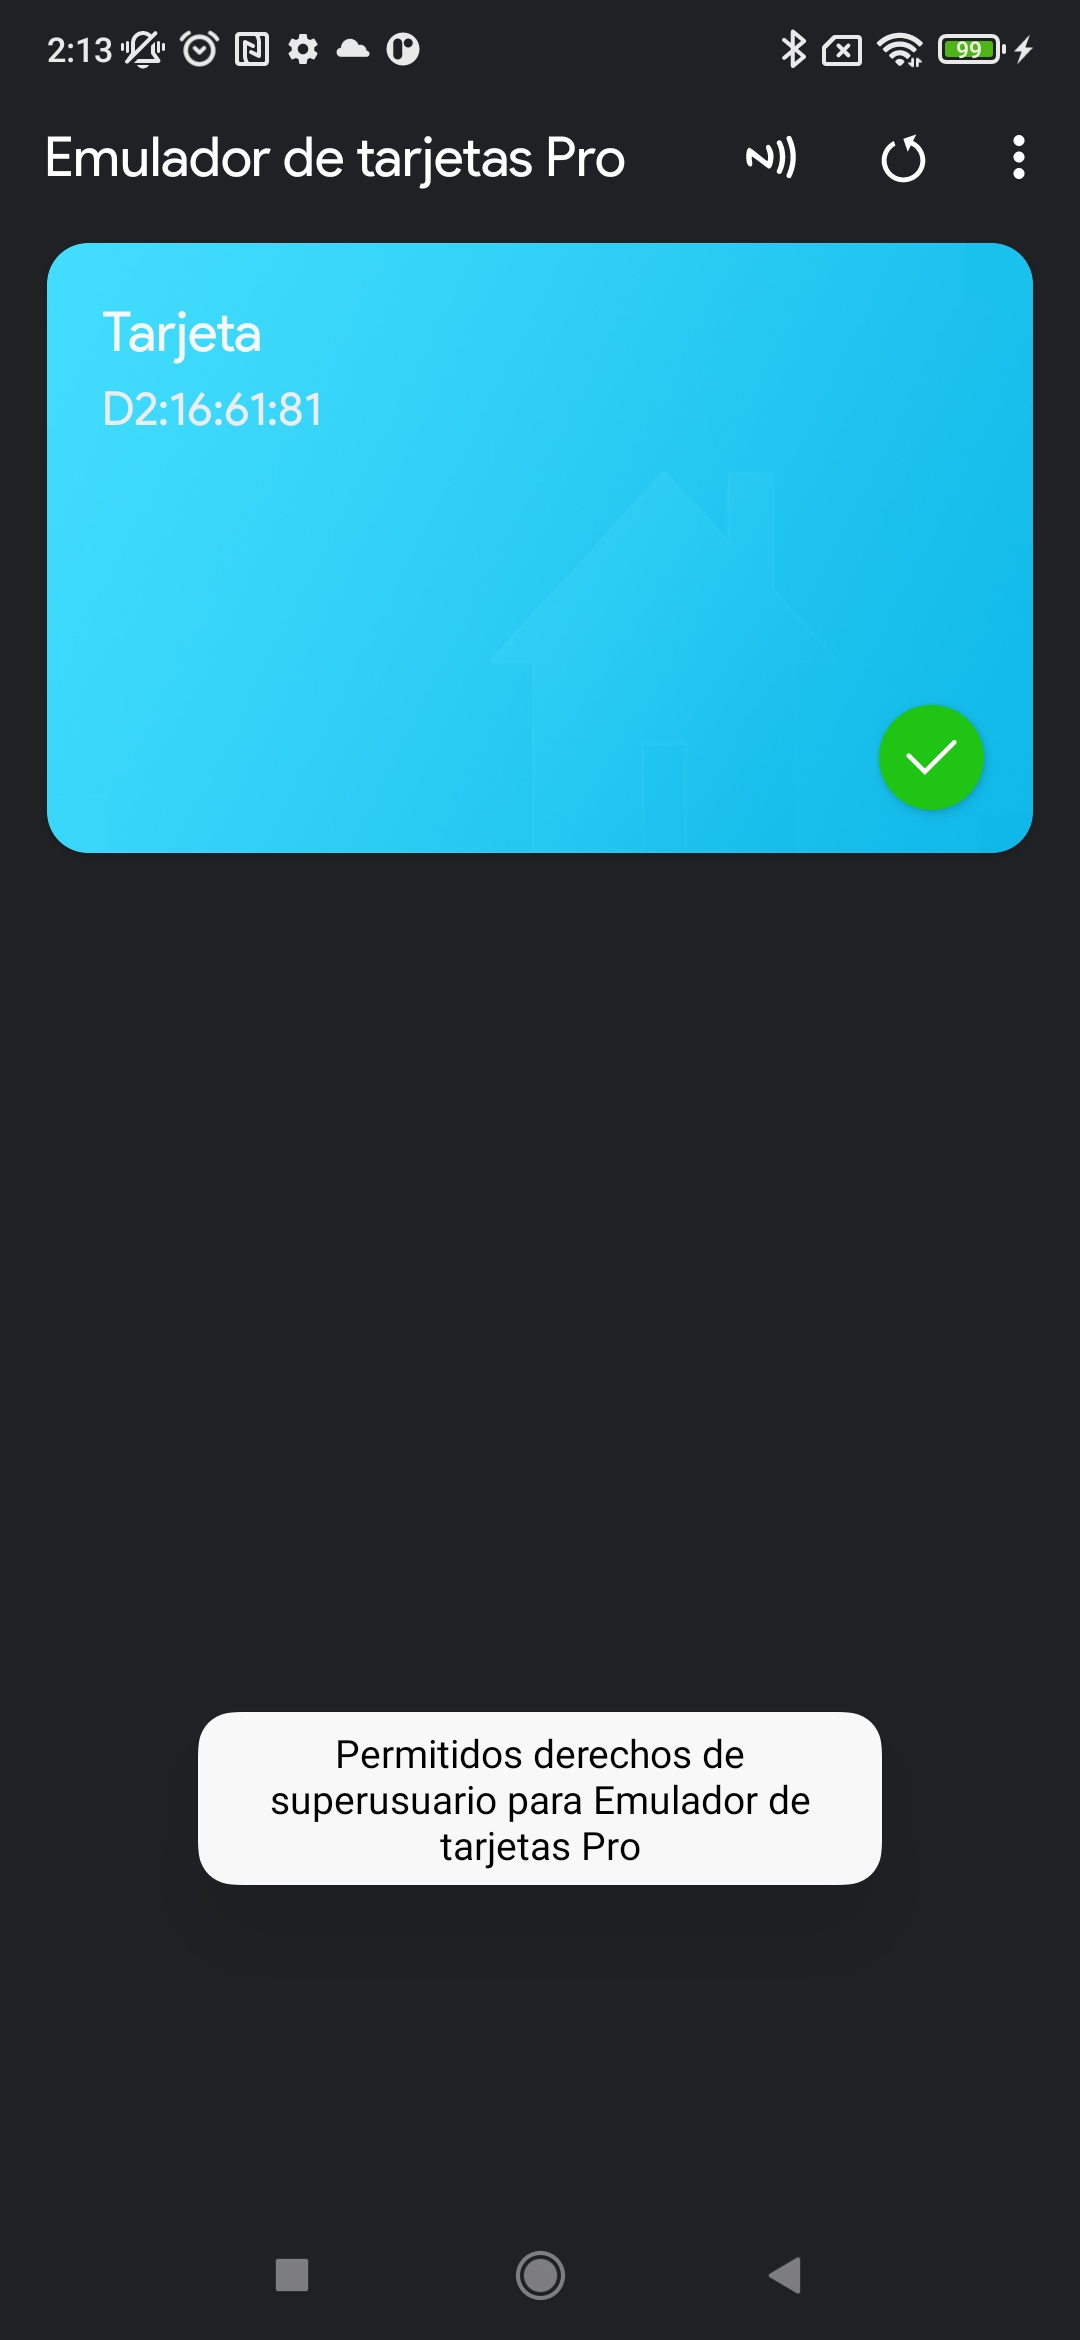
\includegraphics[width=0.4\textwidth]{figuras/root8.png}
  \caption[Pantalla de \textit{Emulador de tarjetas Pro} durante la emulación de una tarjeta]{Pantalla de \textit{Emulador de tarjetas Pro} durante la emulación de una tarjeta\\
  }
  \label{fig:root8}
\end{figure}

Para comprobar que esto funciona correctamente, se realiza una prueba pasando la tarjeta sobre el cargador, el cuál envía al servidor WebSocket un paquete de tipo \textit{Authorize}. Las operaciones del cargador utilizado (\textit{Alfen EVe mini}) se pueden revisar con el programa \textit{Ace Service Installer} siempre y cuando este se encuentre en la misma red que el ordenador desde el que se accede a este programa.


\begin{figure}[H] 
\centering
  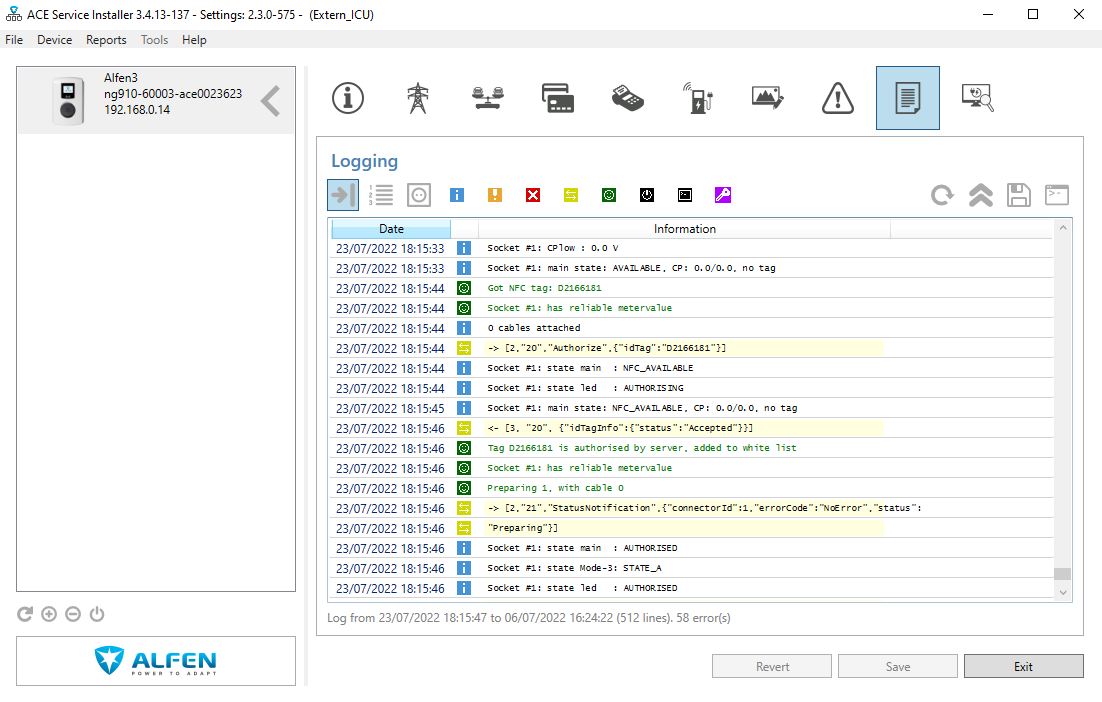
\includegraphics[width=1\textwidth]{figuras/authorize1.png}
  \caption[Pantalla de logs de \textit{Ace Service Installer} tras el paso de tarjeta]{Pantalla de logs de \textit{Ace Service Installer} tras el paso de tarjeta\\
  }
  \label{fig:authorize1}
\end{figure}

Ahora, durante la emulación de la tarjeta, se pasa el smartphone por encima del punto de recarga para ver si el paso se produce correctamente. Se ve que, efectivamente, es así.


\begin{figure}[H]
\centering
  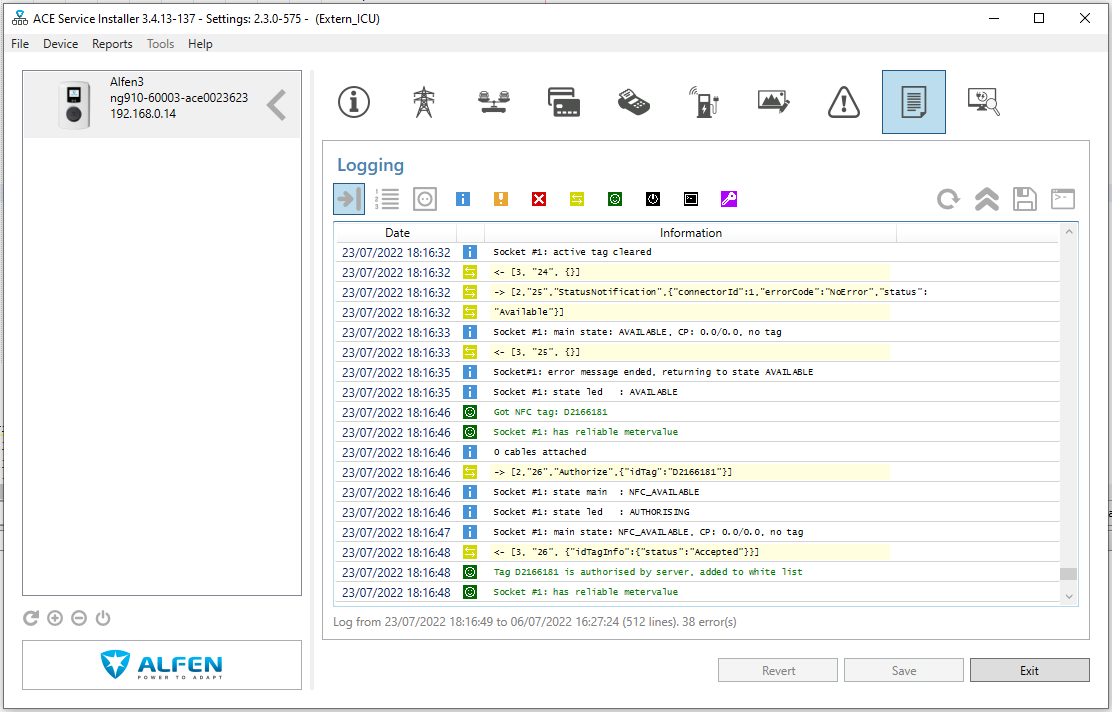
\includegraphics[width=1\textwidth]{figuras/authorize2.png}
  \caption[Pantalla de logs de \textit{Ace Service Installer} tras el paso del smartphone que simula la tarjeta]{Pantalla de logs de \textit{Ace Service Installer} tras el paso del smartphone que simula la tarjeta\\
  }
  \label{fig:authorize2}
\end{figure}


Un caso similar a este se puede ver en el siguiente ejemplo de la página de \textit{eventos de los cargadores} de la web.

\begin{figure}[H] 
\centering
  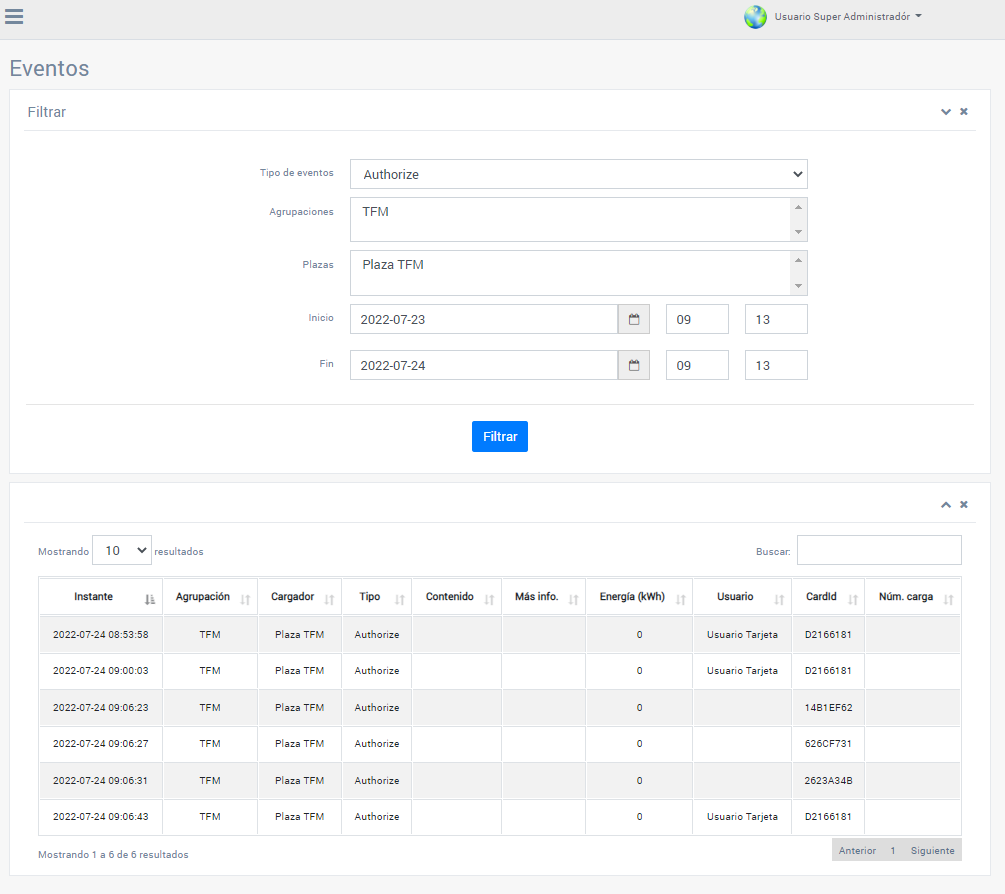
\includegraphics[width=1\textwidth]{figuras/authorize3.png}
  \caption[Pantalla de eventos de la web tras los pasos de las etiquetas]{Pantalla de eventos de la web tras los pasos de las etiquetas\\
  }
  \label{fig:authorize3}
\end{figure}



\subsubsection{Configuración previa a las soluciones}
Mediante un software del fabricante (\textit{Ace Service Installer}) que se puede comunicar con el punto de recarga se realiza una configuración previa en base a lo tratado antes en \ref{OCPP}:

\begin{figure}[H] 
\centering
  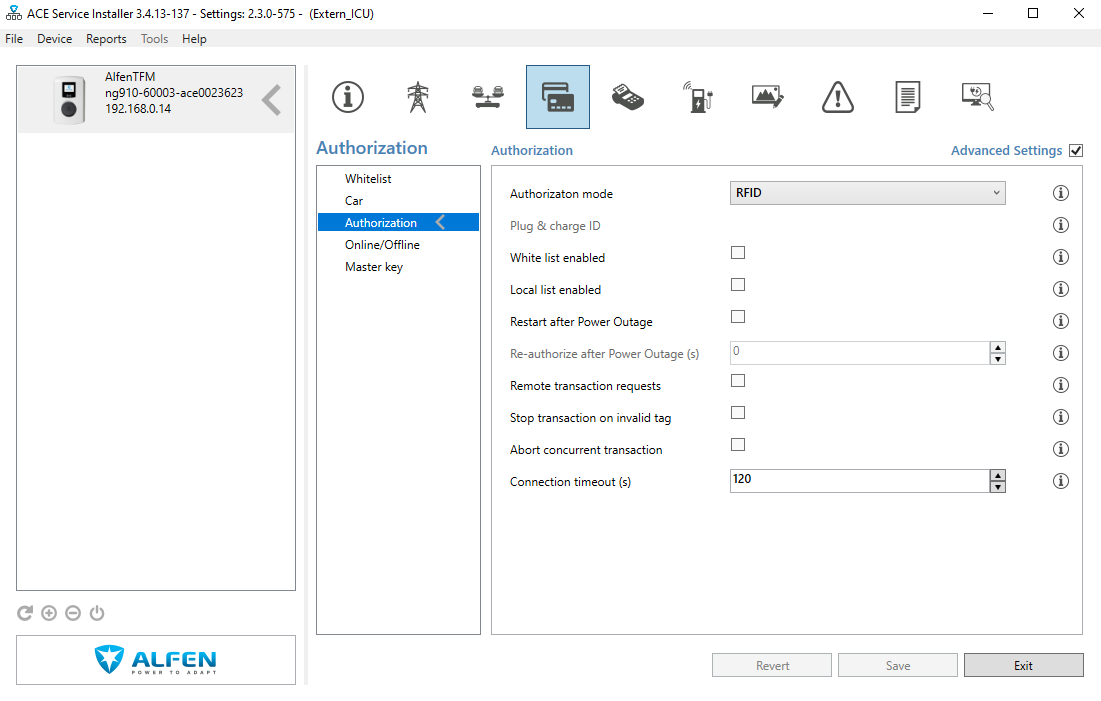
\includegraphics[width=1\textwidth]{figuras/conf1.png}
  \caption[Pantalla de configuración de autorización general del punto de recarga]{Pantalla de configuración de autorización general del punto de recarga\\
  }
  \label{fig:conf1}
\end{figure}

En primer lugar se desactivan las \textit{White list} y la \textit{Local list} para evitar que estas puedan generar algún tipo de caché que guarde las etiquetas. Se evita también que las recargas se paren con un número de etiqueta erróneo.


\begin{figure}[H] 
\centering
  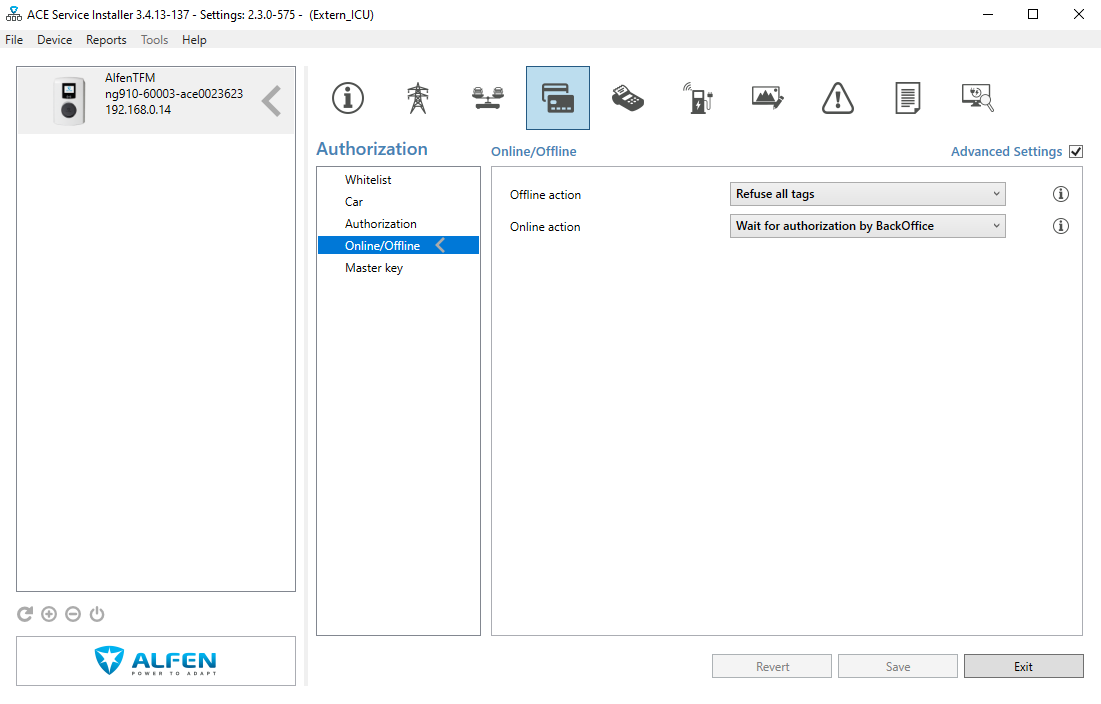
\includegraphics[width=1\textwidth]{figuras/conf2.png}
  \caption[Pantalla de configuración de autorización según conexión del punto de recarfa]{Pantalla de configuración de autorización según conexión del punto de recarga\\
}
  \label{fig:conf2}
\end{figure}

Se configuran las actuaciones online y offline. En offline (si el punto tiene algún problema de conexión) no se autoriza nada y en modo conectado siempre tiene que esperar por la respuesta del CSMS.


\begin{figure}[H] 
\centering
  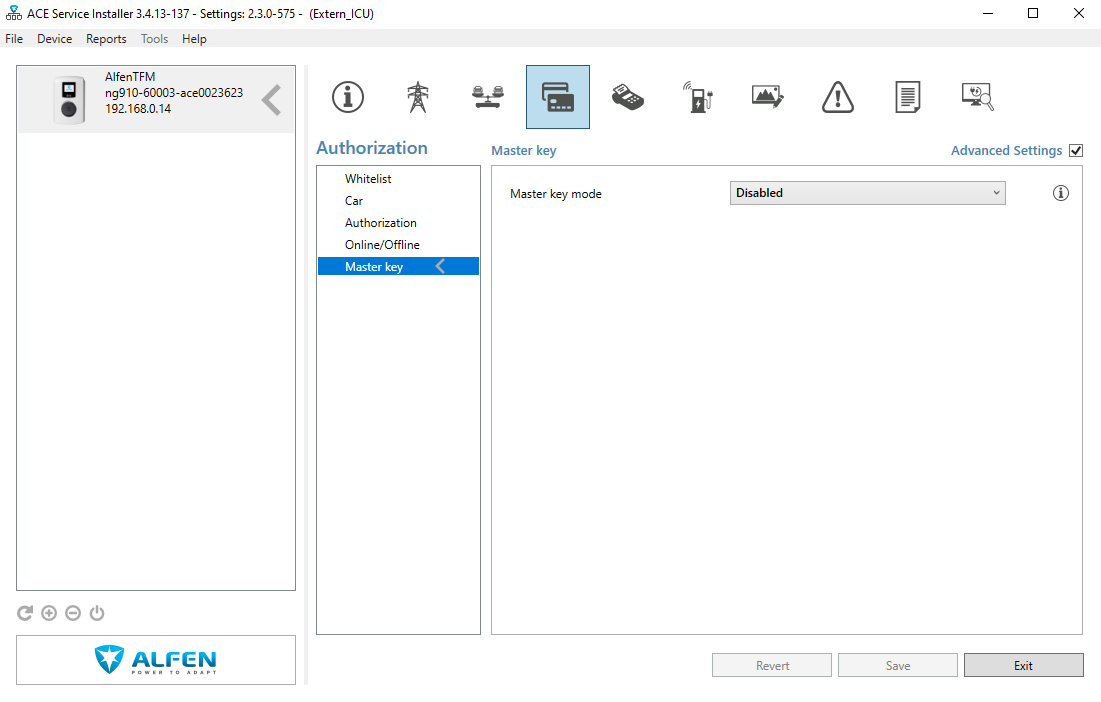
\includegraphics[width=1\textwidth]{figuras/conf3.png}
  \caption[Pantalla de configuración de autorización con clave maestra del punto de recarga]{Pantalla de configuración de autorización con clave maestra  del punto de recarga\\
}
  \label{fig:conf3}
\end{figure}

Se desactiva asimismo la posibilidad de funcionar con una clave maestra.

Con todo ello configurado ya se podrían realizar de forma correcta las pruebas de las soluciones propuestas en este proyecto.



\subsubsection{Posibles soluciones}

Como se trató anteriormente existen tres soluciones cuyas pruebas se diseminan en este apartado. Las dos primeras basadas una en una autenticación 2FA y en NFC con etiqueta variable respectivamente y la tercera de ellas es la combinación de ambas. 

\subsubsubsection{Autenticación 2FA}

En esta prueba se simularán un inicio tanto con un paso de tarjeta en el EVSE como una petición desde el servicio web.

\begin{figure}[H] 
\centering
  \includegraphics[width=0.5\textwidth]{figuras/prueba1.png}
  \caption[Pantalla del cargador en estado \textit{Libre}]{Pantalla del cargador en estado Libre\\
  }
  \label{fig:prueba1}
\end{figure}

En el primero de los casos el cargador sí que cambia de estado, con una pantalla de espera.

\begin{figure}[H] 
\centering
  \includegraphics[width=0.5\textwidth]{figuras/prueba2.png}
  \caption[Pantalla del cargador tras enviar un \textit{Authorize}]{Pantalla del cargador tras enviar un Authorize\\
  }
  \label{fig:prueba2}
\end{figure}

En el segundo, no hay ninguna modificación. A partir de aquí, el proceso es similar, llegando inmediatamente después de enviar la orden un correo electrónico con el código a introducir en la app.


\begin{figure}[H] 
\centering
  \includegraphics[width=0.5\textwidth]{figuras/prueba3.png}
  \caption[Ejemplo de correo electrónico que llega al usuario al solicitar un inicio de recarga]{Ejemplo de correo electrónico que llega al usuario al solicitar un inicio de recarga\\
  }
  \label{fig:prueba3}
\end{figure}

Tras introducirlo, se envía una orden de recarga al cargador y este inicia la recarga.

\begin{figure}[H] 
\centering
  \includegraphics[width=0.5\textwidth]{figuras/prueba4.png}
  \caption[Pantalla del EVSE mientras se realiza una recarga]{Pantalla del EVSE mientras se realiza una recarga\\
  }
  \label{fig:prueba4}
\end{figure}

La comprobación más importante, que es el que el cargador vuelva a su estado original en caso de un paso de tarjeta si no se realiza la segunda autorización, funciona correctamente. En caso de que un usuario robase la etiqueta de tarjeta no dispondría de acceso al usuario en la plataforma de la persona que es la legítima propietaria de la misma.

Al añadir ese punto intermedio del código de confirmación, por mucho que se disponga de los datos de etiqueta del usuario autorizado si no se dispone de los datos de acceso a la plataforma de la persona autorizada no se podrá iniciar la recarga.

\subsubsubsection{NFC variable}

En este caso lo interesante a probar es el paso de tarjeta mientras se realiza una recarga.

\begin{figure}[H] 
\centering
  \includegraphics[width=0.5\textwidth]{figuras/prueba5.png}
  \caption[Pantalla del EVSE al pasar una tarjeta mientras se realiza una recarga]{Pantalla del EVSE al pasar una tarjeta mientras se realiza una recarga\\
  }
  \label{fig:prueba5}
\end{figure}

Si se pasa la misma tarjeta que inició la recarga esta no se debería detener dado que además de esta tarjeta variable se ha creado una \textit{ficticia} en el inicio de recarga (se debe recordar que el propio cargador detiene una recarga iniciada con la misma etiqueta que se pase por el cargador al estar transcurriendo una recarga). Esto protege el sistema del robo de la etiqueta de la tarjeta al inicio de la sesión e impide que un usuario no autorizado pueda detener de algún modo la recarga del usuario que está cargando en ese momento. 

\begin{figure}[H] 
\centering
  \includegraphics[width=0.5\textwidth]{figuras/prueba6.png}
  \caption[Pantalla del EVSE al pasar una tarjeta mientras se realiza una recarga]{Pantalla del EVSE al pasar una tarjeta mientras se realiza una recarga\\
  }
  \label{fig:prueba6}
\end{figure}

En este caso hay que tratar de evitar que, aún robando el usuario la etiqueta con la que se inicia la recarga, esta no se pueda detener. Por ello, en primer lugar, aunque se pase una tarjeta, la etiqueta asociada a la recarga tiene que ser un número aleatorio. Esto es debido a que el cargador de forma independiente puede terminar la recarga con la etiqueta con la que la inició.

Podría no ser necesario el uso de una tarjeta variable. Sin embargo, si no se introduce, en el momento de comprobar los permisos en el CSMS también la detendría (no dependería de una semilla y un contador, fecha...).

Por ello, las pruebas realizadas fueron tratar de detener la recarga con la misma etiqueta con la que se inició, observando que al utilizarse una tercera etiqueta variable la recarga no se detiene. Si faltasen o la etiqueta aleatoria asociada a la recarga o la tarjeta NFC variable se podría utilizar perfectamente la misma etiqueta.


\subsubsubsection{Combinación de autenticación 2FA y etiqueta NFC variable}

Como se dijo anteriormente, uno de los cambios afecta al inicio del proceso y el otro influye en la segunda parte. Por ello, combinándolas y realizando las mismas pruebas se obtiene una securización más robusta, dado que según los principios de la seguridad es conveniente unir varios métodos de defensa. Los resultados de estas pruebas serían la combinación de los resultados de las dos anteriores.

\section{Análisis de resultados}

Tras ejecutar todas estas pruebas, los resultados obtenidos pueden ser considerados como satisfactorios dado que, con estas dos nuevas características, sería necesario algo más que robar la etiqueta con permiso para poder cometer una suplantación de identidad:

\begin{itemize}
\item En la prueba de concepto se ha podido descubrir como es relativamente sencillo el poder robar el valor de una etiqueta RFID y poder hacerse pasar por un usuario legítimo para poder recargar sin permiso.
\item En el primero de los métodos de seguridad (2FA) el usuario atacante debería conocer el código de la autorización a la que se asociará la recarga y los datos de acceso a la plataforma del usuario con permisos para poder introducir el mismo.
\item En el segundo de ellos (NFC variable) habría que conocer la semilla y los cálculos y procedimientos que se realizan para calcular las posibles etiquetas que se generarían a partir de ellas.
\item Uniendo ambos métodos la seguridad aumenta, ya que habitualmente está aconsejado la combinación de varios de ellos para el aumento de la seguridad.
\end{itemize}

Como parte del desarrollo de este proyecto, las pruebas indicadas en este apartado se han realizado de forma repetida y exhaustiva para comprobar tanto la mejora en las condiciones de la seguridad de la autorización de inicio y final de los procesos de recarga como en el correcto funcionamiento del mismo.

Repitiendo una gran cantidad de veces estas pruebas se puede apreciar que estos sistemas aportan mucha más seguridad al proceso de recarga de un vehículo eléctrico.

\mychapter{1}{Conclusiones}

La evolución de la ciberseguridad de este tipo de sistemas es constante y muy elevada, sin embargo, todavía se ven muchos aspectos mejorables.
En tecnologías como RFID y NFC la seguridad ya está en un punto bastante avanzado a pesar de que, como se puede ver en el estado el arte, esta es muy mejorable y está en constante mejora.

Por otra parte, en los sistemas de recarga del coche eléctrico todavía se necesita realizar un gran desarrollo en la seguridad. Sobre todo, es necesario porque se trata de un campo que está utilizándose y extendiéndose prácticamente con un crecimiento exponencial por lo que las amenazas son cada vez mayores. Además, como se puede ver en este trabajo algunas de las vulnerabilidades son fácilmente explotables, como la suplantación de identidad vista. Al tratarse de una tecnología en la que entra en juego también sistemas de gestión, bases de datos, páginas web..., las amenazas se multiplican por cada utilidad añadida a este tipo de redes. El protocolo visto, OCPP, comienza en sus versiones más recientes a darle más importancia a la seguridad, añadiendo un mayor control a este tipo de sistemas.


\subsection*{Aportaciones realizadas}

Este trabajo cuenta con varios puntos clave. 

\begin{itemize}
\item En primer lugar se ha hecho una revisión de todos los trabajos realizados hasta la fecha en torno a la seguridad de las comunicaciones basadas en RFID y NFC, y por otro lado a la situación actual, tanto de seguridad como de situación de las tecnologías, del proceso de recarga del coche eléctrico.

Tras ello y centrando la mirada en la vulnerabilidad más fácil de explotar (suplantación de identidad robando la tarjeta) se han aportado dos diseños

\begin{itemize}
\item Referido a una modificación de software del CSMS, se ha añadido una autenticación de doble factor (2FA) basada en un generador de peticiones de inicio de recarga asociadas a códigos y un formulario para introducir estos códigos y autorizar estos inicios de recarga.

\item En torno a una modificación del software del CSMS, y simulando una modificación de hardware, que sería externa al punto de recarga (una tarjeta NFC con una etiqueta variable con un contador, la fecha actual...) poder autorizar los inicios y los fines de recarga con una etiqueta distinta. Esto emula de algún modo los sistemas de seguridad de apertura mediante control remoto de vehículos en la propia automoción.

\end{itemize}


\end{itemize}


\subsection*{Trabajos futuros}

En el planteamiento general inicial del trabajo se propusieron además dos casos posibles de estudio.

\begin{itemize}
\item Un lector biométrico para poder autorizar al usuario desde el punto de recarga. Para lo que se busca en este proyecto, que es no realizar modificaciones de hardware o software sobre el punto de recarga, sería imposible de realizar. Sin embargo, es una línea interesante a tratar, por parte de los fabricantes de cargadores destinados al coche eléctrico.

\item Una idea más sería la de añadir un teclado o una pantalla táctil para introducir un código de usuario para autorizar la recarga. Sería un doble factor (2FA) igual que el que se ha diseñado en este proyecto, pero, al igual que en el caso anterior, requeriría la modificación del hardware del punto de recarga.

\item Se estudiaron otras posibilidades que no afectasen al hardware pero que, seguramente, no solucionarían totalmente el problema actual del robo de tarjetas. Por ejemplo, el uso de una secuencia de dos etiquetas. Esto es más cómodo para el usuario, pero se podría realizar igual el robo de etiquetas aunque este sería más complicado al necesitarse el robo de las dos.

\item Otras opciones, pero, en este caso, también tratando el hardware del vehículo, sería la opción de una comunicación del vehículo con el punto a través de la manguera o a distancia con un código RFID o NFC.

\end{itemize}

Además de ello, sería interesante mejorar los procesos aportados con las nuevas tecnologías que vayan lanzándose al mercado para poder mejorar la experiencia del usuario.


\subsection*{Problemas encontrados}

A pesar de que el protocolo OCPP tiene unas pautas bastante claras, fuera de ellas podría haber algún cambio según el fabricante, por lo que sería interesante probar este sistema en un mayor número de marcas de EVSE. Un ejemplo de ello es el poder detener las recargas con el mismo identificador con el que se inició. Sería una opción a tener en cuenta que en versiones más modernas del protocolo esto se solucione, dado que reduce trabajo para mejorar la seguridad y mejora la experiencia también del cliente.

Otro problema encontrado en la prueba de concepto es que, a pesar de que el proceso de desbloqueo y \textit{root} del smartphone es muy sencillo, el tener que esperar una semana al fabricante utilizado provocó tener que alterar, no tanto en tiempo como en redistribuirlo hacia la redacción de esta memoria. Probablemente en otros fabricantes de dispositivos móviles esto no suceda. Y en la misma línea en ocasiones los programas de emulación de tarjeta generan algún tipo de problemas.


\section*{Opiniones personales}

En este trabajo se aporta una solución basada en una autenticación 2FA que puede dar problemas en lugares donde la cobertura es baja (párkings), lo que puede empeorar la experiencia del cliente. Respecto a la otra solución que se propone, probablemente las simulaciones de tarjetas NFC que se proponen en este trabajo sean más costosas y, en caso de realizarse todos los procesos mediante la app también se podrían dar problemas de cobertura.

En resumen, estas tecnologías, y más en la actualidad, están en constante crecimiento. El paso de la automoción basada en combustibles fósiles a electricidad es algo que se está acelerando y, al tratarse de sistemas conectados entre sí (IoT) es más fácil que surjan las vulnerabilidades y cuanto mayor número de personas los utilicen, mayor número de posibles vulnerabilidades. Además, estos sistemas actualmente disponen de muchas limitaciones a la hora de añadir algún tipo de comprobación extra de seguridad. Además de en los protocolos de comunicaciones, los fabricantes deberían añadir componentes hardware y software que mejorasen la seguridad. Se está corriendo un cierto riesgo al lanzar estos productos quizá sin las mejores medidas de ciberseguridad.


%%%% BIBLIOGRAFÍA %%%%
\bibliographystyle{splncs.bst}  % Fichero con el formato de la bibliografía.

\renewcommand\bibname{Lista de referencias}

%\bibliography{Refs-proyecto}    % Fichero con las referencias.

% También se puede optar por incluir las referencias desde aquí mismo:
\begin{thebibliography}{1}


\bibitem{eauno} \textit W. Cao, S. Geng, X. Peng, J. Nie, X. Li y P. Li, ``A Lightweight Encryption Algorithm for RFID System," 2022 3rd International Conference on Computer Vision, Image and Deep Learning \& International Conference on Computer Engineering and Applications (CVIDL \& ICCEA), págs- 1094-1097, 2022.
\bibitem{eados} \textit M. S. Chishti, C. T. King y A. Banerjee, ``Exploring Half-Duplex Communication of NFC Read/Write Mode for Secure Multi-Factor Authentication," en IEEE Access, vol. 9, págs. 6344-6357, 2021.
\bibitem{eatres} \textit U. Ali et al., ``RFID Authentication Scheme Based on Hyperelliptic Curve Signcryption," en IEEE Access, vol. 9, págs. 49942-49959, 2021.
\bibitem{eacuatro} \textit Y. Yilmaz, V. -H. Do y B. Halak, ``ARMOR: An Anti-Counterfeit Security Mechanism for Low Cost Radio Frequency Identification Systems," en IEEE Transactions on Emerging Topics in Computing, vol. 9, número 4, págs. 2125-2138, 1 de octubre-diciembre 2021.
\bibitem{eacinco} \textit H. Xu, X. Yin, F. Zhu y P. Li, ``An Enhanced Secure Authentication Scheme With One More Tag for RFID Systems," en IEEE Sensors Journal, vol. 21, número 15, págs. 17189-17199, 1 de agosto de 2021.
\bibitem{easeis} \textit C. Palli, N. Jampala y T. A. Naidu, ``Sponge based lightweight authentication mechanism for RFID tags," 2021 4th International Conference on Security and Privacy (ISEA-ISAP), págs. 1-7, 2021.
\bibitem{easiete} \textit Z. Leyu, Z. Xinyou, F. Yunjia, L. Shuyao, B. Jun y  H. Xijia, ``Design and Implementation of RFID Access Control System Based on Multiple Biometric Features," 2021 18th International Computer Conference on Wavelet Active Media Technology and Information Processing (ICCWAMTIP), págs. 570-575, 2021.
\bibitem{eaocho} \textit Y. Luo, K. Fan, X. Wang, H. Li y Y. Yang, ``RUAP: Random rearrangement block matrix-based ultra-lightweight RFID authentication protocol for end-edge-cloud collaborative environment," en China Communications, vol. 19, número 7, págs. 197-213, julio de 2022.
\bibitem{eanueve} \textit Z. Pourmirza y S. Walker, ``Electric Vehicle Charging Station: Cyber Security Challenges and Perspective," 2021 IEEE 9th International Conference on Smart Energy Grid Engineering (SEGE), págs. 111-116, 2021.
\bibitem{eadiez} \textit Z. Garofalaki, D. Kosmanos, S. Moschoyiannis, D. Kallergis y C. Douligeris, ``Electric Vehicle Charging: A Survey on the Security Issues and Challenges of the Open Charge Point Protocol (OCPP)," en IEEE Communications Surveys \& Tutorials, vol. 24, número 3, págs. 1504-1533, ultimo cuatrimestre de 2022.
\bibitem{eaonce} \textit H. Van Den Brinkyand P. Broos, ``"Cyber security challenges in the electric vehicle infrastructure," CIRED Porto Workshop 2022: E-mobility and power distribution systems, págs. 429-432, 2022.
\bibitem{eadoce} \textit P. R. Babu, A. G. Reddy, B. Palaniswamy y A. K. Das, ``EV-PUF: Lightweight Security Protocol for Dynamic Charging System of Electric Vehicles Using Physical Unclonable Functions," en IEEE Transactions on Network Science and Engineering, 2022.
\bibitem{eatrece} \textit M. Hataba, A. Sherif, M. Elsersy, M. Nabil, M. Mahmoud y K. H. Almotairi, ``Privacy-Preserving Biometric-based Authentication Scheme for Electric Vehicles Charging System," 2021 3rd IEEE Middle East and North Africa COMMunications Conference (MENACOMM), págs. 86-91, 2021.
\bibitem{eacatorce} \textit P. R. Babu, R. Amin, A. G. Reddy, A. K. Das, W. Susilo y Y. Park, ``Robust Authentication Protocol for Dynamic Charging System of Electric Vehicles," en IEEE Transactions on Vehicular Technology, vol. 70, número 11, págs. 11338-11351, noviembre de 2021
\bibitem{uno} \textit P. V. Nikitin, K. V. S. Rao y S. Lazar, ``An overview of near field UHF RFID", IEEE RFID. Conferencia, p\'ags.167-174, 2007.
\bibitem{dos} \textit M. M. Singh, K. A. A. K. Adzman, y R. Hassan, ``Near Field Communication (NFC) Technology Security Vulnerabilities and Countermeasures", International Journal of Engineering \& Technology Vol.7, N\textdegree 4.31, p\'ags.298-305, 2018.
\bibitem{tres} \textit ISO/IEC 18092. ``Near Field Comunication: interface and protocolo", 2004.
\bibitem{cuatro} \textit ECMA International (2005). ``Near Field Communication - White Paper”, Ecma/TC32-TG19/2005/ 012, 2005.
\bibitem{cinco} \textit ``NFC Data Exchange Format (NDEF), NFC Forum Technical Specification”
\bibitem{seis} \textit ``NFC-Near Field Communication, Reader/Writer Operating Mode”
\bibitem{siete} \textit Fahrianto F., Lubis M. F. y Fiade A., ``Denial-of-service attack possibilities on NFC technology”, 2016 4th International Conference on Cyber and IT Service Management, IEEE, págs.1-5, 2016
\bibitem{ocho} \textit Eun H., Lee H. y Oh H., ``Conditional privacy preserving security protocol for NFC applications”, IEEE T. Cons. Electr., Vol.59, N\textdegree.1, págs.153-160, 2013
\bibitem{nueve} \textit Kitchenham, B.A., Budgen, D., Brereton, P. ``Evidence-Based Software Engineering and Systematic Reviews”, vol. 4. CRC Press (2016)
\bibitem{diez} \textit Moher, D., Liberati, A., Tetzlaff, J., Altman, D.G., ATP Group. ``Preferred reporting
items for systematic reviews and meta-analyses: The PRISMA statement”. Ann. Internal Med. 151(4) (264–269), 2009.
\bibitem{diezuno} \textit Saalfeld, C. ``E-Mobility–Vehicle2Grid Interface. Vector-Kongress”, 2010
\bibitem{diezdos} \textit Bedogni, L., Bononi, L., Di Felice, M.; D’Elia, A.; Cinotti, T.S., ``A Route Planner Service with Recharging
Reservation: Electric Itinerary with a Click”. IEEE Intell. Transp. Syst. Mag. (8, 75–84), 2016.
\bibitem{dieztres} \textit Bedogni, L., Bononi, L., D’Elia, A., Di Felice, M., Rondelli, S., Cinotti, T.S. ``A Mobile Application to Assist
Electric Vehicles’ Drivers with Charging Services” (78–83). En las actas de la Eighth International Conference on Next Generation Mobile Apps, Services and Technologies, Oxford, UK, 10 al 12 de septiembre de 2014.
\bibitem{once} \textit Rhode, K. ``Electric Vehicle Cyber Research SANS Automotive Cybersecurity Workshop”, 2017
\bibitem{doce} \textit Shezaf, O., ``Who can hack a plug? The Infosec Risks of Charging Electric Cars”, 2013.
\bibitem{trece} \textit Fearn, F. Kaspersky, V3 news, ``Warning over electric car charging”, Enero de 2018.
\bibitem{catorce} \textit Kocher, Paul, et al. ``Security as a new dimension in embedded system design.” Actas de la 41.ª Conferencia anual de Automatización del Diseño. ACM, 2004.
\bibitem{quince} \textit Khelladi, Lyes, et al. ``On security issues in embedded systems: challenges and solutions.” International Journal of Information and Computer Security 2.2, 2008.
\bibitem{quinceuno} \textit Buamod I., Abdelmoghith E.,  Mouftah H.T., ``A review of OSI-based charging standards and eMobility open protocols”. En actas de la 2015 International Conference on the Network of the Future, NOF 2015, Montreal, QC, Canada, del 30 de septiembre al 2 de octubre del 2015.
\bibitem{quincedos} \textit Schmutzler J., Andersen C.A., Wietfeld C., ``Evaluation of OCPP and IEC 61850 for smart charging electric
vehicles”. World Electr. Veh. J., 2013
\bibitem{quincetres} \textit Home - Open Charge Alliance. Web: https://www.openchargealliance.org/.
\bibitem{dieciseis} \textit Wan, Kaiyu, K. L. Man, y D. Hughes. ``Specification, Analyzing Challenges and Approaches for Cyber-Physical Systems (CPS).” Engineering Letters 18.3, 2010.
\bibitem{diecisiete} \textit Orojloo, Hamed, y Mohammad Abdollahi Azgomi. ``A method for modeling and evaluation of the security of cyber-physical systems.” Information Security and Cryptology (ISCISC), 11ª Conferencia Internacional ISC sobre IEEE, 2014.
\bibitem{SeguridadSocial} \textit Bases y tipos de cotización 2022, Régimen General de la Seguridad Social, (\url{https://www.seg-social.es/wps/portal/wss/internet/Trabajadores/CotizacionRecaudacionTrabajadores/36537})
\bibitem{ConvenioTIC} \textit XVII Convenio colectivo estatal de empresas de consultoría, y estudios de
mercados y de la opinión pública, Boletín Oficial del Estado, 6 de marzo de 2018 (\url{https://www.boe.es/boe/dias/2018/03/06/pdfs/BOE-A-2018-3156.pdf})
\bibitem{CodigoPenal} \textit Ley Orgánica 10/1995, de 23 de noviembre, del Código Penal (\url{https://www.boe.es/eli/es/lo/1995/11/23/10/con})

\end{thebibliography}



%%%% ANEXOS %%%%
\renewcommand{\appendixname}{Anexo}
\appendix

\chapter{Control de versiones}
\label{Control de versiones}

Para gestionar el código creado se ha utilizado GitHub como servicio de control de versiones. Se crea una cuenta con el usuario de correo de la Universidad de León y, con ello, se ha creado un repositorio. En él se encuentran:

\begin{itemize}
\item Carpeta de proyecto de aplicación de Android y webservice con el código explicado y un fichero aclaratorio : \url{https://github.com/mlopes12/TFM/tree/main/App}
\item Carpeta con el código explicado y un fichero aclaratorio \textit{readme}: \url{https://github.com/mlopes12/TFM/tree/main/Web}
\item Carpeta con la memoria y su explicación en un fichero \textit{readme}: \url{https://github.com/mlopes12/TFM/tree/main/TFM}
\item Carpeta con otro material (vídeos): \url{https://github.com/mlopes12/TFM/tree/main/Otros}
\end{itemize}

\chapter{Seguimiento de proyecto fin de máster}
\label{Seguimiento de proyecto fin de máster}

\section{Forma de seguimiento}

Se han realizado reuniones semanales desde abril. 

Estas se han realizado de manera telemática mediante la utilización de la utilidad GoogleMeet, ofrecida en este caso para las cuentas de usuario de la Universidad de León.

\section{Planificación inicial}

La planificación inicial del trabajo se puede revisar en \ref{Plan de trabajo}. En la tabla \ref{tablaestimacion} se puede revisar la planificación de las tareas definidas, con las fechas de realización de cada una de ellas. Además, en \ref{diagramagantt} se muestra un diagrama de Gantt el cuál representa los momentos de realización de cada tarea y su tiempo de duración.


\section{Planificación final}

En la siguiente tabla e imagen se puede ver la planificación final del proyecto.


\begin{table}[H]
	\centering
	\caption{Planificación final de tareas}
	\label{tablaestimacion2}
	\makebox[\textwidth]{  % Para centrar una tabla más ancha que la página definida.
		\begin{tabular}{|c|c|c|c|}
			\cline{1-4}
			Tarea &	Días & Fecha de inicio & Fecha de fin \\ \hline
			1. a) & 8 & 9 de mayo & 12 de mayo \\
			1. b) & 24 & 13 de mayo & 24 de mayo \\
			1. c) & 16 & 25 de mayo & 5 de junio \\ \hline\hline
			2. a) & 2 & 14 de junio & 15 de junio \\
			2. b) & 4 & 16 de junio & 19 de junio \\
			2. c) & 10 & 20 de junio & 29 de junio \\
			2. d) & 20 & 30 de junio & 19 de julio \\
			2. e) & 2 & 20 de julio & 21 de julio \\
			2. f) & 4 & 22 de julio & 25 de julio \\
			2. g) & 6 & 26 de julio & 31 de julio \\
			2. h) & 4 & 1 de agosto & 4 de agosto \\
			2. i) & 18 & 5 de agosto & 22 de agosto \\ \hline\hline
			2. j) & 2 & 23 de agosto & 24 de agosto \\ \hline\hline
			3. a) & 8 & 6 de junio & 13 de junio \\
			3. b) & 2 & 25 de agosto & 26 de agosto \\
			3. c) & 2 & 27 de agosto & 28 de agosto \\ \hline
			4. & 15 & 1 de junio & 4 de septiembre \\ \hline
		\end{tabular}
	}
\end{table}


\begin{figure}[H] 
\centering
  \includegraphics[width=1\textwidth]{figuras/gantt2.png}
  \caption[Diagrama de \textit{Gantt} con la planificación final de tareas]{Diagrama de Gantt con la planificación final de tareas\\
  }
  \label{fig:diagramagantt2}
\end{figure}



\end{document}
